% Self-contained chapter for the supplied main.tex. Upload this file and figures/.
% Citations use the existing bibfile.bib; no extra TeX or style file is required.
\begingroup
\titleformat{\chapter}[display]{\normalfont\Huge\bfseries\raggedright\setstretch{1}}{}{0pt}{}
\titlespacing*{\chapter}{0pt}{0pt}{12pt}
\titleformat{\section}{\normalfont\Large\bfseries\raggedright\setstretch{1}}{\thesection}{.7em}{}
\titleformat{\subsection}{\normalfont\large\bfseries\raggedright\setstretch{1}}{\thesubsection}{.7em}{}
\titlespacing*{\section}{0pt}{14pt}{6pt}
\titlespacing*{\subsection}{0pt}{10pt}{4pt}
\setlength{\parskip}{5pt}
\setlength{\parindent}{0pt}
\setlength{\emergencystretch}{2em}
\raggedbottom
\makeatletter\setlength{\@fptop}{0pt}\setlength{\@fpsep}{12pt}\makeatother
\widowpenalty=10000\clubpenalty=10000

\newcommand{\saftappFullContrast}{12.79}
\newcommand{\saftappFullPercentile}{21.28}
\newcommand{\saftappFullCoverage}{100.0}
\newcommand{\saftappFullPeak}{5.18}
\newcommand{\saftappFullDistance}{0.033}
\newcommand{\saftappPartialContrast}{4.36}
\newcommand{\saftappPartialPercentile}{8.74}
\newcommand{\saftappPartialCoverage}{95.8}
\newcommand{\saftappPartialPeak}{16.57}
\newcommand{\saftappPartialDistance}{0.046}
\newcommand{\saftappPartialPeakExact}{16.568}
\newcommand{\saftappPartialX}{2.80}
\newcommand{\saftappPartialZ}{19.95}
\newcommand{\saftappPartialDistanceExact}{0.0458}
\newcommand{\saftappPartialContrastExact}{4.36}
\newcommand{\saftappPartialPristinePeakExact}{6.820}
\newcommand{\saftappPartialPristineX}{-6.90}
\newcommand{\saftappPartialPristineZ}{23.25}
\newcommand{\saftappPartialPristineDistanceExact}{9.8685}
\newcommand{\saftappPartialPristineContrastExact}{-6.87}
\newcommand{\saftappPartialDifferencePeakExact}{32.743}
\newcommand{\saftappPartialDifferenceX}{2.80}
\newcommand{\saftappPartialDifferenceZ}{18.05}
\newcommand{\saftappPartialDifferenceDistanceExact}{0.4187}
\newcommand{\saftappPartialDifferenceContrastExact}{11.09}
\newcommand{\saftappPartialFinerContrast}{4.36}
\newcommand{\saftappPartialFinerCoverage}{95.8}
\newcommand{\saftappPartialWideContrast}{6.43}
\newcommand{\saftappPartialWideCoverage}{94.3}
\newcommand{\saftappPartialFloorSourceContrast}{8.77}
\newcommand{\saftappPartialFloorSourceCoverage}{48.5}
\newcommand{\saftappPartialPlateContrast}{4.33}
\newcommand{\saftappPartialPlateCoverage}{95.8}
\newcommand{\saftappPartialFloorReceiverContrast}{-4.82}
\newcommand{\saftappPartialFloorReceiverCoverage}{95.8}
\newcommand{\saftappPartialBandOneFiveContrast}{4.20}
\newcommand{\saftappPartialBandOneFiveCoverage}{95.8}
\newcommand{\saftappPartialShortBandContrast}{4.29}
\newcommand{\saftappPartialShortBandCoverage}{95.8}
\newcommand{\saftappPartialShortLowContrast}{4.34}
\newcommand{\saftappPartialShortLowCoverage}{95.8}
\newcommand{\saftappPartialDisplayReference}{40}


\chapter{Detailed simulation settings and SAFT results}
\chaptermark{Detailed laser-ultrasonic simulation results}
\label{app:saft_details}
\label{explain:app_full}
\label{explain:app_partial}

\section{Scope and guide to the evidence}
\label{saftapp:scope}
This appendix supplies the detailed model, reconstruction settings and numerical comparisons behind the report chapter on laser-ultrasonic imaging of full and partial welds. It combines the two weld states in one reference chapter. The worked SAFT example is provided in a separate appendix and is not repeated here.

The results come from the same twenty production COMSOL solves: five source positions, each simulated with and without the prescribed flaw, in two weld geometries. Changing a filter, path, receiver group or source requirement reconstructs those recordings; it does not create another independent defect test. The distinction between the original equal-average comparisons and the later response-weighted partial-weld review is retained throughout.

The selected full-weld result uses direct shear imaging and gives 12.79 dB maximum-background contrast with complete near-flaw support. The updated partial-weld result uses $S\mid SS$, response weighting, a 1--5 MHz band, a 15\% angular threshold and a narrow predicted backwall-$SS$ mute. It gives 14.45 dB with 96.9\% near-flaw support on the 0.025 mm grid, compared with 9.09 dB for its matched unmuted control. Earlier partial-weld scores, including the 9.96 dB left-side result with 48.5\% support, remain valid comparisons under their stated settings.

\begin{table}[!htbp]\centering\small
\caption{Where to find the evidence supporting the main chapter. The printed registers include unsuccessful and unsupported comparisons.}
\begin{tabularx}{\linewidth}{@{}>{\raggedright\arraybackslash}X>{\raggedright\arraybackslash}X@{}}\toprule
Question & Evidence in this appendix\\\midrule
What was simulated? & Geometry, material, source calibration and discretization in Section~\ref{saftapp:model}.\\
How were recordings focused? & Travel times, angular tests, equal/weighted averages, coherence, screening and support in Section~\ref{saftapp:method}.\\
Which filters were compared? & Exact filter definitions and fourteen baseline variants in Section~\ref{saftapp:archive:shared:filter_details}.\\
What supports the full-weld result? & Selected paths and acquisitions in Section~\ref{saftapp:full}; complete controls and confirmation results in Section~\ref{saftapp:archive:full:complete}.\\
What supports the original partial-weld result? & Path and acquisition comparisons in Section~\ref{saftapp:partial}; complete baseline results in Section~\ref{saftapp:archive:partial:complete}.\\
Why did the partial-weld image improve? & Matched mute and grid checks in Section~\ref{saftapp:updated}; settings, path and source investigations in Section~\ref{saftapp:expanded_review}.\\
Where are all individual survey results? & Electronic CSV/JSON records and reusable settings described in Section~\ref{saftapp:reproduction}.\\
\bottomrule\end{tabularx}
\end{table}

The broad review evaluates 324 implemented paths, seven receiver-group combinations and nine fixed source views: 20,412 acquisition/path combinations, each examined with flawed, pristine and signed-difference recordings. Printing every image or every signal-case row would obscure the comparisons. The appendix therefore prints the complete path catalogue with its stated best-view summaries, the native settings matrix, source-subset register and confirmation tables. The electronic supplement retains every survey row, including views that were not selected. These summaries are retrospective comparisons on one prescribed flaw, not a pixelwise rule for selecting the brightest result.

\subsection{Settings used for the main results}
\begin{table}[!htbp]\centering\small
\caption{Selected reconstruction settings. Differences between recipes are explicit; each reported contrast belongs to its own stated field and supported pixels.}
\label{saftapp:selected_settings}
\begin{tabularx}{\linewidth}{@{}l>{\raggedright\arraybackslash}X>{\raggedright\arraybackslash}X@{}}\toprule
Setting & Full weld & Updated partial weld\\\midrule
Path & $S\mid S$ & $S\mid SS$\\
Sources / receivers & All five / all 337 & All five / all 331\\
Measured component & Normal velocity $v_y$ & Normal velocity $v_y$\\
Analytic FIR & 257 taps, 0--5 MHz & 657 taps, 1--5 MHz\\
Kaiser parameter & 5.10226 & 5.10226\\
Retained time guard & 3.28 $\mu$s & 3.28 $\mu$s\\
Receiver mean & Equal & Complex response-weighted\\
Angular threshold & 20\% & 15\%\\
Wall-response threshold & 5\% & 5\%\\
Source--receiver spacing & At least 1.5 mm & At least 1.5 mm\\
Receiver requirements & At least 8 actual/effective and 25\% of eligible & At least 8 actual/effective and 25\% of eligible\\
Qualifying sources & At least two per pixel & At least two per pixel\\
Coherence / combination & Exponent one / source RMS & Exponent one / source RMS\\
Direct-packet screening & L, S and Rayleigh & L, S and Rayleigh\\
Full reflected-packet screens & Off & Off\\
Additional fixed mute & None & Only predicted backwall $SS$; 0.30 $\mu$s half-width\\
Reported local pixel spacing & 0.1 mm & 0.025 mm\\
\bottomrule\end{tabularx}
\end{table}

The direct-packet screens use a 30 dB envelope-tail criterion and a 0.1 $\mu$s margin. The partial-weld fixed mute is zero within $\pm0.225$ $\mu$s of the predicted specimen-only arrival and rises smoothly to one at $\pm0.30$ $\mu$s. It is distinct from excluding an entire measured reflected packet. Exact definitions and the controls used to assess these choices follow below.

\section{Model, acquisition and source calibration}
\label{saftapp:model}
\subsection{Two weld states with the same prescribed flaw}
Figure~\ref{saftapp:geometry} compares the two specimens. Each is 150 mm wide and 25.4 mm thick. Depth $z$ is measured downwards from the original outer surface; $x=0$ is the weld centre. The J preparation has a 7.1068 mm opening, a 4.7 mm entrance section, shallow $3^\circ$ flanks and a rounded root reaching approximately 24.061 mm depth. The internal weld outline is bonded to the surrounding material except at the prescribed separation. The full weld is filled to $z=0$. The 9 mm partial fill leaves an exposed weld surface at $z=16.4$ mm, between approximately $x=\pm2.940$ mm.

The LOF lies on the right flank. Its upper and lower tips are at $(x,z)=(2.831875,18.467475)$ and $(2.700855,20.967475)$ mm. Its vertical extent is 2.5 mm and its length along the flank is 2.5034 mm. The lower tip remains 4.4325 mm above the backwall. The flaw is represented by traction-free faces; no contact closure or friction is included. The same finite segment is used in both weld states, which isolates the effect of the acquisition geometry and fill state rather than introducing a different defect.

\begin{figure}[!htbp]\centering
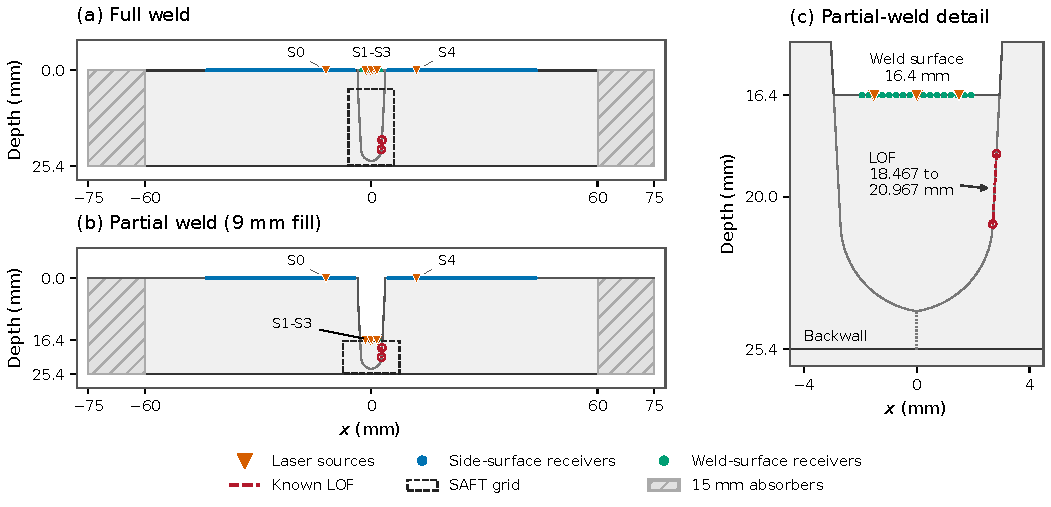
\includegraphics[width=\linewidth]{figures/saft_appendix/combined_explanatory/geometry.pdf}
\caption{Specimen geometry and acquisition. Orange triangles identify the two shoulder sources S0/S4 and three weld-surface sources S1--S3. Blue and green points denote side-surface and weld-surface receivers. The specimens include 15 mm absorbing strips at each lateral end. Separate dashed boxes show the actual full- and partial-weld reconstruction fields. The enlarged partial-weld detail shows the exposed floor, continuous J root and prescribed LOF. The grey internal outline is bonded except along the red flaw segment; it is not an open groove boundary below the fill.}
\label{saftapp:geometry}
\end{figure}

The five source coordinates are $x=-12,-1.5,0,1.5,12$ mm. S0 and S4 are shoulder sources at the original outer surface. S1--S3 lie on the exposed weld surface: $z=0$ in the full weld and $z=16.4$ mm in the partial weld. Both specimens have 157 receivers on each side surface at 0.25 mm pitch, extending to approximately $x=\pm43.5534$ mm. There are also 23 full-weld or 17 partial-weld receivers on the central weld surface, giving 337 and 331 receivers respectively. Every receiver measures vertical velocity $v_y$, which is normal motion on these horizontal receiving surfaces.

Five flawed and five pristine source simulations are available for each weld state: twenty production solves in total. Every recording contains 5001 samples over 50 $\mu$s at 10 ns output spacing. A pristine simulation has the same geometry and source but no separation. It provides an interpretation control and permits signed waveform subtraction; it is not an input to the LOF-only imaging recipe.

\subsection{Elastic propagation and numerical scope}
Production calculations use COMSOL Multiphysics 6.4, build 429, with the Elastic Waves, Time Explicit interface. Steel is homogeneous, isotropic and linearly elastic, under two-dimensional plane strain. The model uses $E=212.443$ GPa, $\nu=0.288978$ and $\rho=7859.975$ kg\,m$^{-3}$, giving longitudinal and in-plane shear speeds of $c_L=5943.60$ and $c_S=3237.97$ m\,s$^{-1}$. The corresponding Rayleigh speed used for arrival screening is $c_R=2997.33$ m\,s$^{-1}$. Longitudinal motion is primarily parallel to propagation; shear motion is transverse. Both can contribute to measured normal surface velocity after interaction with a free surface.

The elastic field satisfies
\begin{equation}
 \rho\,\ddot{\mathbf u}=\nabla\!\cdot\boldsymbol\sigma,
 \qquad \boldsymbol\sigma=\lambda\,\mathrm{tr}(\boldsymbol\varepsilon)\mathbf I
                 +2\mu\boldsymbol\varepsilon,
 \qquad \boldsymbol\varepsilon=\tfrac12(\nabla\mathbf u+\nabla\mathbf u^{\top}).
\end{equation}
Here $\mathbf u$ is displacement and $\lambda,\mu$ are the Lam\'e constants. Exposed surfaces and the LOF are traction-free except where the equivalent source acts. Bonded internal boundaries transmit displacement and traction. Weld and surrounding steel have identical properties, so the bonded fusion outline is not itself an impedance reflector. Absorbing strips at the lateral ends reduce artificial returns from the truncated specimen.

The production discretization uses quartic velocity and strain fields, a discontinuous Galerkin formulation and explicit fourth-order Runge--Kutta integration. Maximum element sizes are approximately 0.32380 mm in the weld and 0.48570 mm in the surrounding material, chosen using a 5 MHz design frequency. That choice does not establish a sharp accuracy cutoff at 5 MHz; receiver-level mesh and time-step convergence would be needed to establish a validated bandwidth. Likewise, the 50 MHz Nyquist frequency of the stored histories describes sampling, not the accuracy of the elastic solution. The 10 ns output interval must not be confused with the internal solver step.

\subsection{Calibrating the laser-equivalent source}
\label{saftapp:calibration}
The production source is an equivalent tangential traction representing thermoelastic expansion from an absorbed laser line. It is not an arbitrary point force adjusted to brighten the LOF. The calibration uses an independent 8 mm by 4 mm flat specimen, implemented with a 4 mm symmetric half-width. COMSOL Heat Transfer in Solids supplies the temperature field to Solid Mechanics through thermal expansion; a second mechanical field on the same mesh receives the candidate equivalent traction.

For a Gaussian laser profile, define $\xi=(x-x_s)/w$ with $w=0.5$ mm the $1/e^2$ radius. The absorbed heat flux is
\begin{equation}
 q(x,t)=\frac{F_0}{\sqrt{2\pi}\sigma_t}
 \exp(-2\xi^2)\exp\!\left[-\frac{(t-t_0)^2}{2\sigma_t^2}\right],
 \qquad \sigma_t=\frac{6.5\ \mathrm{ns}}{2\sqrt{2\ln2}}.
\end{equation}
The pulse centre is $t_0=30$ ns, or 0.030 $\mu$s. It is prescribed so the short Gaussian pulse lies inside the simulated time window; it is not a fitted imaging delay. $F_0$ is peak absorbed fluence. A 100 J\,m$^{-2}$ absorbed input is used for the production source, without assuming an optical absorptivity or equating it to incident laser energy.

The equivalent surface load is a tangential dipole,
\begin{equation}
 t_x(x,t)=4A\xi e^{-2\xi^2}H(t),\qquad t_y=0,
 \qquad H(t)=\tfrac12\left[1+\operatorname{erf}\!\left(\frac{t-t_0}{\sqrt2\sigma_t}\right)\right],
\end{equation}
with
\begin{equation}
 A=\gamma\frac{E\alpha F_0}{(1-\nu)\rho c_p w}.
\end{equation}
The opposing tangential lobes represent the lateral effect of a thin heated region. The finite source width is important to its angular and frequency response~\cite{tu}. Thermal inputs are $T_0=293.15$ K, conductivity 52 W\,m$^{-1}$\,K$^{-1}$, $c_p=480$ J\,kg$^{-1}$\,K$^{-1}$ and expansion coefficient $\alpha=11\times10^{-6}$ K$^{-1}$, following the material benchmark used for the calibration~\cite{dolz-2024}.

Only the scalar gain $\gamma$ is fitted. Signed horizontal and vertical velocity histories at five points on a 2 mm radius arc, from $15^\circ$ to $75^\circ$, are compared over 0.12--0.82 $\mu$s. Both fields receive the same forward--backward fourth-order 5 MHz Butterworth filter for this calibration comparison. If $\mathbf d$ is the unit-gain dipole history and $\mathbf v$ the thermoelastic history, the least-squares result is
\begin{equation}
 \gamma=\frac{\mathbf d^{\top}\mathbf v}{\mathbf d^{\top}\mathbf d}=1.084434.
\end{equation}
Figure~\ref{saftapp:source} shows the calibration comparison. The relative waveform error is 0.931\%; held-out axial and surface checks give approximately 1.09\% and 1.27\%. No angle-dependent gain, time shift or flaw response is fitted. The 10 and 100 J\,m$^{-2}$ calibrations give the same gain. At the production fluence, $A=188.939$ kPa and the maximum dipole traction is 229.195 kPa.

\begin{figure}[!htbp]\centering
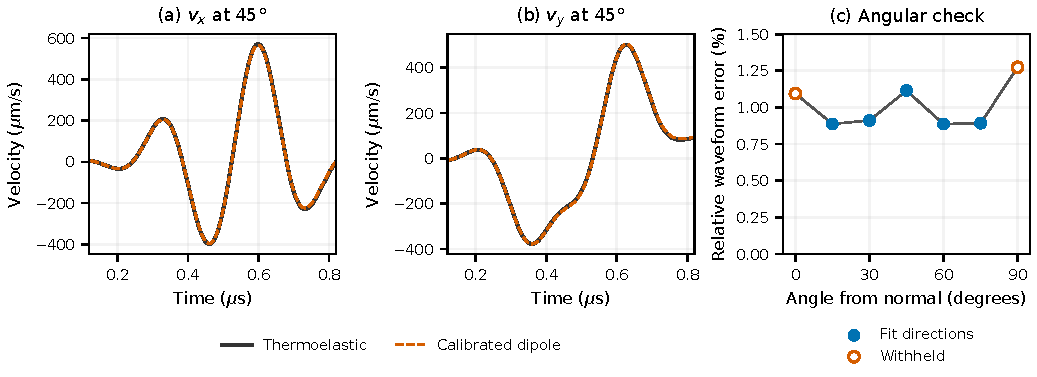
\includegraphics[width=.96\linewidth]{figures/saft_appendix/combined_explanatory/source_calibration.pdf}
\caption{Independent source calibration. The equivalent traction is compared with the thermoelastic calculation through signed outgoing velocity histories and angular response, rather than through a reconstructed flaw image. A single gain scales the dipole. Agreement supports this equivalent source over the tested calibration band and observation region; it does not establish production-mesh convergence or optical receiver sensitivity.}
\label{saftapp:source}
\end{figure}

\subsection{Source-calibration discretization and independent checks}
The small thermoelastic benchmark resolves the thin heated region with nine
surface-normal layers of thickness 0.05, 0.10, 0.20, 0.40, 0.80, 1.60, 3.20,
6.40 and 12.80 $\mu$m, totalling 25.55 $\mu$m. Eighty elements span the 4 mm
half-width and the bulk maximum size is 0.08 mm. Implicit generalized-$\alpha$
integration uses a maximum step of 0.5 ns during the first 60 ns and 2 ns
thereafter. The exported comparison contains 451 samples from 0 to
0.9 $\mu$s at 2 ns spacing. These are calibration-model settings, distinct
from the explicit production-weld calculation and its 10 ns output clock.

At 100 J\,m$^{-2}$ absorbed peak fluence, the integrated deposited energy per
out-of-plane length is 0.0626657 J/m, agreeing with the prescribed Gaussian
input within 0.000639\%. The temperature rise is 78.34 K; at 10 J\,m$^{-2}$
it is 7.83 K. The thermal field agrees with the independent one-dimensional
heat-flow check to 0.0693\% relative $L_2$, and differentiating displacement
agrees with exported velocity to 0.0481\%. These checks address input energy,
thermal consistency and mechanical output consistency. The sub-percent
outgoing waveform fit then addresses the particular equivalent-source
approximation. They are separate from production-mesh convergence and from
any reconstructed-image metric.


\section{Recorded wave fields in the two welds}

\subsection{What the full-weld recordings contain}
\begin{figure}[!htbp]\centering
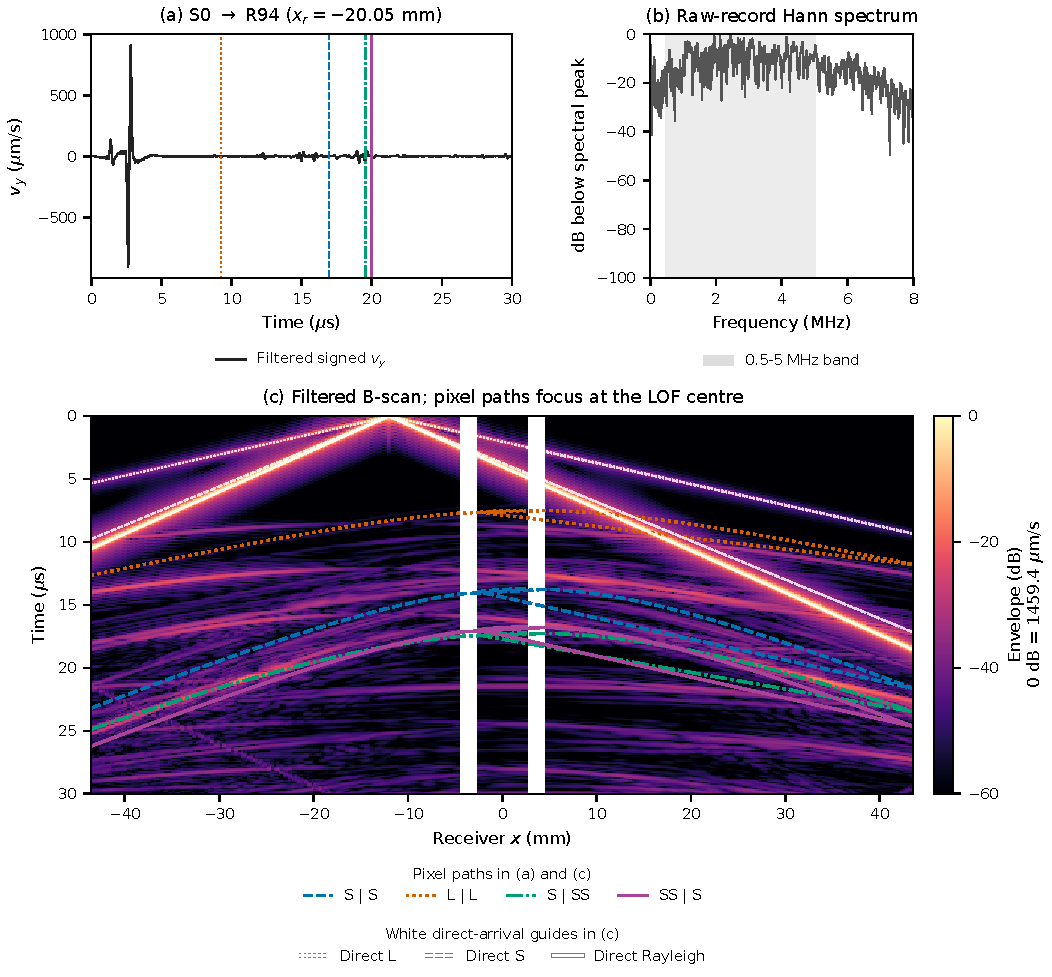
\includegraphics[width=.94\linewidth]{figures/saft_appendix/comsol/full_recordings.pdf}
\caption{Recording-level context with the common 0.5--5 MHz filter. The S0/R94 A-scan is one receiver history; the S0 B-scan stacks histories by receiver position. Coloured travel-time guides assume scattering at the known LOF centre: $S\mid S$ blue dashed, $L\mid L$ orange dotted, $S\mid SS$ green dash-dot and $SS\mid S$ purple solid. White direct-arrival guides are L dotted, S dashed and Rayleigh solid. These guides label timing hypotheses, not measured mode identities. The raw Hann-window spectrum has its own peak normalization. Filter-edge samples appear in this explanatory plot but are excluded where reconstruction lacks complete input support.}
\label{saftapp:archive:full:recordings}
\end{figure}

Read Figure~\ref{saftapp:archive:full:recordings} from the recording to the geometry. The A-scan shows that large motion occurs even before an identifiable flaw-scattering interpretation is available. The B-scan shows that these arrivals have systematic moveout across receivers. The spectrum shows available frequency content, but does not identify which frequencies belong to the flaw. The travel-time guides add a predicted interpretation to the data; a bright band meeting a guide is suggestive, not proof.

A pristine specimen still launches and reflects waves. Much of the prominent source-associated field is therefore expected in both simulations. Its persistence in an LOF-only image is a focusing ambiguity, not evidence that the imposed source has somehow moved into the weld. Increasing the minimum image depth only hides shallow pixels; it does not remove a source packet from the recorded histories. The following reconstruction instead checks path geometry and arrival time before combining samples.

\subsection{Why the source-associated field is particularly important here}
The LOF tips lie only 2.067--4.567 mm below the exposed weld surface. At the shear speed of 3.238 mm/$\mu$s, a short local round trip can occupy only a few microseconds. The generated field, its surface motion and early structural returns can therefore overlap the time range that would contain a direct flaw echo. A large recorded amplitude in that interval is not uniquely attributable to the LOF.

\begin{figure}[!htbp]\centering
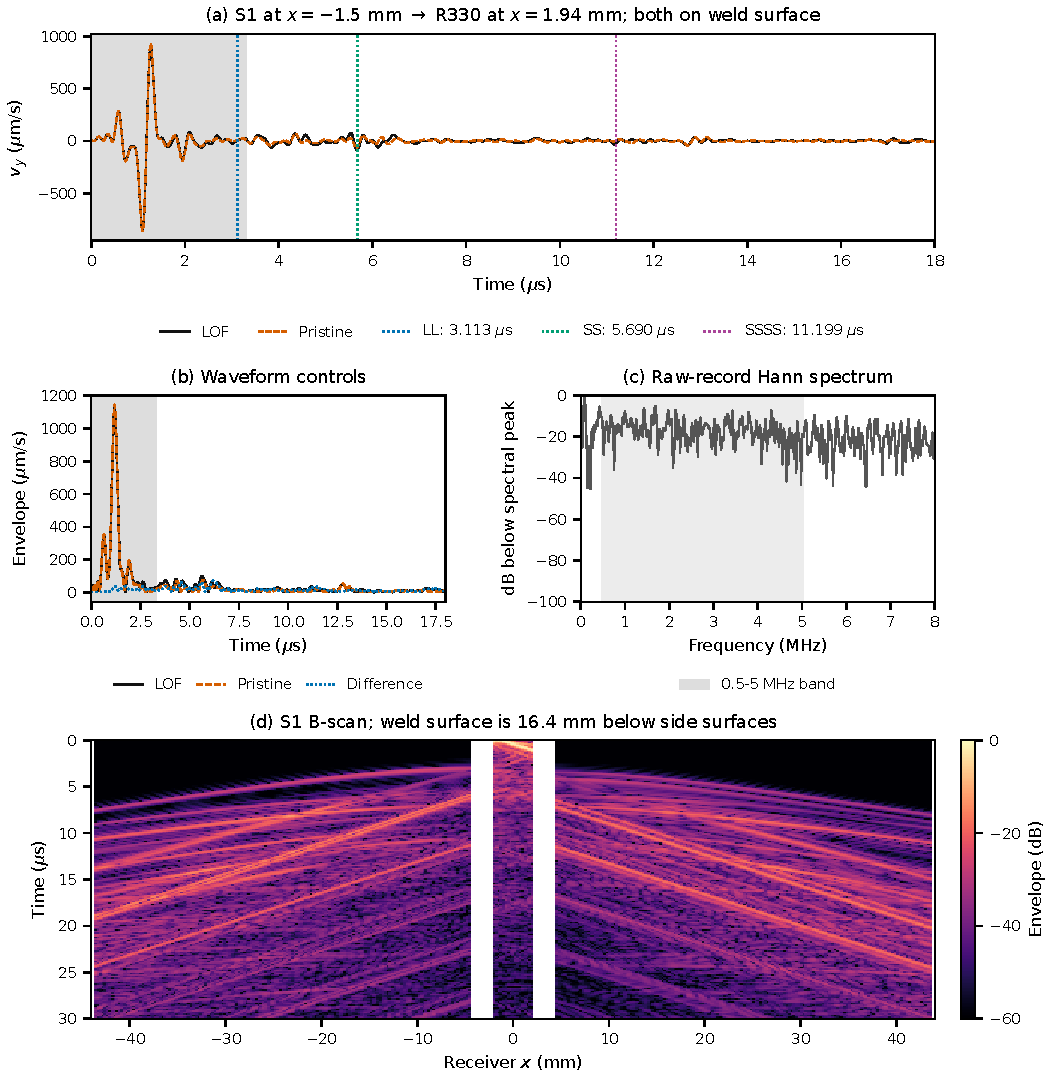
\includegraphics[width=\linewidth]{figures/saft_appendix/comsol/partial_recordings.pdf}
\caption{Partial-weld recording context for weld-surface source S1 and receiver R330. Traces and envelopes use the common 0.5--5 MHz processing; the spectrum uses the raw recording with a Hann window. LL at 3.113 $\mu$s, SS at 5.690 $\mu$s and SSSS at 11.199 $\mu$s denote specimen-only returns with no trial scattering point. Grey early-time shading indicates incomplete filter support. The B-scan has a separate reference of 1449.18 $\mu$m/s. The strong early field is present in both flawed and pristine recordings.}
\label{saftapp:archive:partial:recordings}
\end{figure}

Figure~\ref{saftapp:archive:partial:recordings} should be read as evidence of superposition. Flawed and pristine histories both contain the early packet. Later bands can include floor/backwall reverberation as well as flaw scattering. The white or coloured time guides are predictions superimposed on this field; they are not a decomposition of the measured signal into modes.


\section{Detailed reconstruction method}
\label{saftapp:method}
\subsection{A pixel represents a scattering hypothesis}
SAFT asks whether different receiver histories contain motion at the times expected if ultrasound scattered at a trial pixel $\mathbf p$. For each source $s$, receiver $r$ and chosen path $P$, it predicts
\begin{equation}
 T_{sr,P}(\mathbf p)=t_0+\sum_{j\in P}\frac{\ell_j(\mathbf p)}{c_{m_j}},
\label{saftapp:delay}
\end{equation}
where each leg has length $\ell_j$ and mode $m_j\in\{L,S\}$. The path notation places a vertical bar at the trial scattering point. Thus $S\mid S$ is direct shear illumination and direct shear reception; $S\mid SS$ adds one backwall reflection on the receiving route; $SS\mid S$ adds it on the incident route. $L\mid L$ is the direct longitudinal view. The notation describes the focusing hypothesis, not a measured separation of modes in the recordings.

Every segment must remain in steel and every reflection must lie on an actual boundary. In the partial weld, a ray cannot cross the open groove merely because its straight-line length is convenient. Valid routes may use the original surface, the exposed fill floor or the backwall where those surfaces exist. For a specified family, the implementation uses the earliest geometrically valid branch. The source and receiver sets are evaluated at every image pixel; a single inspection point does not define the whole image aperture.

\begin{figure}[!htbp]\centering
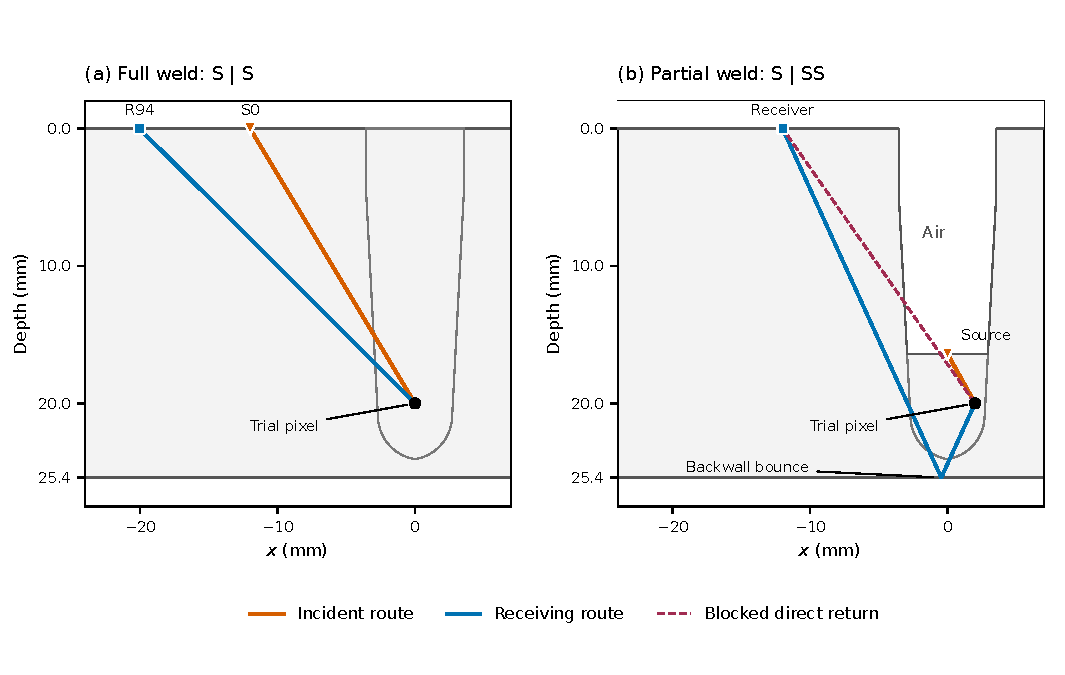
\includegraphics[width=.98\linewidth]{figures/saft_appendix/combined_explanatory/path_examples.pdf}
\caption{Illustrative focusing routes, with equal horizontal and depth scales. (a) A full-weld $S\mid S$ route from a shoulder source to a trial pixel and side receiver. (b) In the partial weld, direct illumination from the weld surface and a backwall-reflected return can remain inside steel even when a direct return crosses the open groove. These are worked geometric examples, not identified wave packets or additional measurement positions. The pale internal J outline is bonded; the white groove is air.}
\label{saftapp:paths}
\end{figure}

For example, a full-weld source at $(-12,0)$ mm, receiver at $(-20.0534,0)$ mm and pixel at $(0,20)$ mm give a direct-S delay of about 15.98 $\mu$s; the same lengths give about 8.72 $\mu$s for direct L. In the partial-weld example, a source at $(0,16.4)$ mm illuminates $(2,20)$ mm and returns through a backwall bounce to an illustrative receiver at $(-12,0)$ mm. The incident length is 4.118 mm and the reflected receiving length is 33.833 mm, giving $T=11.751$ $\mu$s. The direct return would cross the fill depth at $x=-0.52$ mm, inside the open groove, and is invalid. The reflected return crosses that depth at about $x=-7.91$ mm, in steel. This is why a reflected view can be necessary, rather than merely an optional extra image.

\subsection{Admitting useful launch and receive angles}
A laser dipole does not launch all modes equally in all directions. A normal-motion receiver also does not observe every incoming mode equally. Free-surface reflection and conversion contribute to its response, so normal sensitivity cannot be estimated from the incident displacement component alone. The baseline study uses the angular magnitudes in Figure~\ref{saftapp:coupling} to admit plausible channels.

\begin{figure}[!htbp]\centering
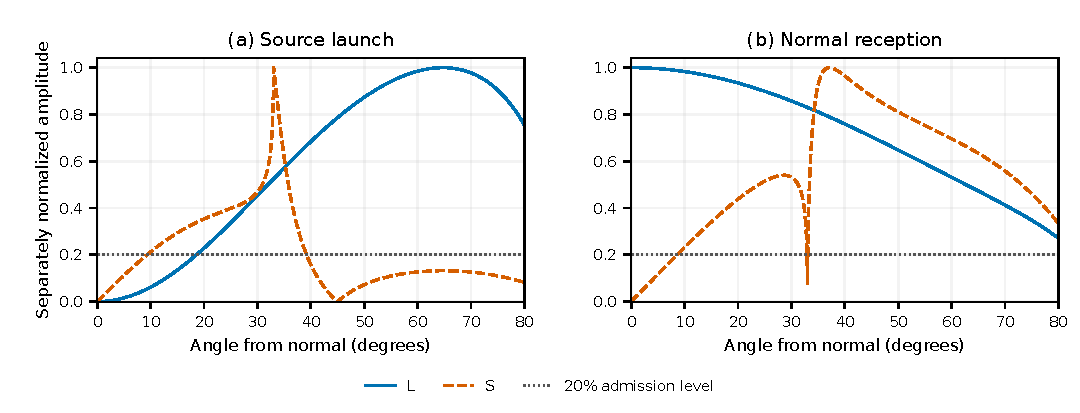
\includegraphics[width=.92\linewidth]{figures/saft_appendix/combined_explanatory/coupling.pdf}
\caption{Angular launch and normal-reception magnitudes used for channel admission. L and S are normalized separately, so the curves do not compare absolute longitudinal and shear energy. The 20\% level is a selection threshold: a channel must satisfy both its source and receiver tests. The baseline averages admitted receivers equally; the updated partial-weld recipe also uses their complex response. These curves explain why a large spatial aperture can still contain unsuitable mode/path combinations.}
\label{saftapp:coupling}
\end{figure}

In the baseline, for a channel to qualify, both normalized launch and receive magnitudes must reach 20\%, and receive angle must not exceed $80^\circ$ from the normal. A reflected route must also pass a 5\% wall-response-product gate. These are admission tests, not amplitude weights or phase corrections. A 1.5 mm source--receiver separation exclusion keeps receivers outside the approximately 1.425 mm source-footprint half-width. The wall gate is inactive for the principal images but affects some longer partial-weld paths. Removing the separation exclusion changes the principal images measurably. Both controls are therefore retained as declared physical rules; detailed ablations are in this appendix.

\subsection{Frequency filtering and pulse-aware screening}
\label{saftapp:time}
The recorded field includes direct bulk waves, surface motion, reflected packets and flaw scattering. A strong direct packet can be sampled at a delay assigned to a deep trial pixel and create an apparent indication. Its coherence across receivers means that ordinary averaging, or even coherence weighting, may preserve it. The contamination is therefore a mismatch between the packet's actual route and the route assumed in focusing. Cropping shallow pixels does not remove that packet from the histories.

The common comparison uses a 657-tap analytic finite impulse response (FIR) filter over 0.5--5 MHz, with Kaiser parameter 5.10226. It supplies a complex signal with amplitude and phase for delay-and-sum processing. At 10 ns spacing its half-support is 3.28 $\mu$s. Reconstruction requires complete filtering and interpolation support, giving a usable delay interval of approximately 3.28--46.71 $\mu$s. The filter suppresses components outside a declared analysis band; it is not justified by the stored sampling limit, nor does it prove the mesh resolves all retained frequencies accurately.

Direct L, S and Rayleigh arrivals are then screened per source--receiver pair. A geometry-valid prediction locates an envelope peak within $\pm0.25$ $\mu$s. The packet window extends until the envelope is below $-30$ dB relative to that peak for at least 0.15 $\mu$s, with a further 0.1 $\mu$s margin. An imaging sample falling within the excluded window is not admitted. This avoids a single fixed mute duration for packets with different widths. The finite search reach is tied to the source/filter pulse. Rayleigh screening requires a common unobstructed flat surface; it does not assume a surface wave crosses the empty groove.

The same rule acts differently in the two geometries. All 1685 full-weld source--receiver pairs have direct bulk paths. Only 365 of 1655 partial-weld pairs have direct paths: shoulder-to-side pairs on their own side and weld-surface pairs on the floor. Applying flat-surface direct-arrival predictions to the remaining pairs would exclude samples using physically invalid paths. The baseline images use this direct-arrival screening with fixed mutes and reflected-arrival screening off. The updated partial-weld recipe adds the narrow fixed mute defined below.

The screening windows for an LOF-only image are obtained from its own recording. A pristine image uses its own windows; the waveform-difference control uses the LOF-derived windows. The procedure therefore requires no reference recording to suppress the direct field. It can still reject real flaw information when arrivals overlap, especially for a source close to the partial-weld flaw. This cost appears as lost support and must be reported alongside contrast.

Fourteen filter alternatives are documented in this appendix, including unfiltered and unrestricted-band controls. For the selected full-weld direct-S image, a shorter 257-tap 0--5 MHz low-pass is used, while retaining the same 3.28 $\mu$s admission guard. The historical partial-weld results retain the common 657-tap bandpass; the revised weighted recipe uses 1--5 MHz with the same tap count and guard. These are explicitly different selected recipes; the common four-path full-weld comparison retains identical filtering. The source-calibration Butterworth filter is a separate operation and is not the reconstruction FIR.

\subsection{Baseline receiver averages, coherence and source coverage}
Let $a_{sr}(\mathbf p)$ be the complex filtered history interpolated at Equation~\ref{saftapp:delay}, after the channel and timing tests. For $N_s$ admitted receivers, the equal mean and receiver coherence factor are
\begin{equation}
 M_s(\mathbf p)=\frac{1}{N_s}\sum_r a_{sr}(\mathbf p),\qquad
 \mathrm{CF}_s(\mathbf p)=\frac{|\sum_r a_{sr}(\mathbf p)|^2}
 {N_s\sum_r|a_{sr}(\mathbf p)|^2}.
\label{saftapp:cf}
\end{equation}
The coherence factor is zero for zero signal energy and otherwise lies between zero and one. Aligned phases reinforce in the numerator; inconsistent phases reduce it. The factor has exponent one here. It encourages phase consistency under the selected delay law, but a coherent structural echo can also pass that test. This equation describes the equal-mean baseline. Response weighting for the updated partial-weld result is defined below.

Each source must retain at least eight receivers and at least 25\% of its aperture eligible before the time-support and pulse tests. With equal receiver weights, effective receiver count equals actual count. The nominal image requires at least two qualifying sources at a pixel. If $\mathcal S(\mathbf p)$ is that set, source results combine as
\begin{equation}
 I(\mathbf p)=\left[\frac{1}{|\mathcal S|}\sum_{s\in\mathcal S}
                 |\mathrm{CF}_s M_s|^2\right]^{1/2}.
\label{saftapp:source_rms}
\end{equation}
This root-mean-square combination avoids cancellation between separately illuminated source views. The output retains velocity units but is a processed focusing score, not acoustic intensity or flaw size. A pixel failing the required source count is unsupported; it is not assigned a physical zero.

Allowing one qualifying source changes which pixels can be displayed. It does not mean acquiring only one laser shot for the whole image: all selected source shots remain available wherever they qualify, and Equation~\ref{saftapp:source_rms} still uses them. This distinction is essential to the partial-weld coverage comparison below.

\subsection{Response weighting and a narrow reflected-arrival mute}
The revised partial-weld comparison uses the existing response-weighted option. Let $b_{sr}$ be the complex product of the predicted wall and normal-reception responses and let $w_{sr}=|b_{sr}|$. After interpolation and any mute, the sample is $a_{sr}$. The implemented sums are
\begin{equation}
 Q_s=\sum_r a_{sr}b_{sr}^{*},\quad W_s=\sum_r w_{sr},\quad
 P_s=\sum_r w_{sr}|a_{sr}|^2,\qquad
 M_s=Q_s/W_s,\quad \mathrm{CF}_s=\frac{|Q_s|^2}{W_sP_s}.
\label{saftapp:weighted}
\end{equation}
Thus the response supplies a phase correction as well as an amplitude weight. It is not inverse-amplitude compensation. Source directivity remains an admission test; an unknown flaw-scattering coefficient is not fitted. The effective receiver count is $N_{\mathrm{eff}}=W_s^2/\sum_r w_{sr}^2$. Setting every $b_{sr}=1$ recovers the equal-mean baseline. The revised images retain $\mathrm{CF}^1$, RMS source combination, eight actual and eight effective receivers, the 25\% retention rule and a two-source minimum unless stated otherwise.

The revised partial-weld working choice uses a 657-tap 1--5 MHz band, a 15\% angular gate and an additional smooth mute about the geometry-valid, specimen-only backwall $SS$ arrival. This arrival travels from source to backwall to receiver without the trial scattering point. For its predicted time $t_{SS}$, set $d=|T-t_{SS}|/h$ and
\begin{equation}
 g(T)=\tfrac12\{1-\cos[\pi\,\operatorname{clip}((d-0.75)/0.25,0,1)]\},
 \qquad a_{sr}=g(T)\,a_{sr}^{\rm filtered},\quad h=0.30\ \mu\mathrm{s}.
\label{saftapp:mute}
\end{equation}
Samples within $\pm0.225$ $\mu$s are rejected; the taper reaches full weight at $\pm0.30$ $\mu$s. The original direct L/S/R pulse screens and complete FIR support remain active. This short, predicted-arrival mute is a separate hypothesis from rejecting the entire measured reflected packet. It removes only its central timing region and cannot establish that all reflected contamination has been removed. Its width is selected retrospectively from the sensitivity study, not measured as a universal pulse duration.

\subsection{Image fields, controls and numerical comparisons}
\label{saftapp:metrics}
The full-weld grid spans $x=\pm6$ mm and requested depths 5--25.25 mm; the partial-weld grid spans $x=\pm7.5$ mm and 16.65--25.25 mm. Baseline principal images use 0.1 mm pixels; the revised partial-weld result is also checked at 0.025 mm and with a shifted grid. Sampling from the full-weld start depth places its last row at 25.2 mm. At 5 MHz the shear wavelength is approximately 0.648 mm, so the pixel grid samples the image finely but does not establish 0.1 mm physical resolution. Finer 0.05 mm grids and wider $x=\pm45$ mm fields check peak stability and competing indications.

The images show $20\log_{10}[I(\mathbf p)/I_0]$ over a declared display range: 45 dB for the principal path and source-threshold panels, and 40 dB for the partial-weld acquisition comparison. A shared reference is used within each comparison. Black denotes low displayed amplitude, grey denotes unsupported material, and white denotes air. Thin external LOF guides identify the prescribed location without covering the image. These marks are ground-truth annotations, including in pristine panels, not a reconstructed flaw outline.

Define a near-flaw region $\mathcal N$ within 0.5 mm of the finite prescribed segment and a background region $\mathcal B$ more than 1 mm from it. The intervening buffer is omitted. Over supported pixels,
\begin{equation}
 C_{\max}=20\log_{10}\frac{\max_{\mathcal N}I}{\max_{\mathcal B}I},\qquad
 C_{99}=20\log_{10}\frac{\max_{\mathcal N}I}{Q_{99,\mathcal B}(I)}.
\end{equation}
Positive $C_{\max}$ means the strongest near-flaw response exceeds every assessed background pixel. Near-flaw support is the fraction of $\mathcal N$ with a valid image value. It is not the fraction of flaw length detected. Changing an aperture changes both the signal and the assessed region; comparisons therefore report support and, where needed, restrict both images to a common mask.

The LOF-only image is the principal result. Pristine controls test whether the intact structure produces a similar indication. Difference controls subtract signed LOF and pristine waveforms before filtering and focusing; they do not subtract displayed image amplitudes. Since interference and coherence change, a difference image can have a larger peak than the LOF-only image. These controls support attribution to the flaw but do not establish a detection threshold from one simulated defect.

\subsection{Implementation verification and reproduction scope}
The archived verification checks dataset fingerprints, receiver coordinates
and the time clock before reconstruction. An independent bandpass calculation
for four paths, five points and three signal cases in each geometry agrees
with the native C++ engine within $5.4\times10^{-19}$ m\,s$^{-1}$.
A sinusoidal input checks gain and phase. The archived laser regression run
contains 242 passing tests. Image checks independently recompute coordinate
bounds, amplitude/support consistency, contrasts and peak locations. These
are implementation checks, not a substitute for experimental validation.

The primary reconstruction archive contains 104 full-weld and 280
partial-weld configurations, each with LOF, pristine and waveform-difference
images. The joint-acquisition supplement adds 25 scientific partial-weld
configurations and one numerical replay control. Thus the primary and joint
studies contain 104 full-weld and 305 partial-weld scientific configurations;
gate and additional-geometry audits are separate. These are reconstructions
of the production recordings, not additional COMSOL solves. The repository
retains protocols, model/dataset metadata, numerical arrays, settings and
verification scripts. The portable LaTeX edition contains the complete
explanation and figures; it does not embed the raw simulation recordings.


\section{Filter definitions and baseline variants}
\subsection{Filter definitions and controlled processing variants}\label{saftapp:archive:shared:filter_details}
The purpose of this comparison is to distinguish three effects: which frequencies are retained, how long the temporal averaging kernel is, and which arrival times are admitted. These can change independently. Holding the admission guard fixed while shortening a filter tests its waveform effect without automatically gaining earlier samples.

The survey holds geometry, source/receiver lists, physical gates, coherence, source qualification and combination fixed. Four full-weld and eighteen partial-weld paths are processed with fourteen variants and three signal cases. This gives 168 full-weld and 756 partial-weld survey images. Finer-grid, wider-field, coupling and acquisition checks bring this primary archive to 384 configurations and 1152 signal-case images. The separately documented joint-acquisition supplement contributes 25 scientific configurations and one replay control. These counts refer to reconstructions of the existing production recordings, not new finite-element solutions.

For reproducibility, the filter coefficients are specified below. A finite sequence of coefficients weights neighbouring samples; the complex exponential shifts the selected band, and the Kaiser window limits sidelobes. For the FIR variants the analytic kernel is
\begin{equation}
 h_n=\frac{2b_n}{\sum_k b_k}\exp(2\pi if_cn\Delta t),\quad
 b_n=2B\Delta t\,\operatorname{sinc}(Bn\Delta t)K_\beta(n),
\end{equation}
where $B=f_H-f_L$, $f_c=(f_H+f_L)/2$, $\operatorname{sinc}(u)=\sin(\pi u)/(\pi u)$ and $K_\beta$ is a Kaiser window with $\beta=5.10226$. The ordinary positive-frequency gain is approximately two. Nominal edges fall in finite transition bands, rather than defining brick-wall cutoffs. At low frequencies, including DC, the response differs from an ideal analytic transform; Figure~\ref{saftapp:archive:shared:filters} displays that response explicitly.

\begin{figure}[htbp]\centering
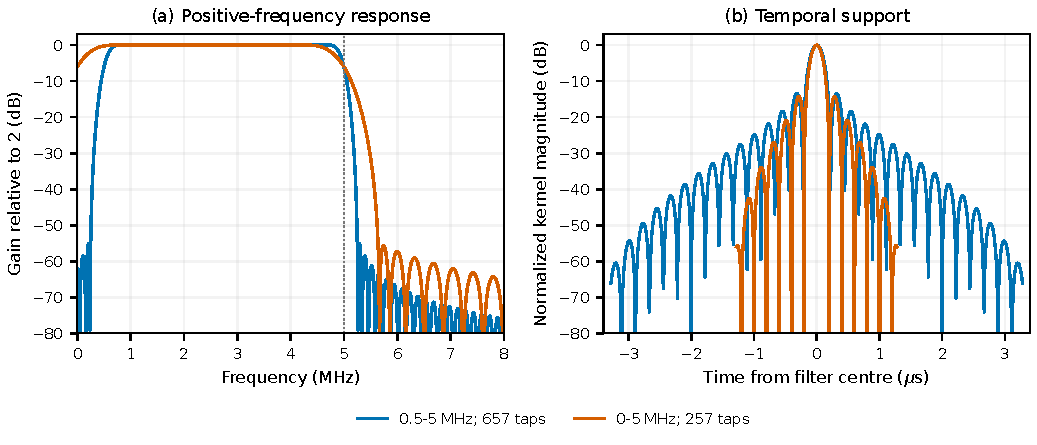
\includegraphics[width=\linewidth]{figures/saft_appendix/comsol/filter_response.pdf}
\caption{Frequency response and temporal kernel magnitude for the two selected filters. Both selected images retain a 3.28 $\mu$s admission guard even though the 257-tap kernel itself has 1.28 $\mu$s half-support. This separates shorter temporal averaging from recovery of earlier samples.}
\label{saftapp:archive:shared:filters}
\end{figure}

\begin{table}[htbp]\centering\small
\caption{All processing variants. The initial-rest extension admits known zero prehistory but retains rejection of the unknown post-record tail. A stated guard is independent of kernel duration.}
\label{saftapp:archive:shared:variants}
\begin{tabularx}{\linewidth}{@{}Xrr@{}}\toprule
Processing & Taps & Guard ($\mu$s)\\\midrule
0.5--5, 1--5, 0.5--3, or 0--5 MHz analytic FIR & 657 & 3.28\\
0.5--5 MHz analytic FIR, matched long guard & 257 & 3.28\\
0.5--5 MHz analytic FIR, native guard & 257 & 1.28\\
0--5 MHz analytic FIR, matched long guard & 257 & 3.28\\
0--5 MHz analytic FIR, native guard & 257 & 1.28\\
0--5 MHz analytic FIR, shorter kernel & 129 & 0.64\\
Original bandpass with known initial rest & 657 & 3.28\\
Short low-pass with known initial rest & 257 & 1.28\\
5 MHz forward--backward Butterworth, then analytic transform & -- & 3.28\\
Unrestricted-band analytic transform & -- & 3.28\\
Signed unfiltered samples & -- & 0\\\bottomrule
\end{tabularx}
\end{table}

The signed unfiltered case changes phase representation as well as bandwidth, so it is not an envelope-equivalent replacement. The unrestricted analytic case retains broad spectral content without claiming that the production mesh resolves all of it. Zero initial velocity is verified in every record before initial-rest continuation is used. For the noncompact analytic/Butterworth controls, 4096 zero samples precede the 5001-sample recording in a 32768-point transform. Doubling the transform length to 65536 changes usable-window waveforms by at most 0.0171\% relative $L_2$ across sources and signal cases. This checks sensitivity to the finite transform extension, not ideal finite-time analytic support.

The shorter selected full-weld filter leaves approximately 0.040--0.044\% of total processed-record energy above 5 MHz. This is a descriptive global energy fraction; it neither proves mesh accuracy nor bounds the error of a focused pixel. The survey is exploratory on a known simulated flaw. Confirmation checks test the stability of its interpretation, rather than converting the selected result into a universally optimal filter.


\section{Full weld: selected paths and signal controls}
\label{saftapp:full}
\label{saftapp:archive:full:principal}
\subsection{Four paths with the same processing rules}
The common comparison keeps the 657-tap 0.5--5 MHz filter, timing guard, physical gates, screening, coverage thresholds and equal receiver averaging fixed. Only the focusing path changes. Its eligible aperture still changes, because each path uses different angles and delays. This is a common-rule comparison, not a requirement that every path average identical receiver IDs.

\begin{figure}[!htbp]\centering
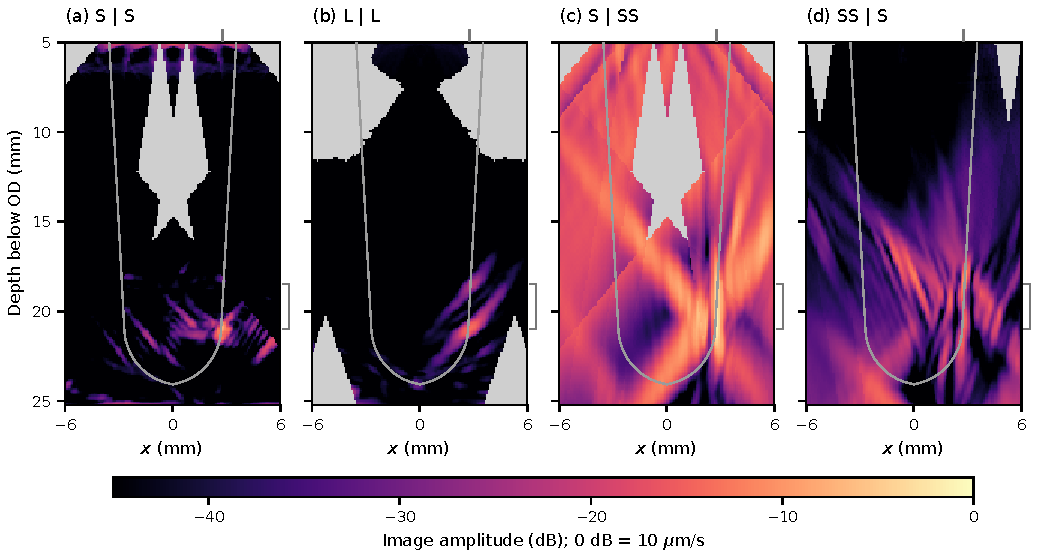
\includegraphics[width=\linewidth]{figures/saft_appendix/comsol/full_common_paths.pdf}
\caption{LOF-only full-weld images for the four tested paths with common processing and 0.1 mm pixels. All panels use 0 dB = 10 $\mu$m/s and a 45 dB range. Thin external marks identify the prescribed LOF; grey is unsupported. Direct views concentrate near the lower tip, while the reflected views are more extended. The result supports complementary localization, not a measurement of the full flaw outline.}
\label{saftapp:archive:full:common_overview}
\end{figure}

All four global maxima lie within 0.37 mm of the prescribed finite segment. Direct L gives $C_{\max}=8.85$ dB, direct S 6.47 dB, $S\mid SS$ 4.65 dB and $SS\mid S$ 4.37 dB. Each has 100\% near-flaw support. These results answer the first question: several path hypotheses yield a local indication with no pristine subtraction.

The location and shape carry different information. The direct views mainly emphasize the lower-tip vicinity. The broader reflected views sample a different angular relationship to the flaw, but their elongated bright regions can include the imaging point-spread function and structural interference. An image is a map of delay consistency; its bright extent cannot simply be read as physical flaw length.

The agreement of several views strengthens the interpretation, but they reuse the same simulations and are not independent detection trials. Their complete pristine and difference controls are retained in Section~\ref{saftapp:archive:full:complete}. A colour blend may help display complementary responses, but adding arbitrary path colours does not define a calibrated probability or improve the underlying acoustic information.

\subsection{Separate the filter question from the path question}
For direct S, the 657-tap common bandpass gives 6.47 dB contrast. A 257-tap filter with the same nominal 0.5--5 MHz edges gives 10.26 dB. A 257-tap 0--5 MHz low-pass gives 12.79 dB. All three retain the same 3.28 $\mu$s admission guard. The difference therefore involves the waveform being averaged, including temporal smearing and frequency content, rather than simply recovering previously excluded early samples.

The selected direct-S result uses the shorter low-pass. It should not be described as unfiltered, since high frequencies are still attenuated and the analytic phase representation is still used. Nor is it a universal best filter: direct L gives only 3.24 dB with the same shorter low-pass, compared with 8.85 dB under the common bandpass. A frequency choice is coupled to the scattering and timing hypothesis.

Fourteen alternatives, including unrestricted-band analytic and signed unfiltered reconstructions, are documented in the supporting comparison. Their role is to test the processing assumption, not to infer a validated frequency limit from the strongest known-flaw score. The selected filter is an exploratory choice on this modeled case.

\subsection{Selected direct-S image and its controls}
\begin{figure}[!htbp]\centering
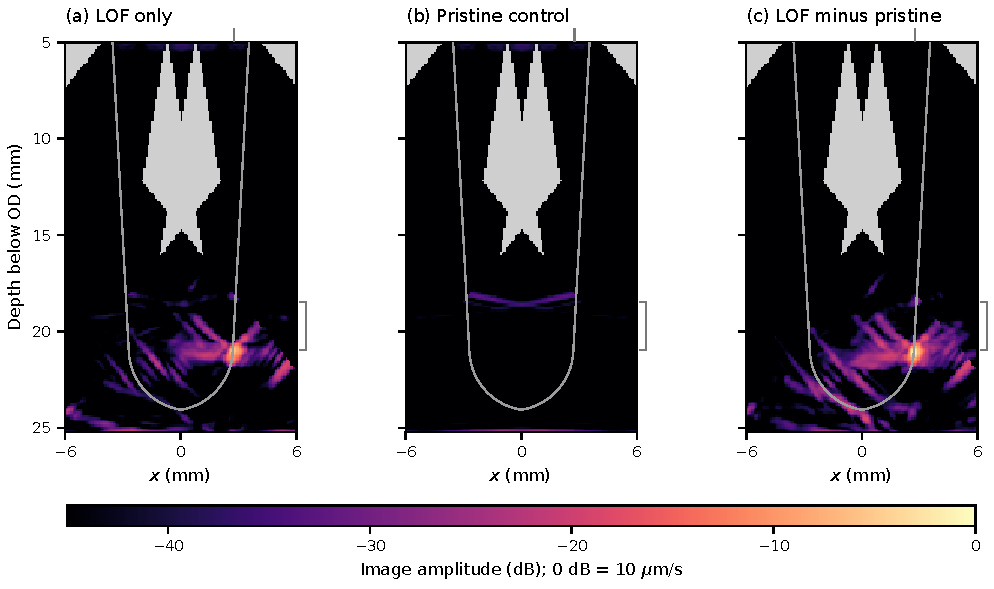
\includegraphics[width=.98\linewidth]{figures/saft_appendix/comsol/primary_full.pdf}
\caption{Selected $S\mid S$ reconstruction and its controls. Processing uses a 257-tap 0--5 MHz analytic FIR filter, the retained 3.28 $\mu$s admission guard and the common selection/coherence rules. All panels show the complete requested field at 0.1 mm spacing with 0 dB = 10 $\mu$m/s over 45 dB. The pristine panel has no physical flaw; its external marks identify the comparison coordinates.}
\label{saftapp:archive:full:selected}
\end{figure}

The LOF-only image peaks at 5.184 $\mu$m/s at $(2.7,21.0)$ mm, 0.0325 mm from the finite LOF segment. Its maximum-background contrast is 12.79 dB, its percentile contrast is 21.28 dB, and its near-flaw support is 100\%. The dominant indication lies at the lower-tip vicinity. The reported 0.0325 mm distance is a coordinate comparison, not an experimentally demonstrated localization accuracy finer than a pixel.

The pristine global maximum is 0.485 $\mu$m/s and occurs away from the flaw. The waveform-difference maximum is 8.791 $\mu$m/s at $(2.7,21.1)$ mm. Taken together, the strong flawed response, weak pristine response and local difference response support an association with introducing the separation. The difference peak is allowed to exceed the LOF-only peak: subtraction changes signed interference, source means and coherence. It is not equivalent to subtracting the two displayed amplitudes.

\subsection{Does the indication depend on a convenient crop or pixel size?}
At 0.05 mm spacing the selected direct-S contrast is 12.63 dB. In the wider $x=\pm45$ mm field at 0.25 mm spacing it is 10.62 dB and the global maximum remains near the flaw. This supports localization beyond one grid and one crop, while the changed support and background set explain why the numerical contrast need not remain identical.

\begin{figure}[!htbp]\centering
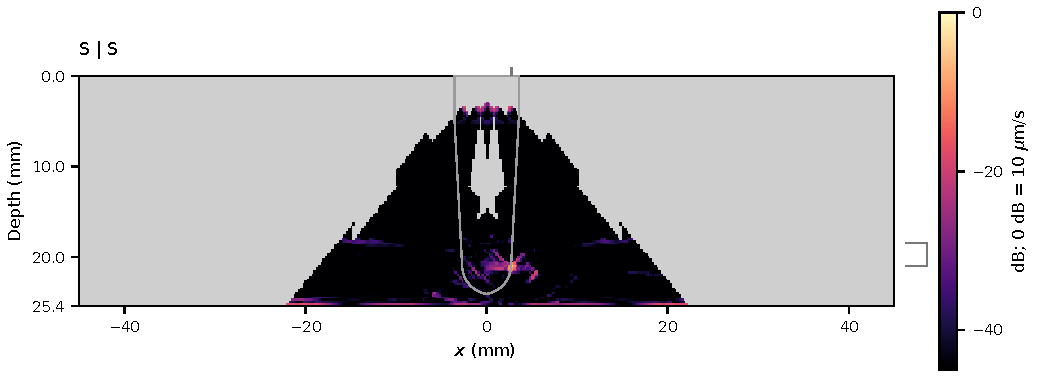
\includegraphics[width=\linewidth]{figures/saft_appendix/comsol/full_wide.pdf}
\caption{Selected direct-S image over the expanded field, at 0.25 mm spacing. The amplitude reference and 45 dB range match Figure~\ref{saftapp:archive:full:selected}. Grey areas are unassessed by the declared aperture rules. A wider image checks for competing supported maxima; it does not establish whole-specimen coverage.}
\label{saftapp:archive:full:wide}
\end{figure}

Changing the angular admission level to 15\% or 25\% gives 10.16 and 13.79 dB with complete near-flaw support. Recomputing the launch curve for the selected low-pass leaves that image unchanged. These checks support stability of the selected interpretation, but not every path behaves as well. The common-protocol $SS\mid S$ wider-field control has $C_{\max}=-17.80$ dB: a much stronger lateral artefact appears when the field is expanded. Local success must therefore be checked against a suitably broad background region.


\section{Full weld: source and receiver comparisons}
\label{saftapp:archive:full:acquisition_results}
Whole physical groups are removed while holding the selected processing fixed. This asks where useful acoustic information is available. It does not search for an arbitrary subset of individual channels that happens to maximize the known-flaw metric.

\begin{table}[!htbp]\centering\small
\caption{Source and receiver group reductions at 0.1 mm. Direct S uses the selected short low-pass; direct L uses the common bandpass. Near support measures available grid pixels, not detected flaw length.}
\begin{tabularx}{\linewidth}{@{}lXrr@{}}\toprule
Path & Acquisition & $C_{\max}$ (dB) & Near support (\%)\\\midrule
$S\mid S$ & All sources and receivers & 12.79 & 100.0 \\
$S\mid S$ & Shoulder sources only & 10.57 & 92.4 \\
$S\mid S$ & Weld-surface sources only & -20.66 & 9.8 \\
$S\mid S$ & Side-surface receivers only & 11.83 & 100.0 \\
$S\mid S$ & Weld-surface receivers only & -2.64 & 92.4 \\
$S\mid S$ & Shoulders and side-surface receivers & 9.61 & 92.4 \\
\addlinespace
$L\mid L$ & All sources and receivers & 8.85 & 100.0 \\
$L\mid L$ & Shoulder sources only & 8.85 & 100.0 \\
$L\mid L$ & Weld-surface sources only & -- & 0.0 \\
$L\mid L$ & Side-surface receivers only & 6.43 & 100.0 \\
$L\mid L$ & Weld-surface receivers only & -11.77 & 100.0 \\
$L\mid L$ & Shoulders and side-surface receivers & 6.43 & 100.0 \\
\addlinespace

\bottomrule\end{tabularx}
\label{saftapp:archive:full:groups}
\end{table}

For direct S, using only the two shoulder sources with all receivers gives 10.57 dB and 92.4\% near support. Retaining all sources but receiving only on the side surfaces gives 11.83 dB and complete near support. Combining shoulder generation with side-surface reception gives 9.61 dB and 92.4\%. This is a useful reduced physical arrangement: generation directly over the weld and reception on its narrow central surface are not essential to a local indication for this flaw.

Weld-surface generation alone is much less effective for direct S, giving negative contrast and only 9.8\% near support. This agrees with the need for suitable oblique illumination and a sufficiently large qualified aperture. It does not prove that these sources radiate no waves toward the flaw; it means that the complete reconstruction and qualification rules do not retain a useful local image from that group alone.

Direct L is retained in the group comparison because changing mode also changes launch and receive sensitivity. One cannot choose a receiver distribution solely from spatial coverage and then assume it is optimal for every path. The relevant spread is a spread of useful ray angles and delays, evaluated per source and per path.

These group tests justify an acquisition direction, not the smallest receiver count. The side groups still contain densely spaced positions. A subsequent sparse design should preserve angular and timing diversity within each useful source/path aperture, compare results on common support, and be tested on withheld flaw cases and noise. The present result does not justify deleting the remaining channels from a validated instrument design.


\section{Full weld: complete numerical comparisons}

\label{saftapp:archive:full:complete}
This section retains the complete evidence behind the preceding argument. First, the four-path atlas and table compare LOF, pristine and difference cases under the common protocol at 0.1 mm spacing. The filter definitions and matrix then compare fourteen processing variants on the 0.2 mm survey grid. Finally, the explicit ray expressions and confirmation register document the finer grids, wider fields and physical aperture tests. Values from different grids or fields should not be interpreted as changes in processing alone.

\subsection{Wall-response gate and source--receiver exclusion}
\label{saftapp:archive:full:gate_audit}
The wall gate (5\%) and source--receiver exclusion (1.5 mm) are disabled separately and jointly, with all other controls fixed. The audit includes the common-band path surveys and all confirmations: 52 full-weld and 46 partial-weld configurations. Three perturbations per configuration and three signal cases give 294 reconstructions and 882 paired image comparisons. Repeating the principal nominal settings checks the archived arrays.

Image change is measured before display clipping, over the intersection $\Omega$ of supported pixels:
\begin{equation}
 \delta_I=100\frac{\lVert I_{\rm test}-I_{\rm nominal}\rVert_{2,\Omega}}
 {\lVert I_{\rm nominal}\rVert_{2,\Omega}}\ \%.
\end{equation}
Support changes are assessed separately. Table~\ref{saftapp:archive:full:gate_controls} gives the principal LOF-only view; its support mask is identical in all four cases.

\begin{table}[htbp]\centering\small
\caption{Independent and joint gate checks for the principal
full-weld $S\mid S${}
image at 0.1 mm spacing. Zero disables the corresponding gate. $\delta_I$ measures whole-image amplitude change on common support; it is not a change in detection probability.}
\label{saftapp:archive:full:gate_controls}
\begin{tabular}{@{}lrrr@{}}\toprule
Wall gate / exclusion & $C_{\max}$ (dB) & $\delta_I$ (\%) & Near support (\%)\\\midrule
5\% / 1.5 mm & 12.79 & 0.00 & 100.0 \\
0\% / 1.5 mm & 12.79 & 0.00 & 100.0 \\
5\% / 0 mm & 13.12 & 6.56 & 100.0 \\
0\% / 0 mm & 13.12 & 6.56 & 100.0 \\

\bottomrule\end{tabular}
\end{table}

Disabling the wall gate alone leaves all 52 full-weld configurations exactly unchanged in all three signal cases. Direct paths have no intermediate wall reflection; the tested reflected paths also give identical images. The 5\% threshold is inactive here but retained in the shared protocol because multiple-reflection partial-weld routes are sensitive to it.

Disabling separation changes the principal image by 6.56\% and raises $C_{\max}$ from 12.79 to 13.12 dB without changing support. Disabling both controls gives the same image. This modest contrast increase for one known flaw does not establish that sampling within the source footprint is preferable.

The 1.5 mm exclusion avoids the 1.425 mm effective source footprint, where directly applied loading complicates interpretation as a remotely received wave. It does not guarantee background removal. The exclusion distance and 5\% wall threshold are declared engineering safeguards; neither has been established as a universal optimum.

\subsection{Complete common-protocol path and control comparison}
\begin{figure}[htbp]\centering
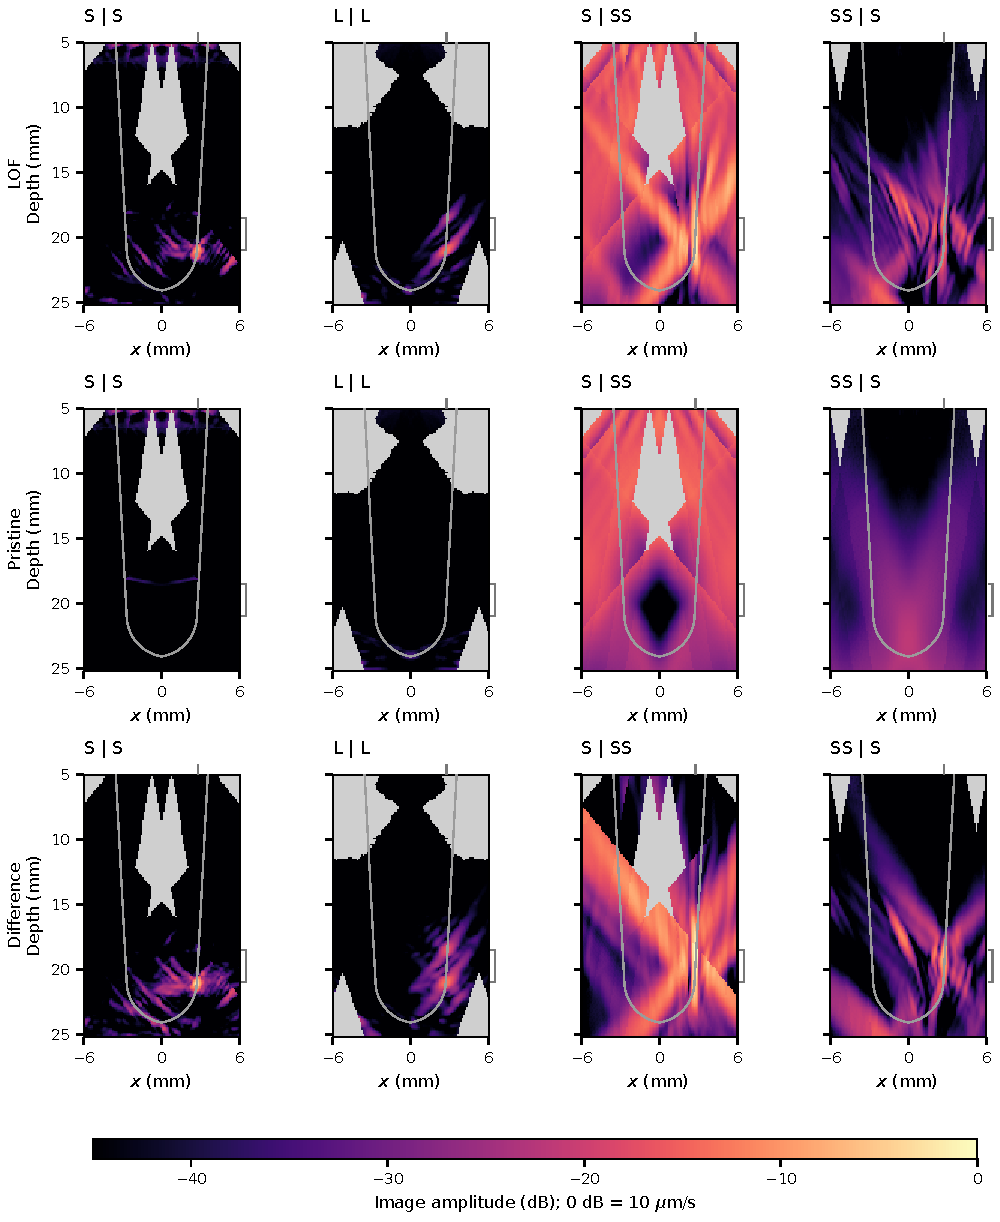
\includegraphics[width=\linewidth]{figures/saft_appendix/comsol/full_case_atlas.pdf}
\caption{All four full-weld paths at 0.1 mm spacing under the common 0.5--5 MHz protocol. Rows show LOF, pristine and signed-waveform-difference reconstructions. All panels share a 10 $\mu$m/s reference and 45 dB range; grey is unsupported. External LOF guides indicate a coordinate on pristine panels, whose models contain no flaw.}
\label{saftapp:archive:full:atlas}
\end{figure}
All four LOF-only maxima lie within 0.37 mm of the prescribed segment. Direct S and L emphasize the lower-tip vicinity; reflected shear views give broader and less selective indications. Near support is 100\% in each full-weld field. Table~\ref{saftapp:archive:full:controls} retains the complete three-case numerical comparison independently of display clipping.

\begin{table}[htbp]\centering\small
\caption{Common-protocol controls at 0.1 mm. $I_{\rm pk}$ is global peak velocity score; $d_{\rm pk}$ is distance from the finite prescribed LOF. N denotes near-flaw support.}
\label{saftapp:archive:full:controls}
\begin{tabular}{@{}llrrrrr@{}}\toprule
Path & Case & $I_{\rm pk}$ ($\mu$m/s) & $C_{\max}$ (dB) & $C_{99}$ (dB) & N (\%) & $d_{\rm pk}$ (mm)\\\midrule
$S\mid S$ & LOF & 4.347 & 6.47 & 15.57 & 100.0 & 0.004 \\
$S\mid S$ & Pristine & 2.061 & -21.39 & -10.22 & 100.0 & 13.805 \\
$S\mid S$ & Difference & 8.304 & 16.13 & 22.48 & 100.0 & 0.133 \\
\addlinespace
$L\mid L$ & LOF & 2.081 & 8.85 & 19.11 & 100.0 & 0.095 \\
$L\mid L$ & Pristine & 0.343 & -21.94 & -12.20 & 100.0 & 7.508 \\
$L\mid L$ & Difference & 2.220 & 9.10 & 15.14 & 100.0 & 0.033 \\
\addlinespace
$S\mid SS$ & LOF & 8.731 & 4.65 & 7.64 & 100.0 & 0.080 \\
$S\mid SS$ & Pristine & 2.320 & -4.38 & -3.04 & 100.0 & 13.175 \\
$S\mid SS$ & Difference & 18.451 & 8.34 & 14.16 & 100.0 & 0.269 \\
\addlinespace
$SS\mid S$ & LOF & 3.957 & 4.37 & 8.27 & 100.0 & 0.369 \\
$SS\mid S$ & Pristine & 0.840 & -6.52 & -5.82 & 100.0 & 3.321 \\
$SS\mid S$ & Difference & 4.707 & 4.49 & 11.08 & 100.0 & 0.030 \\
\addlinespace

\bottomrule\end{tabular}
\end{table}

The pristine and difference panels help distinguish structural response from changes caused by the flaw. They do not establish that pristine subtraction would be available in a real inspection. Different source means, cancellation and qualification can move the peak after subtraction. A blend of paths is a useful display of complementary responses; it is not a statistically justified fusion score or a direct measurement of LOF length.

See the shared filter definitions and variants in Section~\ref{saftapp:archive:shared:filter_details}.
\subsection{Complete filter/path outcomes}
\begin{figure}[!htbp]\centering
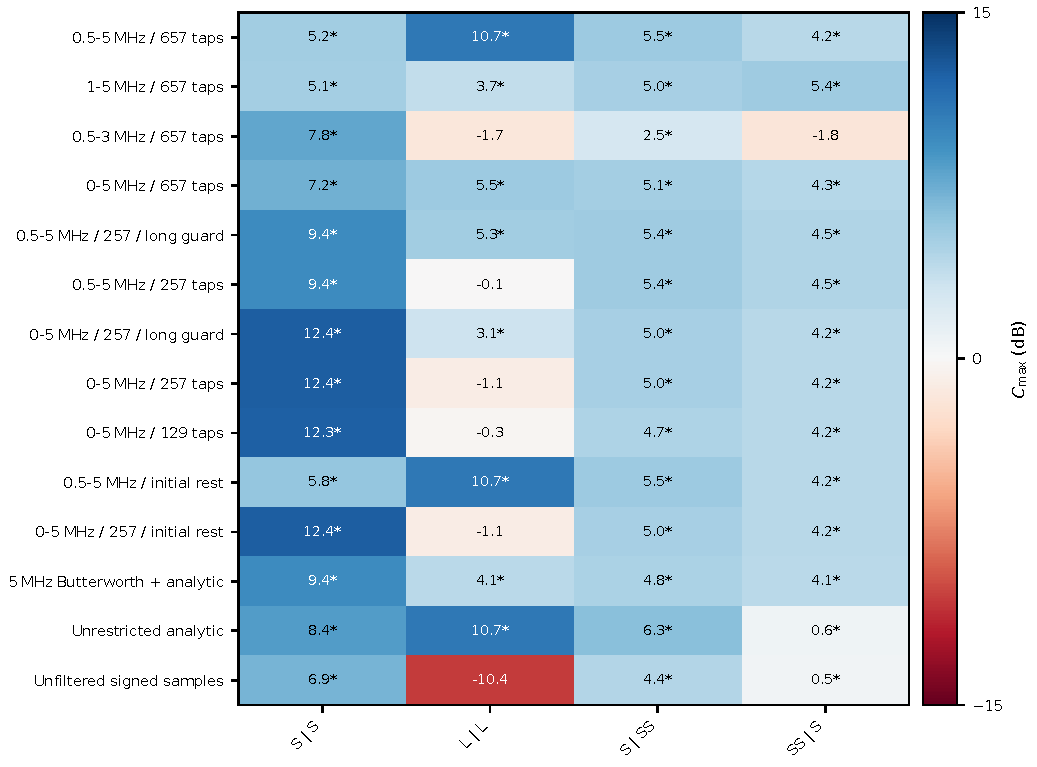
\includegraphics[width=\linewidth]{figures/saft_appendix/comsol/full_filter_matrix_0.pdf}
\caption{All fourteen processing variants for the four full-weld paths at 0.2 mm spacing. Entries are LOF-only $C_{\max}$ in dB; asterisks mark global maxima within 0.5 mm of the flaw. Colours saturate at $\pm15$ dB but values and arrays remain untruncated. The survey grid is coarser than the confirmation tables.}
\label{saftapp:archive:full:matrix}
\end{figure}
The ranking is path dependent. At 0.1 mm, direct-S contrast rises from 6.47 dB for the common bandpass to 10.26 dB for the shorter bandpass with matched guard, then 12.79 dB for the shorter low-pass with that guard. The improvement depends on both shorter temporal averaging and retained low-frequency content. It is not caused by admitting earlier times. Direct L instead falls from 8.85 to 3.24 dB under the same shorter low-pass, so a universal filter replacement is unsupported.

\subsection{Explicit full-weld delays and background coincidences}
For surface coordinate $q$ and pixel $p=(x,z)$, define $d(q,p)=\sqrt{(x-q)^2+z^2}$ and $b(q,p)=\sqrt{(x-q)^2+(2h-z)^2}$, with $h=25.4$ mm. The four delays are
\begin{align}
 T_{S\mid S}&=t_0+[d(x_s,p)+d(x_r,p)]/c_S,&
 T_{L\mid L}&=t_0+[d(x_s,p)+d(x_r,p)]/c_L,\\
 T_{S\mid SS}&=t_0+[d(x_s,p)+b(x_r,p)]/c_S,&
 T_{SS\mid S}&=t_0+[b(x_s,p)+d(x_r,p)]/c_S.
\end{align}
The reflected branches enforce specular same-mode reflection at the backwall. A near-vertical embedded separation is not generally specular for a top-to-flaw-to-top route; tip-associated scattering can dominate the direct image. Backwall-assisted illumination motivates tandem views~\cite{nicolson23}, but a bright reflected arc need not be a mapped flaw face.

All 1685 source--receiver pairs have unobstructed direct-family geometry for nuisance prediction. This does not isolate their measured modes. The recordings contain much stronger source-generated bulk/surface packets and boundary returns. For a symmetric pair separated by $d$, a direct nuisance wave of speed $c_n$ can coincide with a direct imaging hypothesis of speed $c_i>c_n$ at
\begin{equation}
 z_{\rm ghost}=\frac d2\sqrt{(c_i/c_n)^2-1}.
\end{equation}
With $d=20$ mm, L focusing can map direct S motion to about 15.4 mm depth, while S focusing can map Rayleigh motion to about 4.1 mm. Finite pulses broaden these loci. A 5 mm grid minimum or a near-source receiver exclusion therefore cannot guarantee clean deeper images.

\subsection{Complete confirmation register}
Table~\ref{saftapp:archive:full:register} lists every finer/wider, group and gate confirmation, including pristine and difference contrasts. Short names refer to the filter definitions above. Grid entries are pixel spacing in mm; ``wide'' changes the field to $x=\pm45$ mm. All other unlisted controls remain those of the stated protocol. Missing contrasts remain undefined. The portable arrays retain support, coherence and screened fractions for all three cases.
{\small\setlength{\tabcolsep}{4pt}
\singlespacing
\begin{longtable}{@{}llrlrrrr@{}}
\caption{Complete full-weld confirmations. BP denotes 0.5--5 MHz and LP 0--5 MHz; G328 retains the 3.28 $\mu$s guard. Rest uses known zero prehistory. L/P/D are LOF, pristine and difference $C_{\max}$ in dB; N is LOF near support. Src/rx denote source/receiver group reductions; weld and side identify the weld surface and side surfaces.}\label{saftapp:archive:full:register}\\
\toprule Filter & Path & Grid & Change & L & P & D & N (\%)\\\midrule\endfirsthead
\multicolumn{8}{l}{\small Continued from previous page}\\\toprule Filter & Path & Grid & Change & L & P & D & N (\%)\\\midrule\endhead
\bottomrule\endfoot
BP657 & $L\mid L$ & 0.1 & weld src & -- & -- & -- & 0.0 \\
BP657 & $L\mid L$ & 0.1 & all & 8.85 & -21.94 & 9.10 & 100.0 \\
BP657 & $L\mid L$ & 0.1 & weld rx & -11.77 & -31.02 & -5.63 & 100.0 \\
BP657 & $L\mid L$ & 0.1 & side rx & 6.43 & -23.43 & 7.70 & 100.0 \\
BP657 & $L\mid L$ & 0.1 & shoulder src & 8.85 & -21.94 & 9.10 & 100.0 \\
BP657 & $L\mid L$ & 0.1 & shoulder+side & 6.43 & -23.43 & 7.70 & 100.0 \\
BP657 & $L\mid L$ & 0.25 & wide & 6.90 & -29.50 & 8.70 & 100.0 \\
BP657 & $S\mid S$ & 0.1 & weld src & -51.58 & -47.53 & -47.87 & 9.8 \\
BP657 & $S\mid S$ & 0.1 & all & 6.47 & -21.39 & 16.13 & 100.0 \\
BP657 & $S\mid S$ & 0.05 & all & 6.63 & -21.26 & 16.13 & 100.0 \\
BP657 & $S\mid S$ & 0.1 & weld rx & -2.72 & -0.27 & 2.73 & 92.4 \\
BP657 & $S\mid S$ & 0.1 & side rx & 4.01 & -23.52 & 15.00 & 100.0 \\
BP657 & $S\mid S$ & 0.1 & shoulder src & 8.05 & -7.91 & 13.64 & 92.4 \\
BP657 & $S\mid S$ & 0.1 & shoulder+side & 7.19 & -7.28 & 12.38 & 92.4 \\
BP657 & $S\mid S$ & 0.25 & wide & 3.22 & -28.90 & 10.29 & 100.0 \\
BP657 & $S\mid SS$ & 0.1 & weld src & -14.43 & -9.48 & -8.64 & 9.8 \\
BP657 & $S\mid SS$ & 0.1 & all & 4.65 & -4.38 & 8.34 & 100.0 \\
BP657 & $S\mid SS$ & 0.1 & weld rx & -- & -- & -- & 0.0 \\
BP657 & $S\mid SS$ & 0.1 & side rx & 4.84 & -4.18 & 8.37 & 100.0 \\
BP657 & $S\mid SS$ & 0.1 & shoulder src & 5.28 & -2.04 & 9.24 & 92.4 \\
BP657 & $S\mid SS$ & 0.1 & shoulder+side & 5.28 & -1.53 & 8.82 & 92.4 \\
BP657 & $S\mid SS$ & 0.25 & wide & 4.88 & -5.31 & 8.07 & 100.0 \\
BP657 & $SS\mid S$ & 0.1 & weld src & -- & -- & -- & 0.0 \\
BP657 & $SS\mid S$ & 0.1 & all & 4.37 & -6.52 & 4.49 & 100.0 \\
BP657 & $SS\mid S$ & 0.1 & weld rx & -2.47 & -0.43 & -0.24 & 100.0 \\
BP657 & $SS\mid S$ & 0.1 & side rx & 4.92 & -6.82 & 4.41 & 100.0 \\
BP657 & $SS\mid S$ & 0.1 & shoulder src & 4.37 & -6.52 & 4.49 & 100.0 \\
BP657 & $SS\mid S$ & 0.1 & shoulder+side & 4.92 & -6.82 & 4.41 & 100.0 \\
BP657 & $SS\mid S$ & 0.25 & wide & -17.80 & -36.66 & -6.98 & 100.0 \\
BP257/G328 & $L\mid L$ & 0.1 & all & 4.96 & -34.09 & 8.40 & 100.0 \\
BP257/G328 & $S\mid S$ & 0.1 & all & 10.26 & -10.37 & 16.04 & 100.0 \\
BP257/G328 & $S\mid SS$ & 0.1 & all & 4.80 & -4.57 & 8.26 & 100.0 \\
BP257/G328 & $SS\mid S$ & 0.1 & all & 4.65 & -6.46 & 4.61 & 100.0 \\
LP257/G328 & $L\mid L$ & 0.1 & all & 3.24 & -36.97 & 5.97 & 100.0 \\
LP257/G328 & $S\mid S$ & 0.1 & all & 12.79 & -5.90 & 16.84 & 100.0 \\
LP257/G328 & $S\mid S$ & 0.05 & all & 12.63 & -6.57 & 16.68 & 100.0 \\
LP257/G328 & $S\mid SS$ & 0.1 & all & 4.97 & -3.75 & 8.58 & 100.0 \\
LP257/G328 & $SS\mid S$ & 0.1 & all & 4.32 & -6.00 & 4.65 & 100.0 \\
LP257/G328 & $S\mid S$ & 0.1 & all & 12.79 & -5.90 & 16.84 & 100.0 \\
LP257/G328 & $S\mid S$ & 0.1 & weld src & -20.66 & -19.08 & -38.32 & 9.8 \\
LP257/G328 & $S\mid S$ & 0.1 & weld rx & -2.64 & -0.32 & 2.72 & 92.4 \\
LP257/G328 & $S\mid S$ & 0.1 & gate 15\% & 10.16 & -4.12 & 15.10 & 100.0 \\
LP257/G328 & $S\mid S$ & 0.1 & gate 25\% & 13.79 & -14.49 & 17.40 & 100.0 \\
LP257/G328 & $S\mid S$ & 0.1 & LP launch & 12.79 & -5.90 & 16.84 & 100.0 \\
LP257/G328 & $S\mid S$ & 0.1 & side rx & 11.83 & -5.27 & 15.60 & 100.0 \\
LP257/G328 & $S\mid S$ & 0.1 & shoulder src & 10.57 & -4.14 & 14.23 & 92.4 \\
LP257/G328 & $S\mid S$ & 0.1 & shoulder+side & 9.61 & -3.51 & 12.99 & 92.4 \\
LP257/G328 & $S\mid S$ & 0.25 & wide & 10.62 & -20.09 & 10.83 & 100.0 \\
\end{longtable}}


\section{Partial weld: original path comparison}
\label{saftapp:partial}
\label{saftapp:archive:partial:principal}
\subsection{Direct S illumination with a reflected S return}
The selected hypothesis is $S\mid SS$: one S leg from source to trial pixel, followed by an S return through one backwall reflection. Weld-surface sources can illuminate the lower weld without traversing the empty groove. The reflected receiving branch reaches a side surface with a different angle and later arrival than a direct branch. The worked example illustrates why this can be geometrically useful, while the following images test whether the actual scattered field supports it.

The conventional catalogue contains eight pure-S splits, eight pure-L splits and the direct conversion hypotheses $L\mid S$ and $S\mid L$. All use the same common 657-tap 0.5--5 MHz filter and declared selection rules. Some hypotheses are weak, some are contaminated, and some have insufficient support. Their complete images remain in Section~\ref{saftapp:archive:partial:catalogue}; showing only the selected path without those controls would overstate general success.

\subsection{What is available from all five source shots?}
\begin{figure}[!htbp]\centering
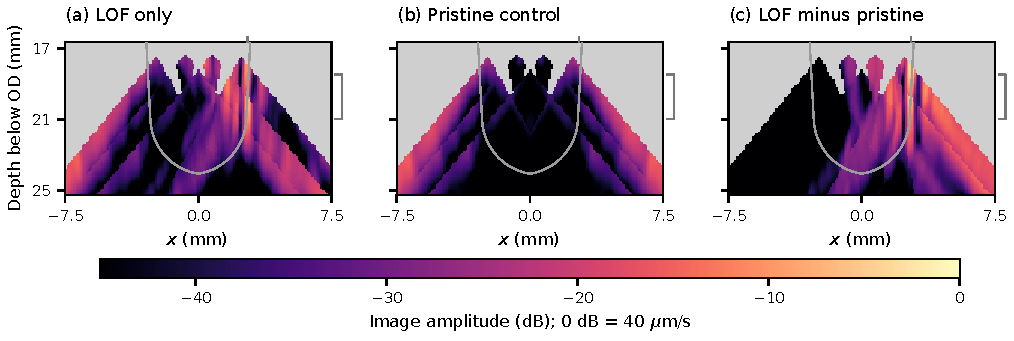
\includegraphics[width=\linewidth]{figures/saft_appendix/comsol/primary_partial.pdf}
\caption{All-source/all-receiver $S\mid SS$ reconstruction at 0.1 mm spacing, with pristine and waveform-difference controls. All panels use 0 dB = 40 $\mu$m/s over 45 dB. The first grid centre is 0.25 mm below the weld surface. Grey represents failure of the coverage rules, not zero recorded velocity. External marks indicate the prescribed separation without covering the reconstructed response.}
\label{saftapp:archive:partial:selected}
\end{figure}

With all sources and receivers, the LOF-only global maximum is 16.568 $\mu$m/s at $(2.8,19.95)$ mm, 0.0458 mm from the prescribed segment. Maximum-background contrast is 4.36 dB, percentile contrast is 8.74 dB and near-flaw support is 95.8\%. The near-flaw maximum therefore exceeds the strongest distant supported response, although the separation is less pronounced than a high-contrast isolated target might suggest.

The pristine control peaks at 6.820 $\mu$m/s at $(-6.9,23.25)$ mm. The waveform difference peaks at 32.743 $\mu$m/s at $(2.8,18.05)$ mm and has 11.09 dB contrast. The contrast and position changes demonstrate that introducing the LOF affects the measured field. They do not mean that the difference panel measures an additional flaw, or that a pristine reference must be used in the LOF-only reconstruction. Different signed interference and coherence after subtraction can move and strengthen the maximum.


\section{Partial weld: original source and receiver comparisons}
\label{saftapp:archive:partial:acquisition_results}
\subsection{What whole-group tests reveal}
The source and receiver play different physical roles. A weld-surface source can illuminate the lower weld directly, while a receiver on that same surface may encounter short-time contamination or an unfavourable return angle. A useful source position therefore need not be a useful receiving location for the same path.

\begin{table}[!htbp]\centering\small
\caption{Separate source or receiver group changes for $S\mid SS$, with the common processing and 0.1 mm grid. A dash denotes no near-flaw support under the declared qualification rules.}
\begin{tabularx}{\linewidth}{@{}Xrr@{}}\toprule
Acquisition & $C_{\max}$ (dB) & Near support (\%)\\\midrule
All sources and receivers & 4.36 & 95.8 \\
Shoulder sources only & -- & 0.0 \\
Weld-surface sources only & 8.77 & 48.5 \\
Side-surface receivers only & 4.33 & 95.8 \\
Weld-surface receivers only & -4.82 & 95.8 \\
Shoulders and side-surface receivers & -- & 0.0 \\

\bottomrule\end{tabularx}
\label{saftapp:archive:partial:groups}
\end{table}

Shoulder generation alone provides no near-flaw image under the two-source qualification rule. This means insufficient admitted evidence for an image; it does not mean that the shoulder sources launch no flaw-interacting waves. Using only the three weld-surface sources with all receivers gives 8.77 dB contrast but 48.5\% near support. The all-source case has lower contrast but substantially broader support. Complementary source shots therefore remain useful even when their addition lowers a local contrast metric.

Keeping all sources and receiving only on the two side surfaces gives 4.33 dB and 95.8\% near support, close to the all-receiver result. Receiving only on the weld surface instead gives negative maximum-background contrast despite high support. These comparisons motivate the joint combination of weld-surface generation and side-surface reception. They also explain why simply placing every optical measurement on the nearest available surface is not sufficient.

\subsection{Left, right or both receiving sides?}
\label{saftapp:archive:partial:joint}
The joint comparison fixes all three weld-surface sources S1--S3 and tests both side receiver groups, the left group alone and the right group alone. Each side has 157 positions at 0.25 mm pitch. The filter, path, thresholds and pixel spacing remain fixed. No individual receiver IDs are fitted to the known LOF.

\begin{figure}[!htbp]\centering
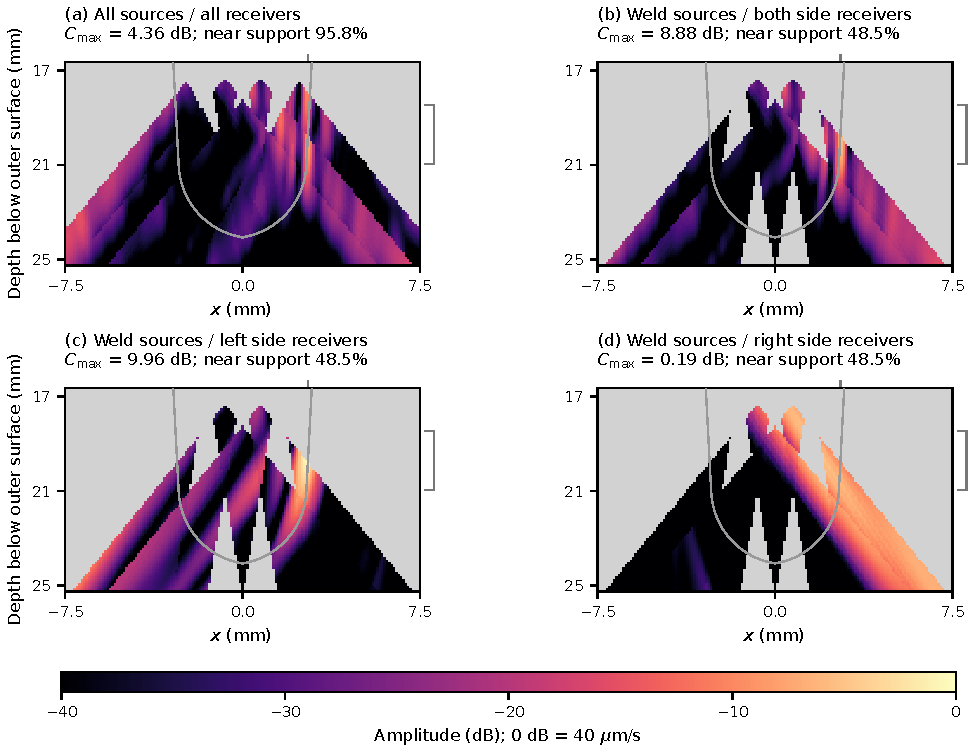
\includegraphics[width=\linewidth]{figures/saft_appendix/comsol/partial_joint.pdf}
\caption{Joint acquisition comparison for $S\mid SS$ with a shared 40 $\mu$m/s reference over 40 dB. The all-source image is compared with three weld-surface-source images using both, left or right side receivers. The clearer left-side indication comes with reduced coverage relative to the all-source image. Compare both the coloured response and the grey unsupported region.}
\label{saftapp:archive:partial:joint_figure}
\end{figure}

\begin{table}[!htbp]\centering\small
\caption{Joint acquisition metrics at 0.1 mm. $C_{\rm own}$ evaluates each image's supported field; $C_{\rm shared}$ uses their identical common supported subset. N denotes near-flaw support and $d_{\rm pk}$ the global-peak distance from the finite LOF.}
\begin{tabularx}{\linewidth}{@{}Xrrrr@{}}\toprule
Acquisition & $C_{\rm own}$ & N & $C_{\rm shared}$ & $d_{\rm pk}$\\
 & dB & \% & dB & mm\\\midrule
All sources / all receivers & 4.36 & 95.8 & 7.02 & 0.046 \\
Weld sources / both side surfaces & 8.88 & 48.5 & 8.88 & 0.046 \\
Weld sources / left side surface & 9.96 & 48.5 & 9.96 & 0.065 \\
Weld sources / right side surface & 0.19 & 48.5 & 0.19 & 0.664 \\

\bottomrule\end{tabularx}
\label{saftapp:archive:partial:joint_table}
\end{table}

Left-side reception gives 9.96 dB contrast and a global peak of 37.21 $\mu$m/s at $(2.7,19.75)$ mm, 0.065 mm from the prescribed segment. Both sides together give 8.88 dB. Right-side reception alone gives only 0.19 dB, with its global maximum 0.664 mm from the segment, outside the 0.5 mm near-flaw region. Left-side reception is therefore a useful reduced localizing view for this right-flank LOF and this path.

The improvement over both sides is 1.09 dB, not an order-of-magnitude change. Its physical plausibility comes from directional scattering and interference: the two sides observe different angles and different structural returns. Adding the second side can reduce coherent reinforcement of the useful signal or add coherent background. The present comparison does not uniquely separate those mechanisms, and it does not establish that left-side reception is best for a left-flank flaw or a different path.

\subsection{The coverage cost must remain part of the result}
All three weld-source acquisitions have the same supported pixels and only 48.5\% near-flaw support. The all-source/all-receiver image supports 95.8\%. Thus the 9.96 dB left-side score cannot be compared uncritically with the all-source 4.36 dB score: the latter also assesses a larger background and near-flaw region.

On the common supported set, the all-source result is 7.02 dB. The corresponding left-side advantage is 2.94 dB. This comparison isolates the change in reconstructed amplitude/background from the loss of available evidence. It still does not restore coverage to the omitted region. Figure~\ref{saftapp:archive:partial:coverage_map} displays that distinction directly.

\begin{figure}[!htbp]\centering
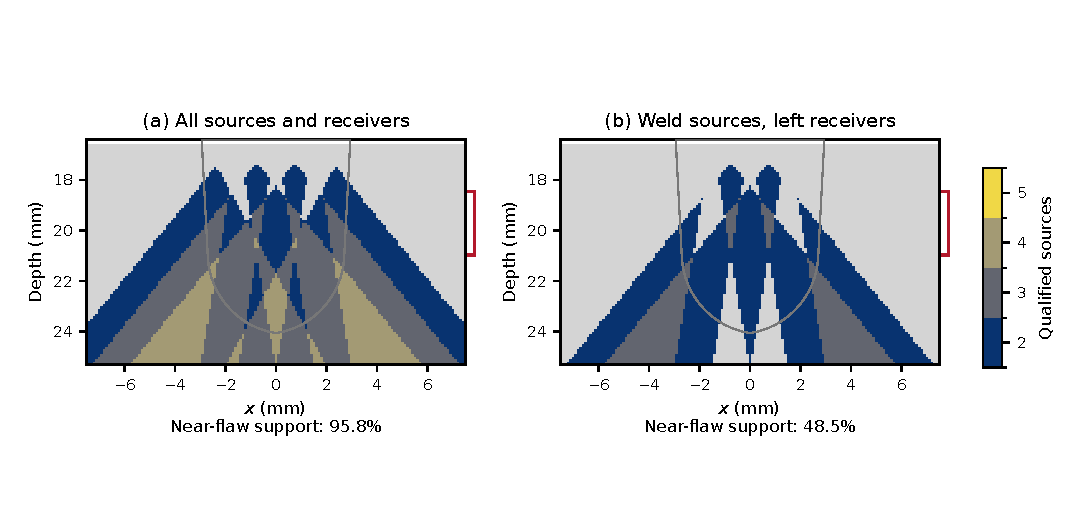
\includegraphics[width=.92\linewidth]{figures/saft_appendix/explanatory/partial_coverage.pdf}
\caption{Number of qualifying source views at each supported pixel for the all-source acquisition and the weld-source/left-receiver acquisition. The grey region has fewer than the required two qualified sources; white is air. Each qualified source separately satisfies the receiver-count and retained-fraction rules. This is a coverage map, not an amplitude image. Near-flaw support of 95.8\% and 48.5\% refers to area within 0.5 mm of the finite LOF, not the fraction of its length detected.}
\label{saftapp:archive:partial:coverage_map}
\end{figure}

For the left-side acquisition, the pristine contrast is $-33.09$ dB and the waveform-difference contrast is 9.86 dB. Both-side reception gives $-10.36$ and 7.95 dB for the corresponding controls. These support a flaw-related indication without introducing reference subtraction into the LOF-only image. They do not turn an unsupported region into an inspected region.


\section{Partial weld: original sensitivity checks}
\label{saftapp:archive:partial:sensitivity}
\subsection{Finer pixels and a wider field}
At 0.05 mm spacing, left-side reception gives 10.26 dB and both-side reception 8.59 dB, with 47.8\% near support. On the wider field at 0.25 mm spacing, they give 9.11 and 9.20 dB, with 43.4\% near support and near-flaw global maxima. The useful localization survives both checks. The left-side contrast advantage does not persist in every field, so a universal claim of superiority would be too strong.

The all-source acquisition gives 4.36 dB at 0.05 mm and 6.43 dB in the wider field, with near-flaw maxima. These are separate coverage-rich controls. Their contrasts cannot be interpreted as gains from changing pixel size alone, because the evaluated background field and discrete support also change.

\begin{figure}[!htbp]\centering
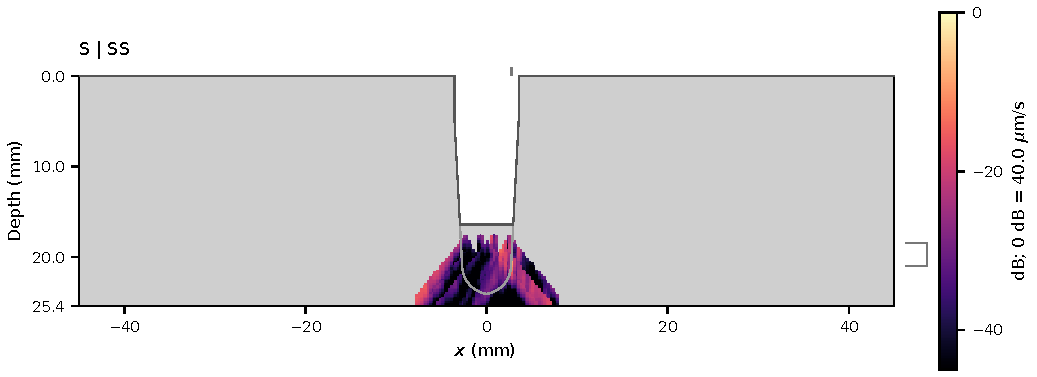
\includegraphics[width=\linewidth]{figures/saft_appendix/comsol/partial_wide.pdf}
\caption{All-source $S\mid SS$ control over the wider field at 0.25 mm spacing. The common reference is 40 $\mu$m/s over 45 dB. White identifies the empty groove, grey unsupported steel. This confirms a near-flaw global supported maximum for the broader-coverage acquisition; it does not imply inspection of every grey region.}
\label{saftapp:archive:partial:wide}
\end{figure}

\subsection{Filtering and additional paths}
For the all-source $S\mid SS$ confirmation, changing the common filter to 1--5 MHz gives 4.20 dB; shortening the 0.5--5 MHz kernel gives 4.29 dB; using the short 0--5 MHz low-pass gives 4.34 dB. The guard remains fixed and near support remains 95.8\%. These small changes support keeping the common bandpass for the partial-weld recipe. They are not a full filter optimization repeated for the one-sided acquisition.

The eighteen-path joint survey with weld-surface sources and both receiving sides has only one route with positive maximum-background contrast and a near-flaw global maximum: $S\mid SS$. The left-only acquisition is a subsequent comparison for this route, not a complete one-sided survey of all eighteen paths. This limits the claim to a justified selected view rather than the best possible path/side combination.

More complicated paths can sample strong reverberations, lose usable receivers or accumulate timing-model error. Separate finite-bevel and corner hypotheses were also investigated. None improved the evidence under the tested model; the corner extension assumed a unit diffraction amplitude and therefore cannot rule out a better physical diffraction model. The conventional reconstruction already rejects rays through the groove. Failure of an additional path is not evidence that geometry was ignored, or that the associated elastic wave does not exist.


\section{Partial weld: one-source and two-source requirements}
\label{saftapp:archive:partial:one_source}
\subsection{A coverage rule, not a choice of a single laser}
The minimum-source requirement applies separately at each pixel. Lowering it from two to one does not remove the other source shots: wherever two or three weld-surface sources qualify, their images are still combined exactly as before. It allows a pixel to be displayed when just one source has a sufficiently large, sufficiently coupled and sufficiently retained receiver aperture. The eight-receiver and 25\% retained-fraction thresholds remain in force, as do geometry, filtering, pulse screening and receiver coherence.

For a newly admitted pixel with only one qualified source, Equation~\ref{saftapp:source_rms} reduces to
\begin{equation}
 I_P(p)=|C_sM_s|,\qquad K=1.
\end{equation}
There is still coherent combination across receivers; what is missing is another qualifying source view. The nominal two-source rule is a corroboration and coverage safeguard, not an elastic-law prohibition against imaging with one shot.

\subsection{The controlled comparison}
The test changes only the required number of sources within each acquisition. It includes all-source/all-receiver, weld-source/both-side and weld-source/left-side configurations at 0.1 mm, a finer left-side grid and wider left/both-side fields. Every configuration has LOF, pristine and waveform-difference controls. Two native replays reproduce the two-source baselines.

\begin{table}[!htbp]\centering\small
\caption{One versus two required sources for partial-weld $S\mid SS$, at 0.1 mm with all other settings fixed. N is near-flaw support. Contrast uses each resulting supported field. All already-supported pixel amplitudes remain unchanged; newly admitted pixels have exactly one qualifying source.}
\begin{tabularx}{\linewidth}{@{}Xrrrr@{}}\toprule
Acquisition & Minimum & $C_{\max}$ & N & $d_{\rm pk}$\\
 & sources & dB & \% & mm\\\midrule
All sources / all receivers & 2 & 4.36 & 95.8 & 0.046 \\
All sources / all receivers & 1 & 2.15 & 100.0 & 0.046 \\
Weld sources / both sides & 2 & 8.88 & 48.5 & 0.046 \\
Weld sources / both sides & 1 & 3.06 & 95.8 & 0.046 \\
Weld sources / left side & 2 & 9.96 & 48.5 & 0.065 \\
Weld sources / left side & 1 & 3.72 & 95.8 & 0.325 \\

\bottomrule\end{tabularx}
\label{saftapp:archive:partial:source_threshold_table}
\end{table}

With weld-surface generation and left-side reception, near-flaw support rises from 48.5\% to 95.8\%. The indication is stronger in absolute amplitude, but background rises more: the peak becomes 46.15 $\mu$m/s, while the strongest distant background becomes 30.07 $\mu$m/s. Consequently, $C_{\max}$ falls from 9.96 to 3.72 dB. The global maximum moves from $(2.7,19.75)$ mm to $(2.9,18.15)$ mm, 0.325 mm from the finite prescribed segment and above its upper tip. It remains inside the declared 0.5 mm evaluation neighbourhood, but is no longer the same interior indication.

\begin{figure}[!htbp]\centering
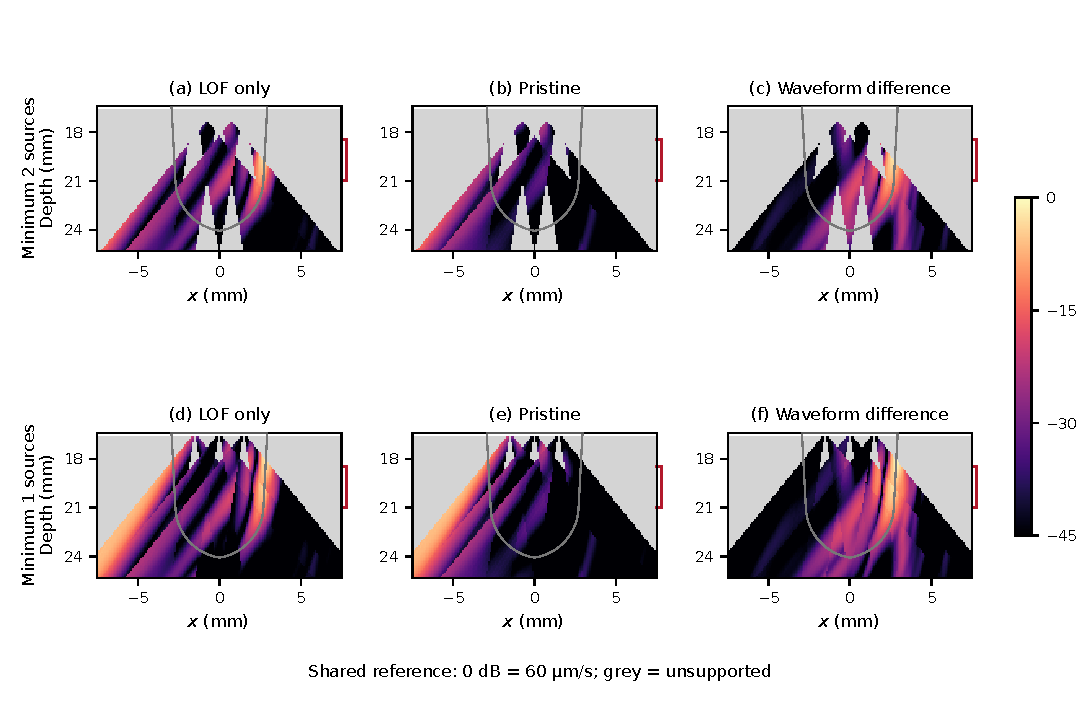
\includegraphics[width=\linewidth]{figures/saft_appendix/explanatory/partial_source_threshold.pdf}
\caption{Two-source and one-source admission for weld-surface generation and left-side reception. Columns show LOF-only, pristine and waveform-difference images. A shared 60 $\mu$m/s reference and 45 dB range keep every panel on the same amplitude scale without saturating the new peaks. Lowering the threshold fills previously grey pixels; it does not alter the values of the pixels already supported by two sources. The new regions include both a near-upper-tip response and substantial structural background.}
\label{saftapp:archive:partial:source_threshold_figure}
\end{figure}

With all sources and receivers, near-flaw support rises from 95.8\% to 100\%, while contrast falls from 4.36 to 2.15 dB. Its global peak and position remain unchanged. With the three weld-surface sources and both receiver sides, support rises from 48.5\% to 95.8\% and contrast falls from 8.88 to 3.06 dB, again without moving the global peak. Thus the large coverage recovery is especially relevant to weld-source-only imaging, but it is not a free gain in selectivity.

On the common supported pixels, every paired amplitude agrees with its two-source value within the numerical replay tolerance. The native checks also confirm unchanged source counts there, and exactly one source at every newly admitted pixel. This establishes the mechanism directly: the threshold changes which pixels are assessed, rather than changing the focusing operation at existing pixels. A matched-support contrast would therefore be unchanged and cannot by itself describe the value or risk of the recovered region.

\subsection{Do the new pixels behave like useful additional evidence?}
For the one-source left-side image, the pristine contrast is $-37.53$ dB and the difference contrast is 10.02 dB. The near-flaw response is therefore not accompanied by a comparably dominant pristine response at the same coordinates. However, the pristine image admits a 30.91 $\mu$m/s structural maximum elsewhere. This supports treating the recovered near-flaw response as informative while retaining the visible evidence of increased background.

At 0.05 mm spacing, one-source left reception gives 3.73 dB and 95.8\% near support. Over the wider field it gives 3.22 dB and 94.3\%, with a global maximum at $(2.75,18.0)$ mm, 0.475 mm from the LOF. Both-side reception over that wider field gives 4.87 dB with the same near support and a maximum only 0.012 mm from the segment. Thus the left-only preference is not universal when the qualification rule and assessed field change. The upper-end response also approaches the boundary of the declared near-flaw neighbourhood; it should not be described as a precisely located flaw tip.

The useful interpretation is to retain the two-source image as the cleaner localizing view and provide the one-source image as an explicitly marked broader-coverage view. One-source pixels have valid receiver support, but less source-view corroboration. This is more informative than either hiding all of them or presenting their expanded coverage as equally selective evidence. The test does not establish that a physically single-source inspection would reproduce the result, since the accepted source can differ from pixel to pixel.


\section{Partial weld: complete baseline comparisons}

\label{saftapp:archive:partial:complete}
The main findings above use the confirmed 0.1 mm results and selected finer/wider checks. This section supplies the full reproducible record: the eighteen-path catalogue and all signal controls at 0.2 mm, the fourteen processing variants and their matrices, additional geometric hypotheses, timing estimates and all confirmation configurations. A path comparison, a filter comparison and a change of image field answer different questions; their grids and controls are stated separately.

\subsection{Wall-response gate and source--receiver exclusion}
\label{saftapp:archive:partial:gate_audit}
The wall gate (5\%) and source--receiver exclusion (1.5 mm) are disabled separately and jointly, with all other controls fixed. The audit includes the common-band path surveys and all confirmations: 52 full-weld and 46 partial-weld configurations. Three perturbations per configuration and three signal cases give 294 reconstructions and 882 paired image comparisons. Repeating the principal nominal settings checks the archived arrays.

Image change is measured before display clipping, over the intersection $\Omega$ of supported pixels:
\begin{equation}
 \delta_I=100\frac{\lVert I_{\rm test}-I_{\rm nominal}\rVert_{2,\Omega}}
 {\lVert I_{\rm nominal}\rVert_{2,\Omega}}\ \%.
\end{equation}
Support changes are assessed separately. Table~\ref{saftapp:archive:partial:gate_controls} gives the principal LOF-only view; its support mask is identical in all four cases.

\begin{table}[htbp]\centering\small
\caption{Independent and joint gate checks for the principal
partial-weld $S\mid SS${}
image at 0.1 mm spacing. Zero disables the corresponding gate. $\delta_I$ measures whole-image amplitude change on common support; it is not a change in detection probability.}
\label{saftapp:archive:partial:gate_controls}
\begin{tabular}{@{}lrrr@{}}\toprule
Wall gate / exclusion & $C_{\max}$ (dB) & $\delta_I$ (\%) & Near support (\%)\\\midrule
5\% / 1.5 mm & 4.36 & 0.00 & 95.8 \\
0\% / 1.5 mm & 4.36 & 0.00 & 95.8 \\
5\% / 0 mm & 3.52 & 8.18 & 95.8 \\
0\% / 0 mm & 3.52 & 8.18 & 95.8 \\

\bottomrule\end{tabular}
\end{table}

Disabling the wall gate leaves the principal $S\mid SS$ image exactly unchanged. It is not redundant for the complete path family: on the 0.2 mm common-band grid, the LOF-only changes are 49.81\% for $S\mid SSS$, 7.73\% for $SS\mid SS$ and 39.84\% for $SS\mid SSS$. These routes have more intermediate reflections, and the gate acts on the product of their predicted coefficients. The percentages describe changes in the reconstructed field, not gains in flaw detection. The same nominal wall gate is retained throughout the family; it does not explain the principal indication.

Disabling the separation rule changes the principal image by 8.18\% and reduces $C_{\max}$ from 4.36 to 3.52 dB, with unchanged near support. Disabling both controls produces exactly the same principal image as disabling separation alone. The exclusion therefore has a measurable effect even though the focused flaw lies away from the source.

The 1.5 mm exclusion avoids the 1.425 mm effective source footprint, where directly applied loading complicates interpretation as a remotely received wave. It does not guarantee background removal. The exclusion distance and 5\% wall threshold are declared engineering safeguards; neither has been established as a universal optimum.

\subsection{The eighteen-path catalogue and all signal controls}\label{saftapp:archive:partial:catalogue}
For each pure mode M (L or S), the catalogue includes $M\mid M$, $M\mid MM$, $MM\mid M$, $M\mid MMM$, $MM\mid MM$, $MMM\mid M$, $MM\mid MMM$ and $MMM\mid MM$. In the four-leg split $MM\mid MM$, each branch has one backwall reflection. A three-leg branch has backwall and exposed-top reflections. The two direct conversion paths $L\mid S$ and $S\mid L$ complete the eighteen candidates. In the latter pair the mode changes at the pixel, not at a wall.

Figures~\ref{saftapp:archive:partial:lof_atlas}--\ref{saftapp:archive:partial:difference_atlas} show every primary path and signal case on the 0.2 mm survey grid using the same \saftappPartialDisplayReference\ $\mu$m/s reference and 55 dB range. The paired numerical table gives near amplitude, global-peak location relative to the flaw, contrast and support. A small supported region or a clean black image is not evidence of successful background elimination.

\begin{figure}[htbp]\centering
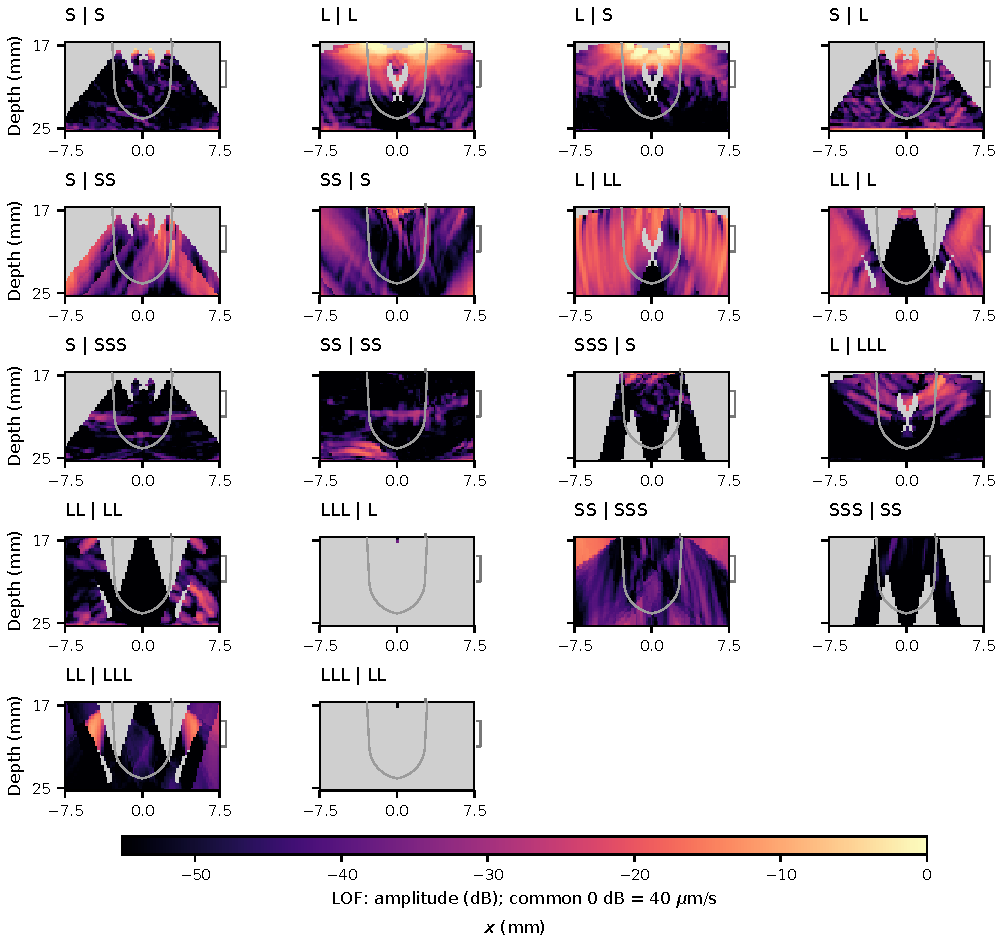
\includegraphics[width=\linewidth]{figures/saft_appendix/comsol/partial_lof_atlas.pdf}
\caption{All eighteen partial-weld LOF-only images under equal receiver averaging and the common bandpass, at 0.2 mm spacing. External marks locate the known flaw without covering the reconstructed signals. Air is white and unsupported material grey. Colour saturates above the common reference; numerical scores are untruncated.}
\label{saftapp:archive:partial:lof_atlas}
\end{figure}
\begin{figure}[htbp]\centering
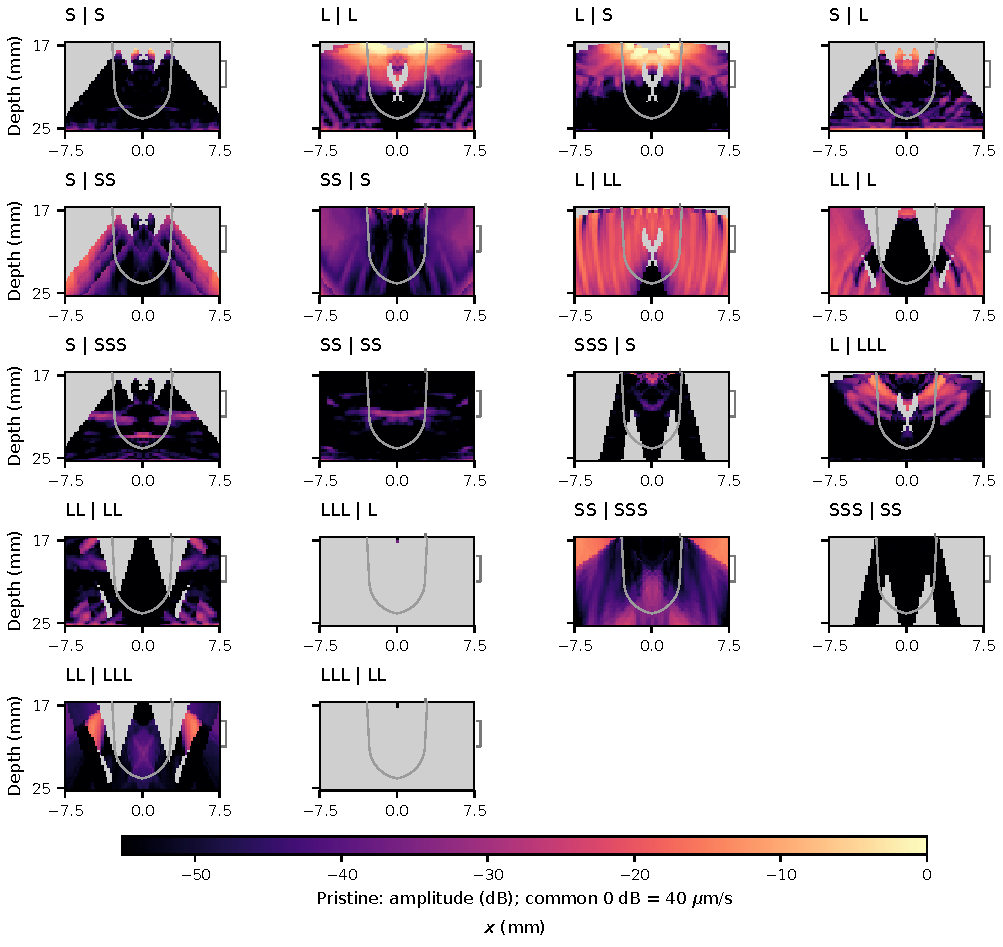
\includegraphics[width=\linewidth]{figures/saft_appendix/comsol/partial_reference_atlas.pdf}
\caption{All eighteen pristine-control images with the same controls, scale and grid as Figure~\ref{saftapp:archive:partial:lof_atlas}. The location marks are coordinate guides; these models contain no flaw. Structural response near the known LOF coordinates demonstrates why proximity alone is insufficient evidence.}
\label{saftapp:archive:partial:reference_atlas}
\end{figure}
\begin{figure}[htbp]\centering
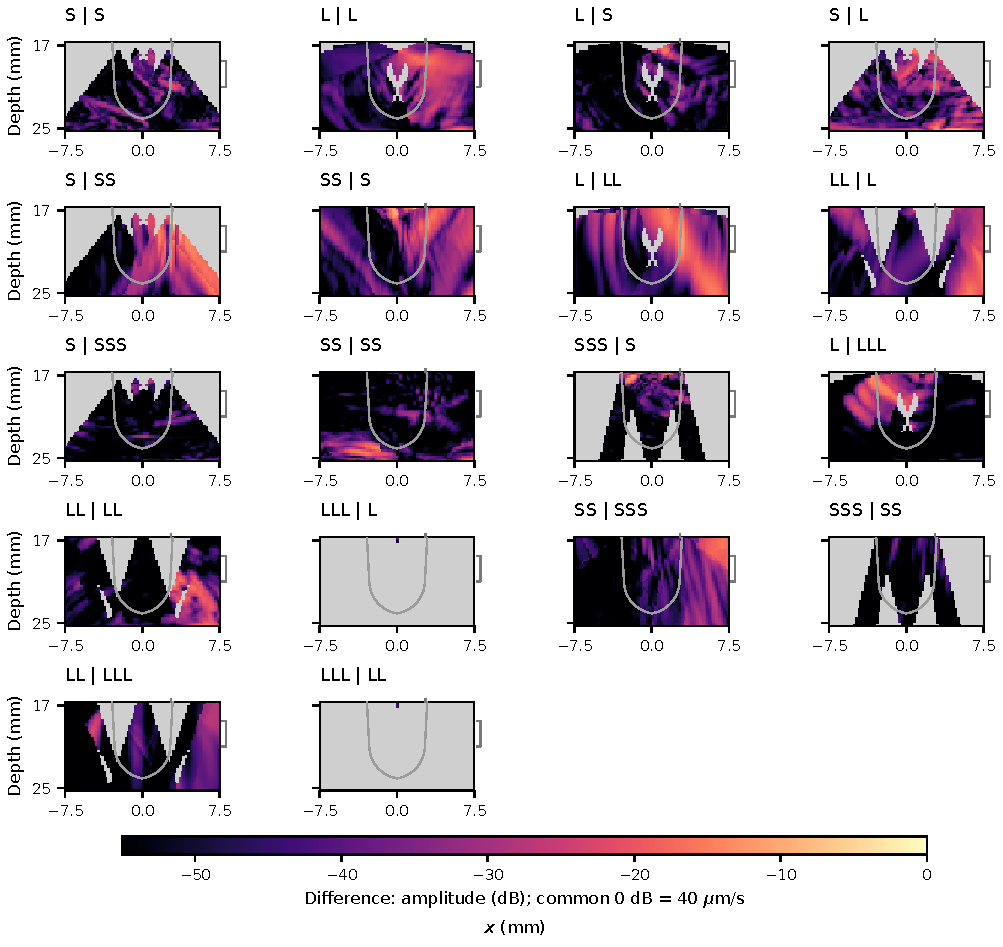
\includegraphics[width=\linewidth]{figures/saft_appendix/comsol/partial_difference_atlas.pdf}
\caption{All eighteen waveform-difference images on the same scale and grid. Signed waveforms are subtracted before nonlinear focusing. Changed reverberation and interference can contribute alongside direct flaw scattering. These are diagnostic controls, not the basis of the LOF-only screening procedure.}
\label{saftapp:archive:partial:difference_atlas}
\end{figure}
\FloatBarrier

{\small\setlength{\tabcolsep}{4pt}
\begin{longtable}{@{}llrrrrr@{}}
\caption{All eighteen primary partial-weld paths and three signal cases on the 0.2 mm survey grid. $I_N$ is the near-region maximum in $\mu$m/s; distances are mm and contrasts dB. N is near support.}\label{saftapp:archive:partial:primary_register}\\
\toprule Path & Case & $I_N$ & $C_{\max}$ & $C_{99}$ & N (\%) & $d_{\rm pk}$\\\midrule\endfirsthead
\multicolumn{7}{l}{\small Continued from previous page}\\\toprule Path & Case & $I_N$ & $C_{\max}$ & $C_{99}$ & N (\%) & $d_{\rm pk}$\\\midrule\endhead
\bottomrule\endfoot
$S\mid S$ & LOF & 1.74 & -24.13 & -7.86 & 95.2 & 2.362 \\
$S\mid S$ & Pristine & 0.54 & -33.23 & -15.28 & 95.2 & 2.362 \\
$S\mid S$ & Difference & 7.32 & 3.20 & 13.32 & 95.2 & 0.083 \\
\addlinespace
$L\mid L$ & LOF & 16.07 & -10.45 & -8.25 & 100.0 & 5.517 \\
$L\mid L$ & Pristine & 13.32 & -12.08 & -9.88 & 100.0 & 1.456 \\
$L\mid L$ & Difference & 6.46 & -0.65 & 3.72 & 100.0 & 5.468 \\
\addlinespace
$L\mid S$ & LOF & 11.16 & -15.99 & -13.87 & 100.0 & 4.016 \\
$L\mid S$ & Pristine & 10.89 & -16.36 & -14.36 & 100.0 & 1.839 \\
$L\mid S$ & Difference & 2.11 & -9.86 & -0.95 & 100.0 & 1.736 \\
\addlinespace
$S\mid L$ & LOF & 4.13 & -13.18 & -10.99 & 95.2 & 4.324 \\
$S\mid L$ & Pristine & 0.46 & -32.08 & -30.99 & 95.2 & 4.356 \\
$S\mid L$ & Difference & 6.52 & -7.42 & -1.39 & 95.2 & 4.645 \\
\addlinespace
$S\mid SS$ & LOF & 13.34 & 3.65 & 6.90 & 95.2 & 0.038 \\
$S\mid SS$ & Pristine & 3.04 & -7.01 & -5.78 & 95.2 & 9.868 \\
$S\mid SS$ & Difference & 24.90 & 8.95 & 10.15 & 95.2 & 0.438 \\
\addlinespace
$SS\mid S$ & LOF & 3.20 & -14.26 & -5.10 & 100.0 & 4.151 \\
$SS\mid S$ & Pristine & 0.42 & -24.39 & -16.89 & 100.0 & 4.698 \\
$SS\mid S$ & Difference & 9.24 & -8.07 & 3.45 & 100.0 & 3.972 \\
\addlinespace
$L\mid LL$ & LOF & 6.47 & -8.89 & -2.93 & 100.0 & 2.377 \\
$L\mid LL$ & Pristine & 4.96 & -13.61 & -5.45 & 100.0 & 3.450 \\
$L\mid LL$ & Difference & 12.46 & 4.17 & 5.11 & 100.0 & 0.049 \\
\addlinespace
$LL\mid L$ & LOF & 0.24 & -29.18 & -26.50 & 3.6 & 3.795 \\
$LL\mid L$ & Pristine & 0.07 & -40.03 & -35.42 & 3.6 & 3.795 \\
$LL\mid L$ & Difference & 0.40 & -26.68 & -24.48 & 3.6 & 5.314 \\
\addlinespace
$S\mid SSS$ & LOF & 0.92 & -6.84 & -2.50 & 95.2 & 6.807 \\
$S\mid SSS$ & Pristine & 1.04 & -10.34 & -5.14 & 95.2 & 3.211 \\
$S\mid SSS$ & Difference & 0.97 & -6.05 & 0.25 & 95.2 & 2.412 \\
\addlinespace
$SS\mid SS$ & LOF & 1.59 & -13.68 & -8.06 & 100.0 & 7.287 \\
$SS\mid SS$ & Pristine & 0.96 & -8.90 & -0.74 & 100.0 & 6.432 \\
$SS\mid SS$ & Difference & 1.82 & -12.75 & -9.02 & 100.0 & 5.538 \\
\addlinespace
$SSS\mid S$ & LOF & 2.30 & -21.57 & -8.88 & 100.0 & 4.332 \\
$SSS\mid S$ & Pristine & 0.10 & -38.91 & -29.62 & 100.0 & 1.867 \\
$SSS\mid S$ & Difference & 4.37 & -13.42 & -6.02 & 100.0 & 2.253 \\
\addlinespace
$L\mid LLL$ & LOF & 9.48 & -2.51 & 8.04 & 100.0 & 2.377 \\
$L\mid LLL$ & Pristine & 9.75 & -5.39 & 2.22 & 100.0 & 3.450 \\
$L\mid LLL$ & Difference & 0.15 & -35.86 & -33.18 & 100.0 & 6.252 \\
\addlinespace
$LL\mid LL$ & LOF & 0.88 & -16.36 & -12.55 & 3.6 & 2.370 \\
$LL\mid LL$ & Pristine & 0.01 & -49.55 & -46.53 & 3.6 & 8.378 \\
$LL\mid LL$ & Difference & 7.49 & 0.84 & 3.79 & 3.6 & 0.522 \\
\addlinespace
$LLL\mid L$ & LOF & -- & -- & -- & 0.0 & 3.621 \\
$LLL\mid L$ & Pristine & -- & -- & -- & 0.0 & 3.621 \\
$LLL\mid L$ & Difference & -- & -- & -- & 0.0 & 3.117 \\
\addlinespace
$SS\mid SSS$ & LOF & 0.79 & -20.47 & -19.62 & 100.0 & 9.637 \\
$SS\mid SSS$ & Pristine & 0.20 & -32.90 & -32.41 & 100.0 & 4.120 \\
$SS\mid SSS$ & Difference & 1.01 & -16.69 & -15.22 & 100.0 & 4.120 \\
\addlinespace
$SSS\mid SS$ & LOF & 0.31 & -3.53 & -1.73 & 100.0 & 4.376 \\
$SSS\mid SS$ & Pristine & 0.04 & -6.18 & -4.73 & 100.0 & 1.396 \\
$SSS\mid SS$ & Difference & 0.71 & -1.50 & 2.36 & 100.0 & 4.151 \\
\addlinespace
$LL\mid LLL$ & LOF & 0.04 & -48.78 & -46.00 & 3.6 & 7.670 \\
$LL\mid LLL$ & Pristine & 0.03 & -47.97 & -46.34 & 3.6 & 2.096 \\
$LL\mid LLL$ & Difference & 0.05 & -36.01 & -32.18 & 3.6 & 7.481 \\
\addlinespace
$LLL\mid LL$ & LOF & -- & -- & -- & 0.0 & 3.257 \\
$LLL\mid LL$ & Pristine & -- & -- & -- & 0.0 & 3.450 \\
$LLL\mid LL$ & Difference & -- & -- & -- & 0.0 & 3.621 \\
\addlinespace
\end{longtable}}

See the shared filter definitions and variants in Section~\ref{saftapp:archive:shared:filter_details}.
\subsection{Complete filter/path comparison matrices}
Figures~\ref{saftapp:archive:partial:s_matrix} and~\ref{saftapp:archive:partial:l_matrix} retain the full survey, including negative contrasts and unsupported routes. The common 0.2 mm grid isolates processing comparisons from a change in spatial sampling. The asterisk distinguishes a near-flaw global maximum from a positive contrast whose global maximum falls in the excluded guard region. The finer-grid conclusions appear in Section~\ref{saftapp:archive:partial:sensitivity}; the complete confirmation register follows below.

On this survey grid, unrestricted analytic processing gives $S\mid SS$ 2.85 dB contrast, whereas signed unfiltered summation gives $-0.14$ dB and its global maximum lies outside the 0.5 mm near-flaw region. The five-leg $SSS\mid SS$ route gives weak positive contrasts of 1.59 and 1.18 dB for those respective controls. These outcomes show that changing the retained spectrum and phase representation can change the path ranking. They do not validate high-frequency propagation or establish a stronger alternative to the band-limited $S\mid SS$ result.
\begin{figure}[p]\centering
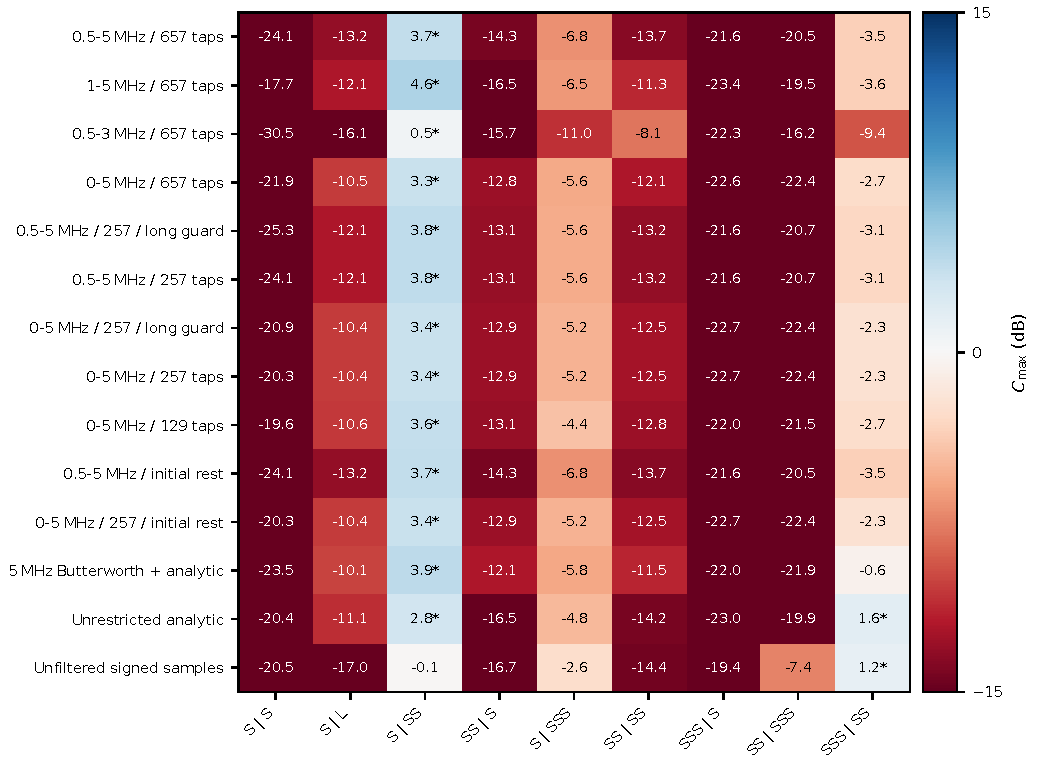
\includegraphics[width=\linewidth]{figures/saft_appendix/comsol/partial_filter_matrix_0.pdf}
\caption{All fourteen processing variants for incident-S partial-weld hypotheses at 0.2 mm spacing. Entries are LOF-only $C_{\max}$ in dB; an asterisk denotes a global maximum within 0.5 mm of the finite flaw. Colours saturate at $\pm15$ dB, without truncating the printed values. Undefined contrast is shown by a dash.}
\label{saftapp:archive:partial:s_matrix}
\end{figure}
\begin{figure}[p]\centering
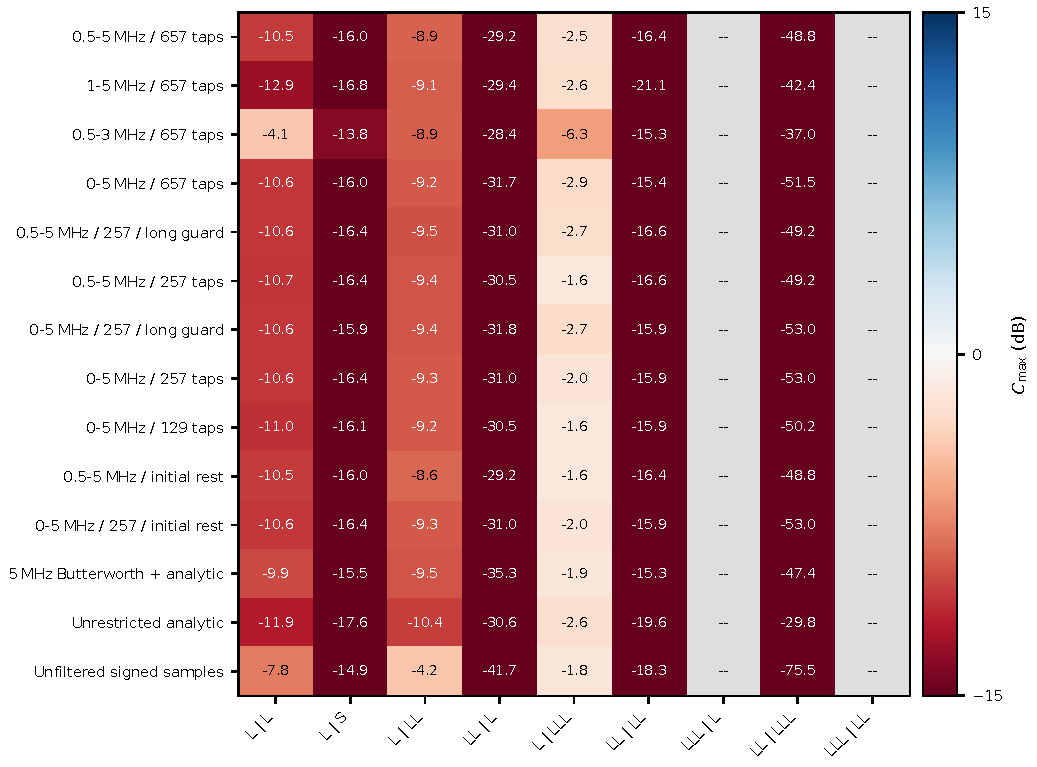
\includegraphics[width=\linewidth]{figures/saft_appendix/comsol/partial_filter_matrix_1.pdf}
\caption{Corresponding incident-L hypotheses under the same conventions. The signed unfiltered row changes signal representation as well as bandwidth; it is a diagnostic control rather than an envelope-equivalent reconstruction.}
\label{saftapp:archive:partial:l_matrix}
\end{figure}
\FloatBarrier
\subsection{Additional bevel and corner hypotheses}\label{saftapp:archive:partial:extensions}
Conventional imaging is geometry aware: actual endpoint heights set delays, finite exposed surfaces constrain reflections, and rays through the open groove are rejected. An additional catalogue tests 48 finite-bevel specular routes and 144 fixed-corner timing routes with equal receiver averaging at 0.2 mm spacing; six conventional controls use 0.1 mm spacing. Of the additional routes, 16 bevel and 60 corner paths have any supported pixels; only three bevel and 44 corner routes reach any near-flaw support. None places its global LOF-only maximum within 0.5 mm of the flaw or produces positive maximum-background contrast. Their failure therefore does not depend on ranking small differences against the finer-grid conventional control.

These negative outcomes describe the original equal-mean acquisition. The expanded weighted group survey in Section~\ref{saftapp:expanded_review} identifies useful corner-timing views under different controls, while retaining their calibration limitations. The extension used a unit corner-diffraction coefficient without a calibrated elastic amplitude or phase. Its negative result concerns those declared models, not every possible diffracted-wave method. Adding many geometric routes can create more opportunities to focus structural packets. Their inclusion in a colour blend would conceal this weakness unless each route's support and pristine control were first examined. The extension protocol, complete path metrics and verification summaries remain in the evidence archive.

\subsection{Timing estimates and limits of direct-arrival screening}
The LOF lies 2.0675--4.5675 mm below the floor. A floor-to-flaw echo may overlap local source motion or occur before the centred filter has complete support. For an illustrative colocated vertical pair, $T=t_0+2d/c_m$; the 3.28 $\mu$s guard gives $d_S\ge5.262$ mm or $d_L\ge9.658$ mm. The corresponding absolute depths are 21.662 and 26.058 mm. This is an explanation of the early-time problem, not a universal grid minimum: the actual protocol excludes colocated pairs and includes longer bistatic/reflected routes.

A floor--backwall round trip adds $2(9~\mathrm{mm})/c_S=5.559$ $\mu$s or $2(9~\mathrm{mm})/c_L=3.028$ $\mu$s. Such delays can move a desired echo into usable time support, but add reverberation and competing paths. Known zero prehistory supplies missing filter input before the initial time; it does not remove a physical source packet overlapping a flaw echo. These are distinct mechanisms.

Only 365 of the 1655 source--receiver pairs have unobstructed direct-family geometry for L/S/R nuisance screening: $2\times157$ shoulder/side-surface pairs and $3\times17$ weld-surface pairs. A Rayleigh guide requires a common unobstructed flat surface; it does not propagate a fictitious straight surface wave through the groove or around a corner. Unscreened reflections and diffraction can remain in every recording. Strong coherent background can survive receiver coherence and focus into arcs at pixels unrelated to the flaw.

\subsection{Complete confirmation register}
The following register includes all 28 confirmation configurations and their LOF, pristine and difference contrasts. Grid entries are spacing in mm; wide fields use $x=\pm45$ mm. All other settings follow the named protocol and the stated acquisition reduction.
{\small\setlength{\tabcolsep}{4pt}
\begin{longtable}{@{}llrlrrrr@{}}
\caption{Complete partial-weld confirmations. BP denotes 0.5--5 MHz and LP 0--5 MHz; G328 retains the 3.28 $\mu$s guard. Rest uses known zero prehistory. L/P/D are LOF, pristine and difference $C_{\max}$ in dB; N is LOF near support. Src/rx denote source/receiver group reductions; weld and side identify the weld surface and side surfaces.}\label{saftapp:archive:partial:register}\\
\toprule Filter & Path & Grid & Change & L & P & D & N (\%)\\\midrule\endfirsthead
\multicolumn{8}{l}{\small Continued from previous page}\\\toprule Filter & Path & Grid & Change & L & P & D & N (\%)\\\midrule\endhead
\bottomrule\endfoot
1--5/657 & $L\mid L$ & 0.1 & all & -13.03 & -14.27 & -0.77 & 100.0 \\
1--5/657 & $S\mid S$ & 0.1 & all & -16.88 & -29.25 & 2.28 & 95.8 \\
1--5/657 & $S\mid SS$ & 0.1 & all & 4.20 & -6.31 & 10.65 & 95.8 \\
1--5/657 & $SSS\mid SS$ & 0.1 & all & -3.82 & -6.04 & -2.33 & 100.0 \\
BP657 & $L\mid L$ & 0.1 & all & -10.60 & -12.23 & -0.65 & 100.0 \\
BP657 & $S\mid S$ & 0.1 & all & -25.54 & -35.30 & 2.54 & 95.8 \\
BP657 & $S\mid SS$ & 0.1 & weld src & 8.77 & -9.91 & 8.08 & 48.5 \\
BP657 & $S\mid SS$ & 0.1 & all & 4.36 & -6.87 & 11.09 & 95.8 \\
BP657 & $S\mid SS$ & 0.05 & all & 4.36 & -6.48 & 11.21 & 95.8 \\
BP657 & $S\mid SS$ & 0.1 & weld rx & -4.82 & -2.68 & 1.38 & 95.8 \\
BP657 & $S\mid SS$ & 0.1 & side rx & 4.33 & -7.27 & 11.34 & 95.8 \\
BP657 & $S\mid SS$ & 0.1 & shoulder src & -- & -- & -- & 0.0 \\
BP657 & $S\mid SS$ & 0.1 & shoulder+side & -- & -- & -- & 0.0 \\
BP657 & $S\mid SS$ & 0.25 & wide & 6.43 & -6.40 & 10.81 & 94.3 \\
BP657 & $SSS\mid SS$ & 0.1 & all & -4.02 & -5.88 & -0.94 & 100.0 \\
BP257/G328 & $L\mid L$ & 0.1 & all & -10.79 & -12.40 & -0.52 & 100.0 \\
BP257/G328 & $S\mid S$ & 0.1 & all & -27.18 & -40.58 & 2.51 & 95.8 \\
BP257/G328 & $S\mid SS$ & 0.1 & all & 4.29 & -6.58 & 11.18 & 95.8 \\
BP257/G328 & $SSS\mid SS$ & 0.1 & all & -3.87 & -6.62 & -1.22 & 100.0 \\
LP257/rest & $L\mid L$ & 0.1 & all & -10.68 & -11.79 & -1.16 & 100.0 \\
LP257/rest & $S\mid S$ & 0.1 & all & -22.18 & -47.73 & 3.08 & 95.8 \\
LP257/rest & $S\mid SS$ & 0.1 & all & 4.34 & -5.70 & 11.33 & 95.8 \\
LP257/rest & $SSS\mid SS$ & 0.1 & all & -2.72 & -1.68 & -1.07 & 100.0 \\
LP257/G328 & $L\mid L$ & 0.1 & all & -10.68 & -11.79 & -1.40 & 100.0 \\
LP257/G328 & $S\mid S$ & 0.1 & all & -22.69 & -47.74 & 2.94 & 95.8 \\
LP257/G328 & $S\mid SS$ & 0.1 & all & 4.34 & -5.70 & 11.33 & 95.8 \\
LP257/G328 & $S\mid SS$ & 0.05 & all & 4.32 & -5.29 & 11.42 & 95.8 \\
LP257/G328 & $SSS\mid SS$ & 0.1 & all & -2.72 & -1.68 & -1.07 & 100.0 \\
\end{longtable}}

\subsection{Joint-acquisition path survey and confirmation register}
The joint acquisition uses the three weld-surface sources and both side receiver groups for an eighteen-path survey at 0.2 mm spacing. Only $S\mid SS$ gives positive LOF-only maximum-background contrast with a global maximum inside the 0.5 mm near-flaw region. Its 7.63 dB contrast and 50.6\% near support motivate the 0.1 mm receiving-side comparison. The left/right test is therefore conditional on this path; it is not an exhaustive search over every path-specific one-sided aperture.

\begin{table}[htbp]\centering\small
\caption{All eighteen joint-acquisition paths at 0.2 mm spacing, with fixed common-bandpass processing. Contrasts are in dB; N is LOF-only near support (\%). A dash denotes undefined contrast because a required supported region is absent.}
\label{saftapp:archive:partial:joint_paths}
\begin{tabular}{@{}lrrrr@{}}\toprule
Path & LOF & Pristine & Difference & N\\\midrule
$S\mid S$ & -24.94 & -50.90 & 1.77 & 50.6 \\
$L\mid L$ & -9.21 & -10.83 & -0.41 & 100.0 \\
$L\mid S$ & -14.74 & -15.11 & -8.10 & 100.0 \\
$S\mid L$ & -19.85 & -40.11 & -9.19 & 50.6 \\
$S\mid SS$ & 7.63 & -11.22 & 7.71 & 50.6 \\
$SS\mid S$ & -13.52 & -15.50 & 0.72 & 86.7 \\
$L\mid LL$ & -7.64 & -11.73 & 5.41 & 100.0 \\
$LL\mid L$ & -- & -- & -- & 0.0 \\
$S\mid SSS$ & -13.72 & -34.14 & -4.92 & 50.6 \\
$SS\mid SS$ & -38.18 & -43.07 & -37.83 & 86.7 \\
$SSS\mid S$ & -- & -- & -- & 0.0 \\
$L\mid LLL$ & -0.74 & -3.58 & -38.88 & 100.0 \\
$LL\mid LL$ & -- & -- & -- & 0.0 \\
$LLL\mid L$ & -- & -- & -- & 0.0 \\
$SS\mid SSS$ & -21.14 & -34.18 & -14.15 & 86.7 \\
$SSS\mid SS$ & -- & -- & -- & 0.0 \\
$LL\mid LLL$ & -- & -- & -- & 0.0 \\
$LLL\mid LL$ & -- & -- & -- & 0.0 \\

\bottomrule\end{tabular}
\end{table}

\begin{table}[htbp]\centering\small
\caption{Joint-acquisition confirmation controls for $S\mid SS$. Every row uses weld-surface generation. The first three rows use the standard 0.1 mm grid; ``finer'' is 0.05 mm and ``wide'' is $x=\pm45$ mm, $z=0.25$--25.25 mm at 0.25 mm. Contrast columns are in dB, and N is LOF-only near support (\%).}
\label{saftapp:archive:partial:joint_controls}
\begin{tabularx}{\linewidth}{@{}Xrrrr@{}}\toprule
Receiving aperture / grid & LOF & Pristine & Difference & N\\\midrule
Both sides / 0.1 mm & 8.88 & -10.36 & 7.95 & 48.5 \\
Left side / 0.1 mm & 9.96 & -33.09 & 9.86 & 48.5 \\
Right side / 0.1 mm & 0.19 & -8.53 & -4.48 & 48.5 \\
Left side / finer & 10.26 & -33.09 & 10.14 & 47.8 \\
Left side / wide & 9.11 & -43.74 & 10.38 & 43.4 \\
Both sides / finer & 8.59 & -10.60 & 7.99 & 47.8 \\
Both sides / wide & 9.20 & -12.24 & 6.93 & 43.4 \\

\bottomrule\end{tabularx}
\end{table}

The eighteen survey, three receiving-side and four finer/wider configurations form 25 scientific comparisons. One additional all-source native replay reproduces the existing 0.1 mm arrays in all three signal cases, with identical source counts and amplitude agreement within $2\times10^{-9}$ relative tolerance ($10^{-15}$ m\,s$^{-1}$ absolute allowance). All 78 signal-case metrics are independently recomputed from the archived arrays. The protocol and loadable left-side settings accompany the evidence; no additional COMSOL solve is required.
\FloatBarrier

\subsection{Complete one-source requirement controls}
The source-requirement audit adds six scientific configurations and two
two-source numerical replays, separate from the primary and joint-acquisition
counts above. Each has three signal cases. All 24 paired checks confirm
unchanged amplitudes and source counts on previously supported pixels, within
$2\times10^{-9}$ relative and $10^{-15}$ m\,s$^{-1}$ absolute replay allowances.
All newly supported pixels have exactly one qualifying source. The audit
changes no filter, receiver threshold, gate or physical acquisition group
within a pair.
\begin{table}[!htbp]\centering\small
\caption{Complete one-source requirement controls. Standard grids use 0.1 mm,
finer grids 0.05 mm, and wide fields 0.25 mm over $x=\pm45$ mm and
$z=0.25$--25.25 mm. Contrasts use each image's full supported field; N is
LOF-only near-flaw support.}
\begin{tabularx}{\linewidth}{@{}Xrrrr@{}}\toprule
Acquisition / field & LOF & Pristine & Difference & N\\
 & dB & dB & dB & \%\\\midrule
All / standard & 2.15 & -10.11 & 9.38 & 100.0 \\
Weld, both / standard & 3.06 & -7.40 & 11.24 & 95.8 \\
Weld, left / standard & 3.72 & -37.53 & 10.02 & 95.8 \\
Weld, left / finer & 3.73 & -36.85 & 10.02 & 95.8 \\
Weld, left / wide & 3.22 & -42.78 & 9.50 & 94.3 \\
Weld, both / wide & 4.87 & -8.49 & 10.60 & 94.3 \\

\bottomrule\end{tabularx}
\end{table}
The reproducible protocol, arrays, metrics and loadable one-source left-side
settings are retained in the source-requirement audit folder. The two-source
settings remain available as the nominal comparison. No additional COMSOL
solve is needed for this qualification change.


\section{Partial weld: revised weighted result and grid checks}
\label{saftapp:updated}
\subsection{Reassessment: better contrast with broad near-flaw support}
\label{saftapp:review}
The preceding comparisons are the original equal-mean baseline. A broader review now tests response weighting, frequency band, angular and wall gates, source--receiver exclusion, direct and reflected screens, fixed mutes, coherence, receiver retention, source combination and acquisition groups. This appendix retains the complete comparisons. No new COMSOL solve is required: all changes reconstruct the same recorded wave fields.

For all five sources and all receivers, weighting alone improves the 0.1 mm common-band result from 4.36 to 8.05 dB with unchanged 95.8\% near support. A 1--5 MHz band gives 8.59 dB. Lowering the angular gate from 20\% to 15\% recovers a small additional region without accepting the large background introduced at 10\% or 5\%. With the 15\% gate and no fixed mute, the 0.025 mm result is 9.09 dB with 96.9\% near support.

Adding only the narrow backwall-$SS$ mute in Equation~\ref{saftapp:mute} raises that matched-grid contrast to 14.45 dB while retaining 96.9\% near support. The global peak is 58.64 $\mu$m/s at $(2.700,19.625)$ mm, 0.071 mm from the LOF. The pristine near-region maximum is 2.53 $\mu$m/s and its global maximum is elsewhere. The gain is not simply a reduction of every background value: muting also changes phase cancellation and coherence, and the largest background rises from 10.73 to 11.11 $\mu$m/s. The reconstructed near peak rises from 30.53 to 58.64 $\mu$m/s. These remain processed velocity scores, not a doubling of physical flaw-scattered energy.

\begin{figure}[!htbp]\centering
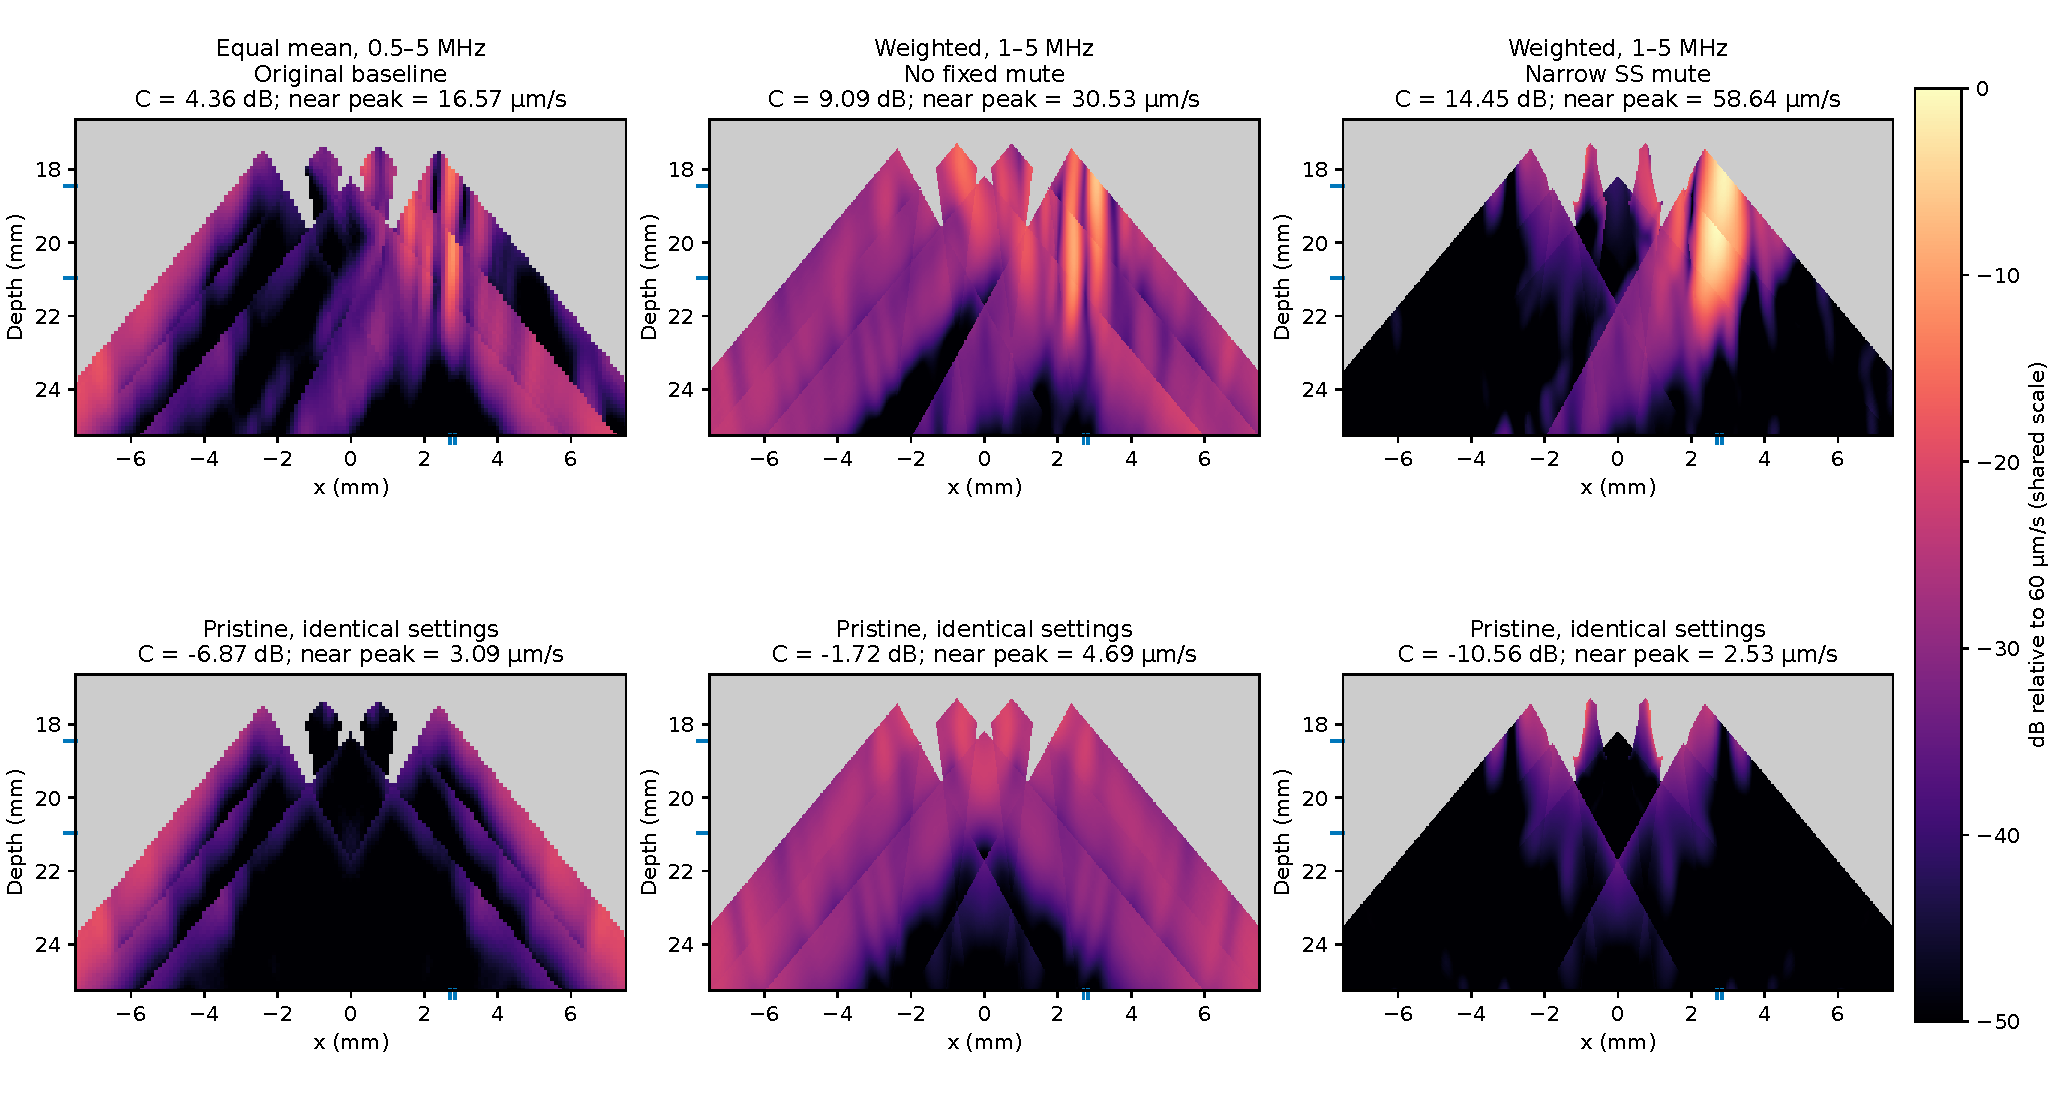
\includegraphics[width=\linewidth]{figures/saft_appendix/review/partial_reassessment.pdf}
\caption{Updated partial-weld $S\mid SS$ comparison. Columns show the original equal-mean baseline (0.1 mm), response weighting with 1--5 MHz and a 15\% angular gate (0.025 mm), and the same weighted recipe with the narrow $SS$ mute (0.025 mm). Rows show LOF-only and pristine controls on one absolute colour scale. Grey denotes unsupported material; external marks locate the prescribed segment. Only the last two columns form a matched-grid mute comparison.}
\label{saftapp:reassessment_image}
\end{figure}

The SAFT grid matters to peak-based scores. The muted result is 15.77 dB at 0.05 mm, but 14.45 dB at both 0.025 mm and a half-pixel-shifted 0.05 mm grid because those grids sample a stronger competing background peak. The more conservative 14.45 dB is therefore used here. The indication also survives the wider-field check, with its sampling stated in Table~\ref{saftapp:review_grid}. A finer image grid samples the focusing function more closely; it does not improve the finite-element solution or establish finer acoustic resolution.

\begin{table}[!htbp]\centering\small
\caption{Partial-weld grid checks. Local fields are $x=\pm7.5$ mm and depths 16.65--25.25 mm; wide fields are $x=\pm45$ mm and depths 0.25--25.25 mm. Entries state pixel spacing in mm. $d_{\rm pk}$ is the global-peak distance from the finite LOF. The shifted grid starts 0.025 mm later on both axes.}
\label{saftapp:review_grid}
\begin{tabular}{@{}lrrr@{}}\toprule
Recipe / grid & $C_{\max}$ (dB) & Near support (\%) & $d_{\rm pk}$ (mm)\\\midrule
Unmuted, 0.025 & 9.09 & 96.9 & 0.291\\
SS mute, 0.025 & 14.45 & 96.9 & 0.071\\
Unmuted, shifted 0.05 & 9.07 & 96.9 & 0.310\\
SS mute, shifted 0.05 & 14.45 & 96.9 & 0.099\\
SS mute, 0.05 & 15.77 & 96.8 & 0.070\\
SS mute, wide 0.25 & 16.18 & 96.2 & 0.015\\
SS mute, wide 0.1 & 15.77 & 96.7 & 0.070\\
\bottomrule\end{tabular}\end{table}

\subsection{What limits support, and do right-side paths help?}
The 25\% rule applies to each source's geometrically and angularly eligible aperture, not to all 331 receivers. A 600-combination audit of receiver fraction, actual/effective count and source minimum shows that the receiver thresholds do not limit either original all-aperture $S\mid SS$ anchor. Their least retained actual and effective counts are 224 and 189.1. Lowering those thresholds cannot recover channels that already failed visibility or angular admission. The remaining support loss chiefly reflects source geometry and launch sensitivity. At the 20\% gate, all 101 evaluated points on the exact LOF segment already have two-source support; missing pixels in its 0.5 mm neighbourhood do not imply an equally missing portion of flaw length. Allowing only one qualifying source fills that neighbourhood but admits more background.

Right-side receivers do contain useful information. A fixed shot at the right weld position S3, $(1.5,16.4)$ mm, with the 157 right receivers gives a useful $S\mid LL$ view: direct S illumination, conversion at the trial point and a backwall-reflected L return. At 0.05 mm it gives 3.02 dB unmuted, or 5.93 dB after a narrow predicted-$LL$ mute, with 96.8\% near support. This is a genuinely single-shot acquisition, unlike an image that permits one of several shots to qualify at each pixel. It is a complementary view rather than evidence that right reception is generally inferior to left reception.

Some longer paths look promising only in a small field. For example, left-weld S1 with right receivers and $SSL\mid SS$ gives 9.24 dB locally after raising the lower cutoff to 1.5 MHz, but $-25.24$ dB in the wider field, where its global maximum is 21.14 mm from the flaw. Rejecting full reflected-packet windows can instead remove all near support for $S\mid LL$. Useful local information, isolated physical-path identification and robust wide-field localization must therefore remain separate claims.

The extended review covers all 324 implemented path hypotheses, all seven nonempty physical receiver-group combinations and nine fixed source views. It also retains failures and pristine controls. Parameters were examined using this known flaw, so the revised recipe is a tested working choice for this dataset, not a validated optimum or a probability-of-detection result.

The wider search also finds useful reduced acquisitions beyond right-side reception. A single S3 shot with left receivers gives $S\mid SS$ 11.49 dB locally and 11.03 dB in the wider field, with approximately 96--97\% near support. S1 with left and weld-surface receivers gives $SLS\mid S$ 15.80 dB locally and 4.01 dB wider, with 98.6\% and 100\% support respectively. These values use 0.05 and 0.25 mm grids. Conversely, the initially highest-scoring $SLS\mid L$ view is nearly reproduced by the pristine specimen. Path, aperture, grid and pristine controls therefore all affect which indications are credible.


\section{Partial weld: expanded path and settings investigation}
\label{saftapp:expanded_review}
This section documents the review that changes the interpretation of the partial-weld result. The earlier equal-mean and reduced-aperture images remain valid baseline calculations. They do not exhaust the information in the recordings. In particular, the left-side preference was conditional on $S\mid SS$, its original filter and its selected source group. It cannot be generalized to every path or single weld-source shot.

\subsection{Declared search scope}
The broad path survey holds the weighted 1--5 MHz band, 15\% angular gate, 5\% wall gate, 1.5 mm source exclusion, direct L/S/R screens, CF exponent one and RMS source rule fixed. Its grid is 0.2 mm over $x=\pm7.5$ mm and depths 16.65--25.25 mm. Three disjoint receiver groups are exported separately for each of 324 paths: 132 conventional mode sequences, 48 finite-bevel reflection hypotheses and 144 fixed-corner timing hypotheses. The 972 native configurations each contain LOF, pristine and waveform-difference cases.

For each source, disjoint-group sums $Q_s$, $W_s$, $\sum w_{sr}^2$, $P_s$ and accepted/eligible counts are added \emph{before} evaluating coherence and qualification. Averaging already formed group images would be incorrect. All seven nonempty group combinations are evaluated with five single-source views, three weld sources requiring one or two, and all five sources requiring one or two. This gives 20,412 fixed acquisition/path views and 61,236 signal-case images. Every choice is fixed for the whole image; there is no pixelwise selection of the best path or brightest source.

The survey identifies 53 conventional paths (227 fixed views), 10 corner paths (61 fixed views), 0 wall paths (0 fixed views) with positive contrast, at least 20\% near support and a global maximum within 0.5 mm of the flaw. These are local-field screening results; they are not all independently confirmed candidates. The complete register below and CSV expose the acquisition choices and coverage behind each score.

\subsection{Following up the strongest path-survey indications}
Fifteen fixed views receive native 0.05 mm local and 0.25 mm wider-field checks. Selection includes high local scores, broad support, clear LOF/pristine separation and deliberately retained pristine lookalikes. Table~\ref{saftapp:path_confirmation} prevents the best coarse-grid score from becoming the conclusion without these checks.

\begingroup\small\setlength{\tabcolsep}{3pt}
\begin{longtable}{@{}>{\raggedright\arraybackslash}p{.34\linewidth}rrrrrr@{}}
\caption{All fifteen atlas follow-ups. Subscripts f/w mean 0.05 mm local / 0.25 mm wide field; $C$ is contrast (dB), $N$ near support (\%), $R_f$ the fine-grid LOF/pristine near-peak ratio (dB), and $d_w$ the wider-field global-peak distance (mm). A high $C$ with $R_f$ near zero can be a pristine lookalike.}\label{saftapp:path_confirmation}\\
\toprule Path; acquisition & $C_f$ & $N_f$ & $R_f$ & $C_w$ & $N_w$ & $d_w$\\\midrule\endfirsthead
\toprule Path; acquisition & $C_f$ & $N_f$ & $R_f$ & $C_w$ & $N_w$ & $d_w$\\\midrule\endhead
$SLS\mid L$; left/source1 & 15.83 & 76.3 & 0.36 & 1.58 & 73.6 & 0.50\\
$SLS\mid S$; left/source1 & 17.33 & 76.3 & -4.69 & -26.37 & 73.6 & 21.45\\
$LSS\mid LL$; left\_\allowbreak weld/source1 & 21.04 & 37.0 & 1.43 & -12.57 & 41.5 & 14.51\\
$LSS\mid L$; left\_\allowbreak weld/source1 & 19.98 & 37.0 & 0.32 & 0.32 & 41.5 & 0.24\\
$SSS\mid L$; left/weld\_\allowbreak min2 & 8.40 & 53.6 & 1.11 & -6.47 & 52.8 & 34.95\\
$LS\mid SL$; sides/source4 & 5.54 & 100.0 & 0.70 & 15.27 & 100.0 & 0.05\\
$LSS\mid S$; weld/source1 & 17.10 & 29.7 & 28.31 & 14.26 & 35.8 & 0.08\\
$SLL\mid S$; weld/source1 & 9.38 & 57.3 & 17.78 & 10.12 & 60.4 & 0.21\\
$SLS\mid S$; left\_\allowbreak weld/source1 & 15.80 & 98.6 & 28.48 & 4.01 & 100.0 & 0.08\\
$S\mid SS$; left/source3 & 11.49 & 96.8 & 50.09 & 11.03 & 96.2 & 0.27\\
$SL\mid SS$; sides/source4 & 7.27 & 100.0 & 15.94 & 3.60 & 100.0 & 0.53\\
$SS\mid S$; left\_\allowbreak weld/source1 & 3.78 & 99.0 & 35.22 & 3.62 & 100.0 & 0.33\\
$SL\mid S$; left\_\allowbreak weld/source4 & 7.15 & 100.0 & 23.77 & 3.74 & 100.0 & 0.18\\
Corner 5 L rx; right/source4 & 16.94 & 82.6 & 2.16 & -33.97 & 77.4 & 34.87\\
Corner 4 S tx; left\_\allowbreak weld/source0 & 6.19 & 100.0 & 22.82 & 7.90 & 100.0 & 0.18\\
\bottomrule\end{longtable}\endgroup

The largest coarse-grid score, S1 with left receivers and $SLS\mid L$, drops from 31.76 to 15.83 dB on the finer grid. Its near-flaw amplitude is only 0.36 dB above the pristine control, and the wide-field peak lies just outside the near region. It is not persuasive evidence of a uniquely flaw-generated indication. Likewise, S4 with both-side receivers and $LS\mid SL$ has 100\% near support but only 0.70 dB LOF/pristine separation on the fine grid. High localization contrast alone is insufficient when a similar response exists without a flaw.

There are useful alternatives. S3 with left receivers and unmuted $S\mid SS$ retains 11.49/11.03 dB in the fine/wide fields, approximately 96--97\% near support and about 50 dB LOF/pristine near-peak separation. S1 with left and weld receivers and $SLS\mid S$ gives 15.80/4.01 dB and 98.6/100\% support. The same source/group combination with $SS\mid S$ gives 3.78/3.62 dB and 99.0/100\% support. The latter views provide complementary information without declaring that the reconstructed delay uniquely identifies the scattered packet.

Some narrower views also survive the wider field: S1 with weld receivers gives $LSS\mid S$ 17.10/14.26 dB but only 29.7/35.8\% near support. A corner-timing route from S0 through corner 4 gives 6.19/7.90 dB with complete near support, but retains an uncalibrated corner scattering coefficient. It warrants further physical modeling rather than replacement of the conventional working recipe. None of the finite-bevel routes meets the survey's combined positive-contrast, local-peak and 20\% support criteria.

\begin{figure}[!htbp]\centering
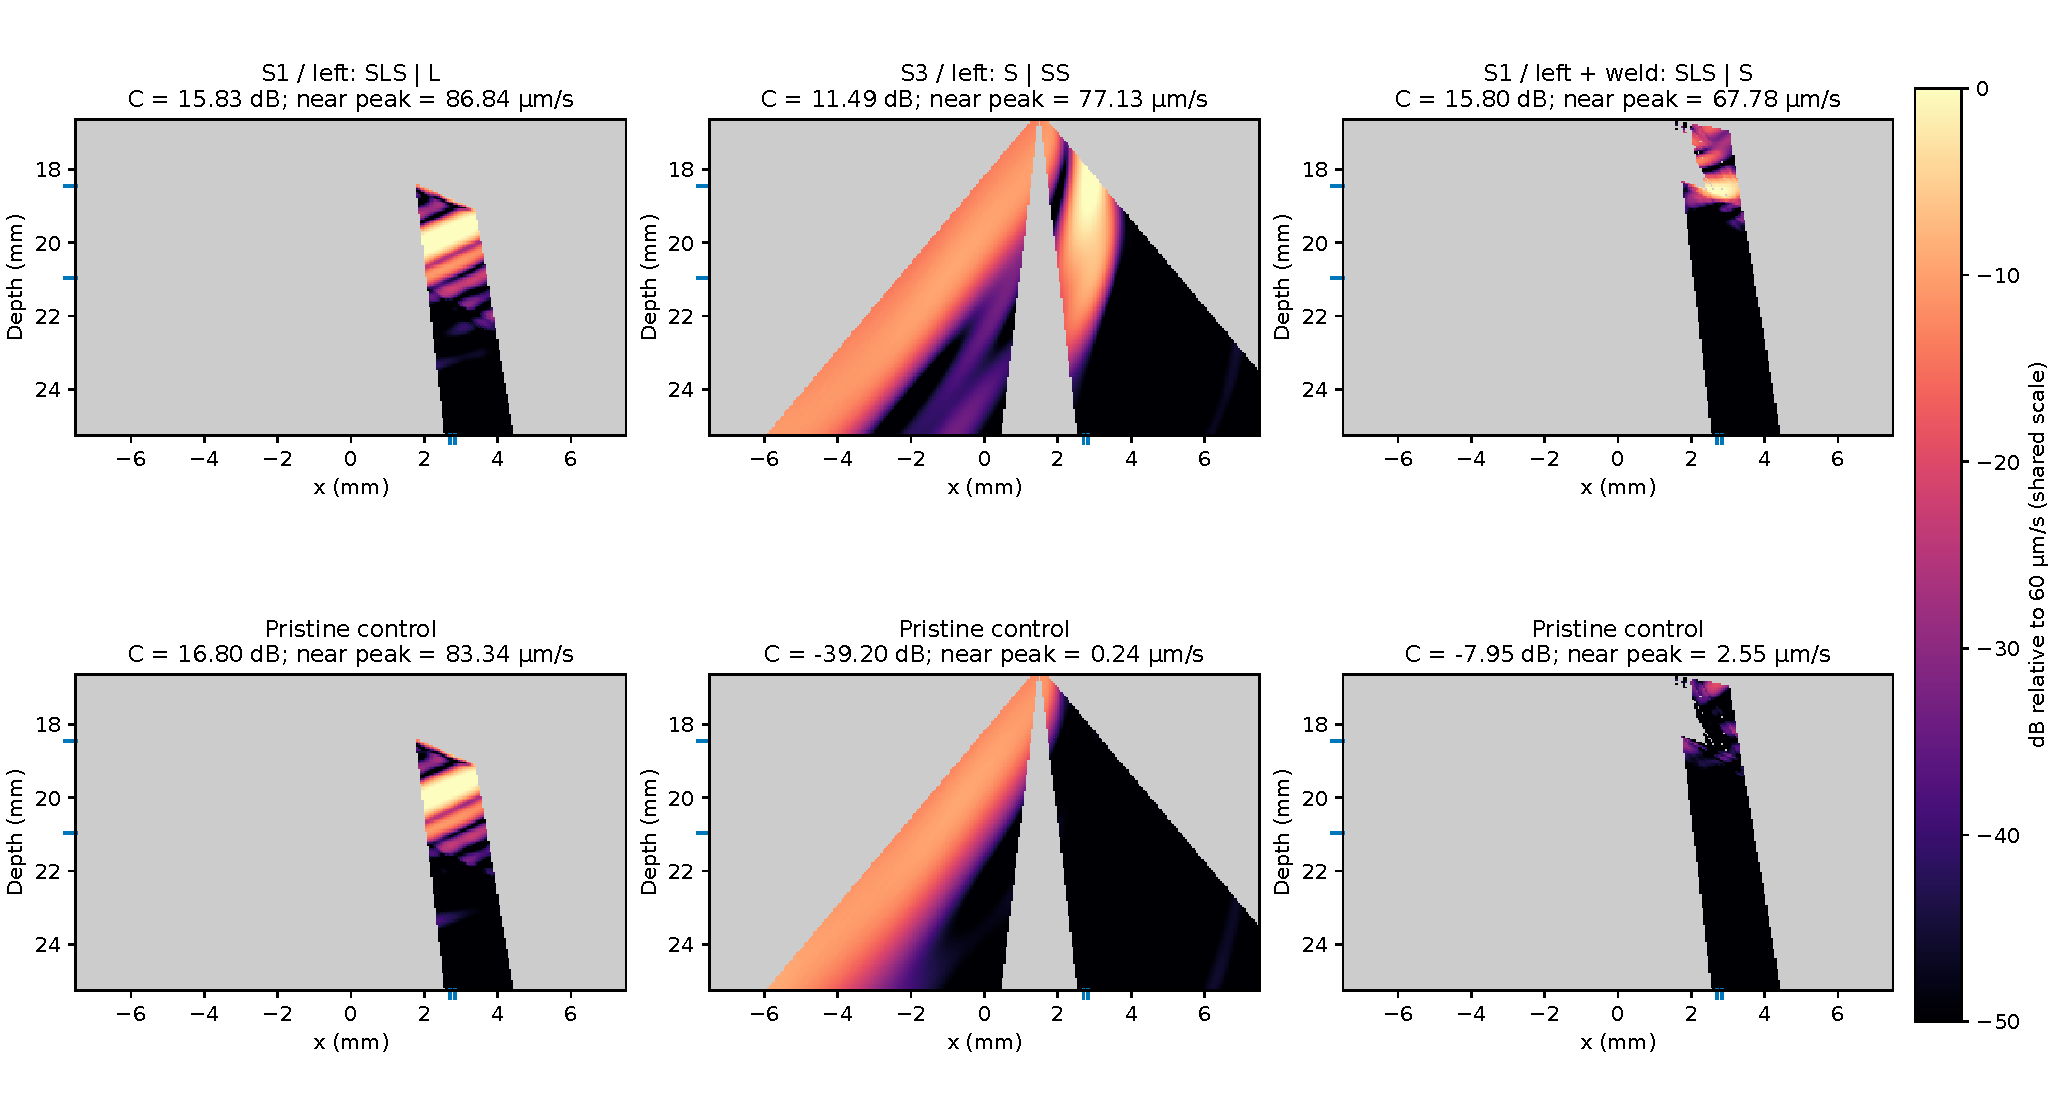
\includegraphics[width=\linewidth]{figures/saft_appendix/review/atlas_controls.pdf}
\caption{Three follow-up examples at 0.05 mm: a high-scoring pristine lookalike ($SLS\mid L$, S1/left), a useful single-shot shear view ($S\mid SS$, S3/left), and a broader complementary path ($SLS\mid S$, S1/left+weld). LOF-only and pristine controls share one absolute scale. The complete follow-up table also reports wider-field failures.}
\label{saftapp:atlas_controls}
\end{figure}

The group recombination is checked against 16 independently requested native reconstructions (48 signal cases). The complete atlas also checks every original single-group image against its reconstructed statistics. The source-subset follow-up evaluates all 31 nonempty fixed subsets and every feasible source-count minimum, giving 80 views per signal case on the 0.05 mm candidate grid. A reduced set can retain a high near-flaw score while losing much of the total assessed field. The all-five-source candidate remains the principal working choice; the source-subset register exposes this coverage cost.

\subsection{Settings matrix and interpretation}
The 252 native settings configurations comprise 63 variants on four anchors: all-source/all-receiver $S\mid SS$; three weld sources with left receivers for $S\mid SS$; S3 with right receivers for $S\mid LL$; and S1 with right receivers for $SSL\mid SS$. The latter two require one source because only one shot is selected. Table~\ref{saftapp:control_inventory} states the controls covered. These are representative one-factor sensitivities plus all reflected-screen combinations, not every possible Cartesian combination of continuous settings or arbitrary receiver masks.

\begin{longtable}{@{}>{\raggedright\arraybackslash}p{.27\linewidth}>{\raggedright\arraybackslash}p{.67\linewidth}@{}}
\caption{Controls examined in the partial-weld review. Baseline values are included where not repeated in the variation list.}\label{saftapp:control_inventory}\\
\toprule Control & Values and purpose\\\midrule\endfirsthead
\toprule Control & Values and purpose\\\midrule\endhead
Frequency band & 0.5--3, 0.5--5, 1--3, 1--5, 1.5--5 and 2--5 MHz; historical fourteen-filter comparison retained separately.\\
Angular gate & 0, 5, 10, 15, 20 and 30\% launch/reception magnitudes.\\
Wall gate / exclusion & Wall response 0, 2.5, 5 and 10\%; source--receiver exclusion 0, 0.75, 1.5, 3 and 5 mm.\\
Response / component & Equal or complex response-weighted mean; normal $v_y$, with tangential $v_x$ as a diagnostic outside the assumed normal optical measurement.\\
Direct screens & All eight combinations of L, S and Rayleigh; tail levels 20, 30, 40 dB and margins 0, 0.05, 0.1, 0.2 $\mu$s.\\
Reflected screens & All 16 combinations of LL, LS/SL, SS and repeated SSSS packet screening.\\
Fixed arrival mutes & Each of R, L, S, LL, LS/SL and SS separately, and all together. Width checks include 0.1--0.8 and 1.2 $\mu$s.\\
Physical / relative aperture & All seven combinations of left, weld and right surfaces; receiver subsets relative to the trial pixel (left/right); interleaved even/odd receiver IDs.\\
Source choices & Five individual shots, weld and all-shot views; all 31 fixed subsets with every feasible source-count minimum for the candidate.\\
Retention guards & Fraction 0, 0.1, 0.25, 0.5, 1; actual floors 1, 4, 8, 16, 32; effective floors 0, 4, 8, 16, 32; relaxed guards and source-count/fixed-source policies.\\
Coherence / combination & CF powers 0, 0.5, 1, 2; RMS versus coherent source averaging. These alter the score, not the acquired acoustic information.\\
Record repairs / frozen aperture & Case-local and paired repair rejection; an aperture frozen at $(0,20)$ mm, independent of the flaw coordinates. Paired repair metadata are a reference-assisted diagnostic.\\
Image grid / field & 0.2, 0.1, 0.05, 0.025 mm; half-pixel shift at 0.05 mm; wider $x=\pm45$ mm fields. Display reference and clipping never enter numerical metrics.\\
\bottomrule
\end{longtable}

The full settings matrix below reports each native variation, including failures. Offline qualification and coherence variations reuse sufficient statistics; they are distinct from new propagation or filtering calculations. The evidence bundle retains their complete metrics, selections and checks. Thread count and colour-display controls do not define a different physical reconstruction and are not treated as tuning variables.

\begingroup\small\setlength{\tabcolsep}{3pt}
\begin{longtable}{@{}lrrrr@{}}
\caption{Complete native settings matrix at 0.2 mm: each cell is contrast in dB / near support in percent. Dashes indicate undefined contrast. Labels follow the reproducible protocol; mute0--5 correspond to R, L, S, LL, LS/SL and SS. Reflected bit strings use the stored order (least significant first): LL, LS/SL, SS, SSSS.}\label{saftapp:settings_matrix}\\
\toprule Variant & All $S\mid SS$ & Left $S\mid SS$ & S3 $S\mid LL$ & S1 $SSL\mid SS$\\\midrule\endfirsthead
\toprule Variant & All $S\mid SS$ & Left $S\mid SS$ & S3 $S\mid LL$ & S1 $SSL\mid SS$\\\midrule\endhead
baseline & 8.72 / 95 & 10.72 / 54 & 3.03 / 95 & 3.15 / 100\\
band0.5\_\allowbreak 3 & 1.46 / 100 & 0.01 / 81 & -1.78 / 96 & -1.22 / 93\\
band0.5\_\allowbreak 5 & 8.46 / 95 & 7.78 / 54 & 2.47 / 95 & 3.45 / 100\\
band1\_\allowbreak 3 & 1.77 / 100 & 3.72 / 77 & -1.37 / 96 & -1.16 / 95\\
band1.5\_\allowbreak 5 & 8.72 / 95 & 11.68 / 54 & 1.16 / 95 & 8.95 / 100\\
band2\_\allowbreak 5 & 8.44 / 95 & 10.17 / 53 & -3.52 / 95 & 4.48 / 100\\
angular0 & 2.13 / 100 & 5.14 / 100 & 1.35 / 100 & 0.79 / 100\\
angular0.05 & 2.13 / 100 & 5.07 / 100 & 1.35 / 99 & 0.79 / 100\\
angular0.1 & 0.86 / 100 & 5.05 / 98 & 1.35 / 99 & 1.10 / 100\\
angular0.2 & 8.80 / 95 & 10.13 / 51 & 3.03 / 95 & 8.04 / 75\\
angular0.3 & 8.64 / 93 & 9.67 / 22 & 5.76 / 69 & -- / 0\\
wall0 & 8.72 / 95 & 10.72 / 54 & 3.03 / 95 & 3.34 / 100\\
wall0.025 & 8.72 / 95 & 10.72 / 54 & 3.03 / 95 & 3.34 / 100\\
wall0.1 & 8.72 / 95 & 10.72 / 54 & 3.03 / 95 & 3.20 / 100\\
offset0 & 8.66 / 95 & 10.72 / 54 & 3.03 / 95 & 3.15 / 100\\
offset0.75 & 8.67 / 95 & 10.72 / 54 & 3.03 / 95 & 3.15 / 100\\
offset3 & 8.83 / 95 & 10.72 / 54 & 3.03 / 95 & 3.15 / 100\\
offset5 & 8.87 / 95 & 10.72 / 54 & 3.03 / 95 & 3.15 / 100\\
equal & 4.45 / 95 & 11.93 / 54 & -0.54 / 95 & -10.47 / 100\\
tangential & -0.98 / 95 & -8.62 / 54 & -8.59 / 95 & -23.91 / 100\\
screen\_\allowbreak off & 8.72 / 95 & 10.72 / 54 & 3.03 / 95 & 3.15 / 100\\
screen\_\allowbreak L & 8.72 / 95 & 10.72 / 54 & 3.03 / 95 & 3.15 / 100\\
screen\_\allowbreak S & 8.72 / 95 & 10.72 / 54 & 3.03 / 95 & 3.15 / 100\\
screen\_\allowbreak R & 8.72 / 95 & 10.72 / 54 & 3.03 / 95 & 3.15 / 100\\
screen\_\allowbreak LS & 8.72 / 95 & 10.72 / 54 & 3.03 / 95 & 3.15 / 100\\
screen\_\allowbreak LR & 8.72 / 95 & 10.72 / 54 & 3.03 / 95 & 3.15 / 100\\
screen\_\allowbreak SR & 8.72 / 95 & 10.72 / 54 & 3.03 / 95 & 3.15 / 100\\
reflect0001 & 8.83 / 95 & 10.72 / 54 & -- / 0 & 3.15 / 100\\
reflect0010 & -- / 0 & 0.72 / 5 & -- / 0 & 3.15 / 100\\
reflect0011 & -- / 0 & 0.72 / 5 & -- / 0 & 3.15 / 100\\
reflect0100 & -- / 0 & -- / 0 & 3.03 / 95 & 3.15 / 100\\
reflect0101 & -- / 0 & -- / 0 & -- / 0 & 3.15 / 100\\
reflect0110 & -- / 0 & -- / 0 & -- / 0 & 3.15 / 100\\
reflect0111 & -- / 0 & -- / 0 & -- / 0 & 3.15 / 100\\
reflect1000 & 8.72 / 95 & 10.72 / 54 & 3.03 / 95 & 3.30 / 100\\
reflect1001 & 8.83 / 95 & 10.72 / 54 & -- / 0 & 3.30 / 100\\
reflect1010 & -- / 0 & 0.72 / 5 & -- / 0 & 3.30 / 100\\
reflect1011 & -- / 0 & 0.72 / 5 & -- / 0 & 3.30 / 100\\
reflect1100 & -- / 0 & -- / 0 & 3.03 / 95 & 3.30 / 100\\
reflect1101 & -- / 0 & -- / 0 & -- / 0 & 3.30 / 100\\
reflect1110 & -- / 0 & -- / 0 & -- / 0 & 3.30 / 100\\
reflect1111 & -- / 0 & -- / 0 & -- / 0 & 3.30 / 100\\
tail20 & 8.72 / 95 & 10.72 / 54 & 3.03 / 95 & 3.15 / 100\\
tail40 & 8.72 / 95 & 10.72 / 54 & 3.03 / 95 & 3.15 / 100\\
margin0 & 8.72 / 95 & 10.72 / 54 & 3.03 / 95 & 3.15 / 100\\
margin0.05 & 8.72 / 95 & 10.72 / 54 & 3.03 / 95 & 3.15 / 100\\
margin0.2 & 8.72 / 95 & 10.72 / 54 & 3.03 / 95 & 3.15 / 100\\
mute0 & 8.72 / 95 & 10.72 / 54 & 3.03 / 95 & 3.15 / 100\\
mute1 & 8.72 / 95 & 10.72 / 54 & 3.03 / 95 & 3.15 / 100\\
mute2 & 8.72 / 95 & 10.72 / 54 & 3.03 / 95 & 3.15 / 100\\
mute3 & 8.72 / 95 & 10.72 / 54 & -11.64 / 70 & 3.15 / 100\\
mute4 & 8.72 / 95 & 10.72 / 54 & 3.03 / 95 & 3.15 / 100\\
mute5 & 15.28 / 88 & 12.48 / 54 & 3.03 / 95 & 3.15 / 100\\
mute\_\allowbreak all & 15.28 / 88 & 12.48 / 54 & -1.99 / 70 & 3.15 / 100\\
mute\_\allowbreak all\_\allowbreak width0.3 & 15.77 / 95 & 10.67 / 54 & 7.94 / 95 & 3.15 / 100\\
mute\_\allowbreak all\_\allowbreak width1.2 & 7.41 / 51 & 2.53 / 12 & -- / 0 & 3.15 / 100\\
aperture\_\allowbreak left & 10.04 / 95 & 10.72 / 54 & -- / 0 & -- / 0\\
aperture\_\allowbreak right & -3.24 / 95 & -- / 0 & 3.03 / 95 & 3.15 / 100\\
aperture\_\allowbreak even & 8.78 / 95 & 10.66 / 54 & 2.84 / 95 & 5.70 / 100\\
aperture\_\allowbreak odd & 8.65 / 95 & 10.70 / 54 & 3.32 / 95 & 4.72 / 100\\
clean\_\allowbreak case & 8.72 / 95 & 10.72 / 54 & 3.03 / 95 & 3.15 / 100\\
clean\_\allowbreak paired & 8.72 / 95 & 10.72 / 54 & 3.03 / 95 & 3.15 / 100\\
frozen\_\allowbreak centre & 3.93 / 5 & 0.66 / 5 & 3.40 / 95 & -- / 0\\
\bottomrule\end{longtable}\endgroup

The 25\% retention threshold is an engineering guard, not a literature-derived detection criterion. In the original all-aperture anchors it is inactive, even when raised to 100\% of the already eligible receivers. In contrast, broad reflected-pulse exclusion can make retention or time support restrictive. It is therefore incorrect either to blame the 25\% rule for the original missing region or to assume it is irrelevant for every new path and screen. The receiver-fraction audit, source-count audit and angular audit answer different questions.

\subsection{Why a short arrival mute helps, and what it does not prove}
The fixed mute suppresses samples near a predicted specimen-only backwall arrival that could otherwise be focused under a flaw-scattering delay. It is applied to every trial pixel by its predicted time, without a flaw-location window. The result nevertheless depends on a width selected using the known example. Its improvement can involve less destructive cancellation and higher receiver coherence as well as reduced nuisance contributions. Accordingly, a larger output peak is not interpreted as greater measured energy or calibrated signal-to-noise ratio.

\begin{figure}[!htbp]\centering
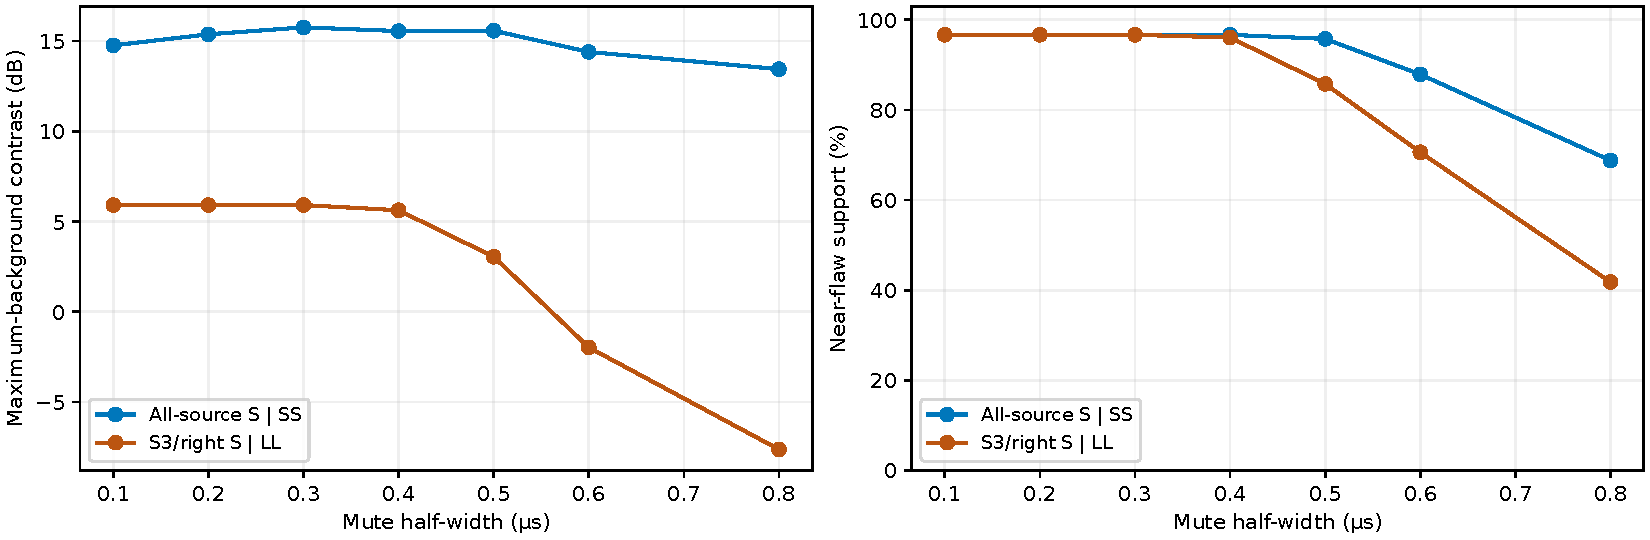
\includegraphics[width=\linewidth]{figures/saft_appendix/review/mute_sensitivity.pdf}
\caption{Fixed-mute width sensitivity at 0.1 mm. These sweeps activate all six predicted-arrival mute families; their narrower 0.3 $\mu$s result is then simplified to SS-only for $S\mid SS$ and LL-only for the single-shot $S\mid LL$ view. The independent family checks and finer/wider images test that simplification. Support drops as the excluded interval expands. A smooth curve between sampled widths is not assumed.}
\label{saftapp:mute_sensitivity}
\end{figure}

For all-source $S\mid SS$, widths 0.1--0.5 $\mu$s give about 14.8--15.8 dB on the 0.1 mm grid. Width 0.6 $\mu$s reduces near support to 87.9\%, and 0.8 $\mu$s to 68.8\%. The 0.3 $\mu$s choice therefore lies in a useful tested range rather than at a single isolated sharp optimum. Even/odd receiver subsets retain 15.65/15.78 dB with 96.7\% near support. The narrower single-shot $S\mid LL$ view is more sensitive: widths 0.1--0.3 $\mu$s give 5.92 dB, while 0.6 $\mu$s gives $-1.97$ dB and only 70.6\% support.

Increasing the coherence exponent to two also raises local contrast, but the updated principal recipe retains exponent one. A more nonlinear display score is not additional evidence of independent scattering. Similarly, increasing the lower frequency cutoff can improve local $SSL\mid SS$ contrast while leaving a dominant remote false indication. These controls are useful precisely because they prevent every numerical contrast gain from being called an imaging improvement.

\subsection{Single weld shots and right-side receivers}
The 157 right receivers span approximately $x=4.5534$--43.5534 mm. For S3 and $S\mid LL$, the retained signal is much stronger in absolute amplitude than the multi-bounce S1 $SSL\mid SS$ candidate. The earlier right-side survey includes all 132 conventional sequences and 20 short sequences on near (below 15 mm), middle (15--35 mm) and far (above 35 mm) right-receiver windows. All controls use the declared fixed window throughout the image.

\begin{figure}[!htbp]\centering
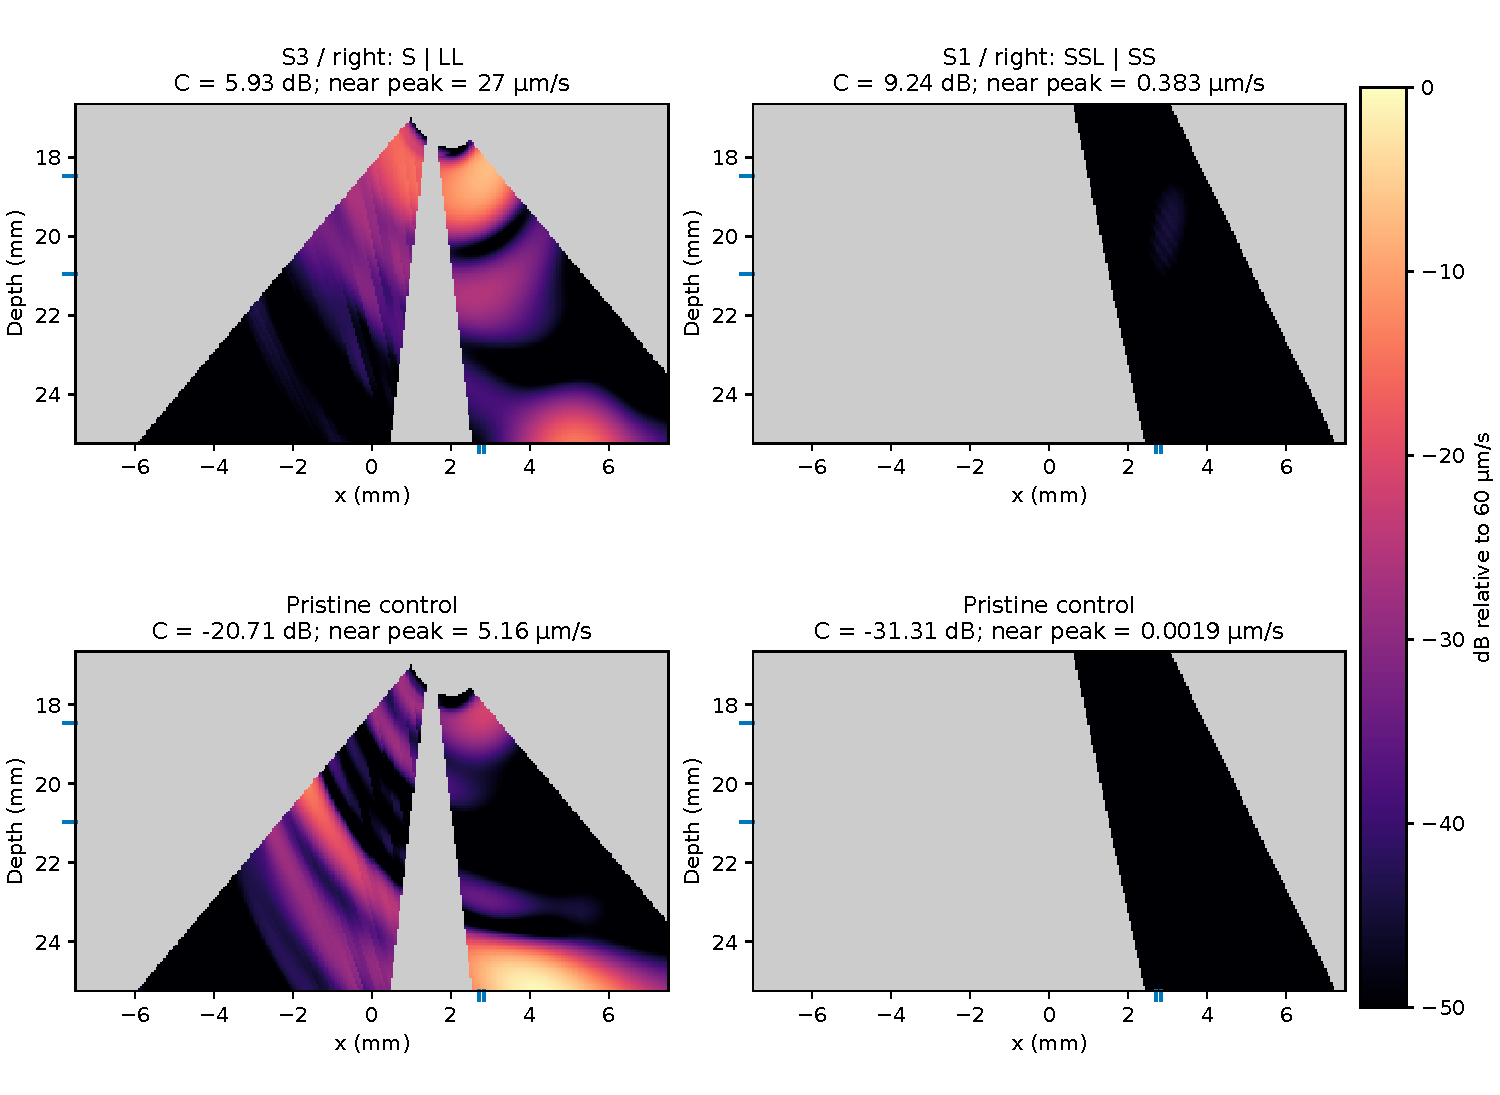
\includegraphics[width=\linewidth]{figures/saft_appendix/review/right_paths_controls.pdf}
\caption{Two fixed weld-source/right-receiver alternatives. The useful S3 $S\mid LL$ view uses 1--5 MHz and the narrow LL mute. S1 $SSL\mid SS$ uses 1.5--5 MHz without a fixed mute. LOF and pristine panels use the same absolute scale, making their very different amplitudes visible. Both are at 0.05 mm. Neither delay label uniquely identifies a physical packet in the mixed recordings.}
\label{saftapp:right_controls}
\end{figure}
\begin{figure}[!htbp]\centering
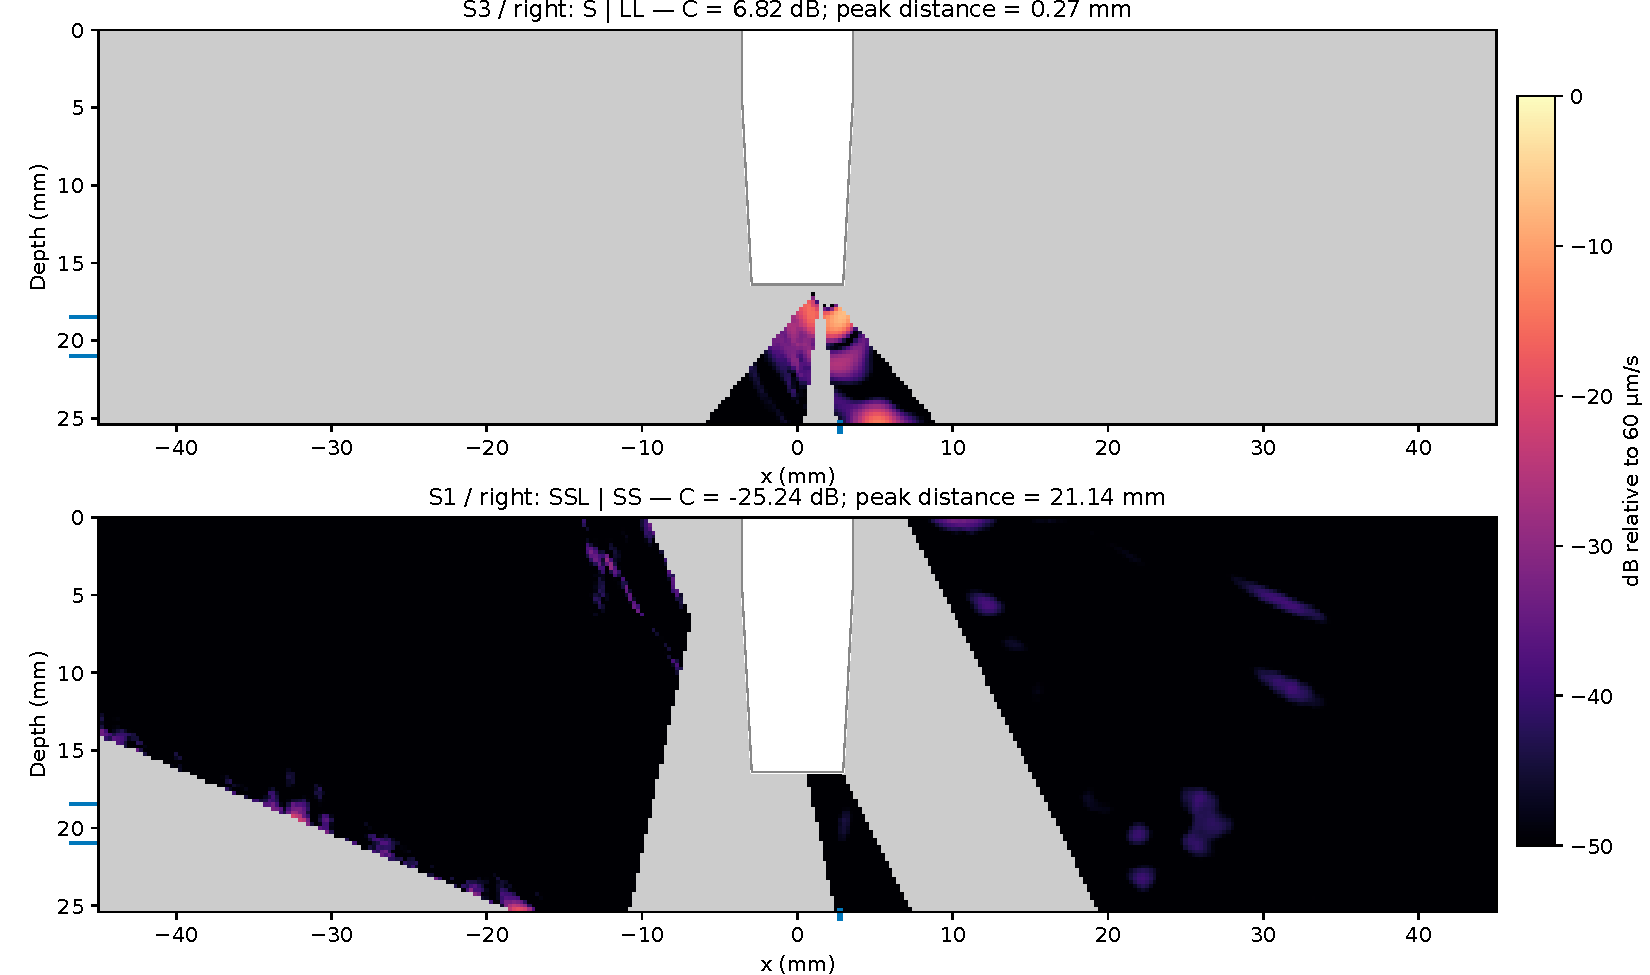
\includegraphics[width=\linewidth]{figures/saft_appendix/review/right_paths_wide.pdf}
\caption{The same alternatives on the wider field at 0.25 mm. The $S\mid LL$ indication survives with 6.82 dB contrast; the apparently improved local $SSL\mid SS$ image fails with $-25.24$ dB. Common absolute scaling is retained, rather than independently brightening the weaker route.}
\label{saftapp:right_wide}
\end{figure}

The $S\mid LL$ near response is not cleanly separable from every predicted reflected packet. Activating the full measured reflected-pulse screens removes its near support. The short LL mute retains information by excluding less time, but cannot by itself prove an isolated flaw-converted wave. The correct conclusion is that this fixed acquisition contains useful defect-associated focusing information, supported by pristine/difference controls and a wider field. It is a candidate supplementary acquisition, not a demonstrated mode-pure detection channel.

\subsection{Grid, source coverage and remaining uncertainty}
The finest matched mute comparison uses 207,345 image pixels at 0.025 mm. The shifted 0.05 mm comparison gives 14.45 dB muted and 9.07 dB unmuted, consistent with the finer-grid conclusions. The change from 15.77 dB on the original 0.05 mm grid illustrates the sensitivity of a maximum-background statistic to narrow peaks and changing apertures. These checks do not claim complete asymptotic grid convergence. Wider-field sampling is stated separately, and it is not evidence of finite-element mesh convergence.

The principal two-source recipe supports only 3.76\% of the entire 90 mm by 25 mm wider field at 0.1 mm. Its wider-field contrast therefore concerns assessed pixels, not verified inspection coverage across the plate. This is compatible with high support around the prescribed flaw and must not be hidden by cropping grey areas.

The known defect coordinates enter retrospective metrics and external figure guides, not travel-time calculation, channel gates, the frozen-aperture anchor or the fixed-mute centres. Nonetheless, selecting among many configurations using one known flaw introduces selection bias. Independent flaw locations, dimensions, noise, material variation and model convergence are still needed before choosing a robust instrument prescription. No probability of detection, reliable flaw sizing or experimental energy sensitivity follows from the current contrasts.

\subsection{Complete path and source registers}
The following compact path register gives the best observed fixed view per path among views with at least 20\% near support. It is an exploratory summary, not a proposed per-pixel combination or a claim of optimal acquisition. A dash means no view meets that coverage floor. The machine-readable atlas retains all views, all three signal cases, amplitudes, support, pristine ratio and peak locations. Corner timing models retain uncalibrated corner amplitude and phase.

\begingroup\small\setlength{\tabcolsep}{3pt}
\begin{longtable}{@{}r>{\raggedright\arraybackslash}p{.28\linewidth}>{\raggedright\arraybackslash}p{.27\linewidth}rrr@{}}
\caption{All 324 path hypotheses, ordered as in the native catalogue. Best fixed view with at least 20\% near support: $C$ in dB, N in percent and peak distance in mm. This retrospective ranking is not a per-pixel fusion rule. Exact identifiers and all unselected views are retained in atlas\_metrics.csv.}\label{saftapp:path_register}\\
\toprule No. & Path identifier & Receiver group / source view & $C$ & N & $d_{\rm pk}$\\\midrule\endfirsthead
\toprule No. & Path identifier & Receiver group / source view & $C$ & N & $d_{\rm pk}$\\\midrule\endhead
1 & $L\mid L$ & right / source2 & -5.54 & 100 & 1.65\\
2 & $L\mid S$ & sides / weld\_\allowbreak min1 & -13.27 & 100 & 1.84\\
3 & $S\mid L$ & all / all\_\allowbreak min2 & -11.60 & 95 & 4.32\\
4 & $S\mid S$ & sides / source4 & -5.46 & 100 & 4.45\\
5 & $LL\mid L$ & right / source0 & -4.43 & 100 & 4.40\\
6 & $LL\mid S$ & left / source4 & -5.94 & 72 & 3.04\\
7 & $LS\mid L$ & left / weld\_\allowbreak min1 & 4.39 & 75 & 0.11\\
8 & $LS\mid S$ & left\_\allowbreak weld / source1 & -0.93 & 99 & 0.91\\
9 & $SL\mid L$ & weld / source4 & -0.17 & 100 & 2.36\\
10 & $SL\mid S$ & left / source1 & 14.18 & 75 & 0.52\\
11 & $SS\mid L$ & weld / weld\_\allowbreak min1 & -6.09 & 100 & 1.12\\
12 & $SS\mid S$ & left\_\allowbreak weld / source1 & 7.45 & 99 & 0.33\\
13 & $L\mid LL$ & right / source3 & -0.10 & 72 & 1.07\\
14 & $L\mid LS$ & weld / all\_\allowbreak min1 & 1.47 & 99 & 0.33\\
15 & $L\mid SL$ & left / source4 & -1.76 & 100 & 4.95\\
16 & $L\mid SS$ & all / source4 & 3.73 & 100 & 0.29\\
17 & $S\mid LL$ & weld\_\allowbreak right / source3 & 3.42 & 95 & 0.23\\
18 & $S\mid LS$ & sides / source4 & -3.21 & 100 & 4.30\\
19 & $S\mid SL$ & sides / source4 & 0.57 & 100 & 0.09\\
20 & $S\mid SS$ & left / source2 & 12.92 & 54 & 0.07\\
21 & $LL\mid LL$ & weld / source4 & -0.81 & 83 & 4.29\\
22 & $LL\mid LS$ & weld / source4 & 6.55 & 82 & 0.44\\
23 & $LL\mid SL$ & weld / weld\_\allowbreak min1 & -1.83 & 51 & 3.03\\
24 & $LL\mid SS$ & weld / source4 & 1.79 & 83 & 0.15\\
25 & $LS\mid LL$ & weld / source1 & -1.43 & 100 & 9.20\\
26 & $LS\mid LS$ & weld\_\allowbreak right / source0 & 6.53 & 100 & 0.31\\
27 & $LS\mid SL$ & sides / source4 & 16.46 & 100 & 0.10\\
28 & $LS\mid SS$ & all / source4 & 1.51 & 100 & 0.51\\
29 & $SL\mid LL$ & weld / source1 & -1.14 & 100 & 8.18\\
30 & $SL\mid LS$ & weld / source4 & 2.59 & 99 & 0.62\\
31 & $SL\mid SL$ & weld / weld\_\allowbreak min1 & -1.22 & 64 & 6.30\\
32 & $SL\mid SS$ & sides / source4 & 7.80 & 100 & 0.48\\
33 & $SS\mid LL$ & weld / source1 & -3.16 & 100 & 8.00\\
34 & $SS\mid LS$ & weld / source4 & -6.66 & 99 & 1.42\\
35 & $SS\mid SL$ & weld / weld\_\allowbreak min1 & -2.38 & 67 & 5.71\\
36 & $SS\mid SS$ & sides / source4 & 2.34 & 100 & 0.41\\
37 & $L\mid LLL$ & all / source2 & 4.02 & 100 & 0.48\\
38 & $L\mid LLS$ & left\_\allowbreak weld / source4 & -5.61 & 100 & 4.73\\
39 & $L\mid LSL$ & weld / source3 & 0.28 & 72 & 0.05\\
40 & $L\mid LSS$ & weld / source3 & 0.63 & 55 & 0.11\\
41 & $L\mid SLL$ & weld / weld\_\allowbreak min2 & 4.53 & 34 & 0.10\\
42 & $L\mid SLS$ & sides / source2 & -22.19 & 100 & 3.80\\
43 & $L\mid SSL$ & weld / weld\_\allowbreak min2 & 0.77 & 41 & 0.10\\
44 & $L\mid SSS$ & weld / source4 & 2.88 & 82 & 0.49\\
45 & $S\mid LLL$ & left\_\allowbreak weld / all\_\allowbreak min2 & 3.29 & 95 & 0.28\\
46 & $S\mid LLS$ & sides / weld\_\allowbreak min2 & -26.48 & 54 & 5.12\\
47 & $S\mid LSL$ & weld / source3 & 5.15 & 75 & 0.11\\
48 & $S\mid LSS$ & weld / source3 & 4.44 & 51 & 0.53\\
49 & $S\mid SLL$ & weld / source3 & 0.84 & 92 & 0.23\\
50 & $S\mid SLS$ & all / all\_\allowbreak min2 & -11.50 & 95 & 4.32\\
51 & $S\mid SSL$ & weld / source3 & -0.48 & 92 & 2.13\\
52 & $S\mid SSS$ & weld / source4 & 9.32 & 82 & 0.53\\
53 & $LLL\mid L$ & left / all\_\allowbreak min1 & -11.08 & 75 & 3.48\\
54 & $LLL\mid S$ & left / source0 & 0.11 & 75 & 0.52\\
55 & $LLS\mid L$ & left / source0 & -16.53 & 75 & 3.48\\
56 & $LLS\mid S$ & left / source0 & 1.54 & 75 & 0.52\\
57 & $LSL\mid L$ & left / source0 & 19.16 & 75 & 0.52\\
58 & $LSL\mid S$ & left\_\allowbreak weld / all\_\allowbreak min1 & 5.41 & 100 & 0.49\\
59 & $LSS\mid L$ & left\_\allowbreak weld / source1 & 20.30 & 36 & 0.13\\
60 & $LSS\mid S$ & weld / source1 & 16.17 & 30 & 0.08\\
61 & $SLL\mid L$ & left\_\allowbreak weld / source1 & 0.42 & 89 & 0.99\\
62 & $SLL\mid S$ & weld / source1 & 15.58 & 57 & 0.50\\
63 & $SLS\mid L$ & left / source1 & 31.76 & 75 & 0.26\\
64 & $SLS\mid S$ & left / source1 & 23.25 & 75 & 0.11\\
65 & $SSL\mid L$ & left / weld\_\allowbreak min2 & 3.83 & 20 & 0.91\\
66 & $SSL\mid S$ & left\_\allowbreak weld / source2 & 11.67 & 23 & 0.10\\
67 & $SSS\mid L$ & left / weld\_\allowbreak min2 & 18.61 & 52 & 0.11\\
68 & $SSS\mid S$ & left\_\allowbreak weld / source2 & 5.57 & 54 & 0.09\\
69 & $LL\mid LLL$ & left / source4 & -4.65 & 83 & 4.32\\
70 & $LL\mid LLS$ & left / source4 & -3.63 & 83 & 3.78\\
71 & $LL\mid LSL$ & weld / source4 & -0.55 & 51 & 3.92\\
72 & $LL\mid LSS$ & weld / source0 & -2.47 & 55 & 1.13\\
73 & $LL\mid SLL$ & sides / source0 & -2.56 & 100 & 1.22\\
74 & $LL\mid SLS$ & sides / source0 & 0.57 & 100 & 0.91\\
75 & $LL\mid SSL$ & weld / source1 & 5.52 & 31 & 0.28\\
76 & $LL\mid SSS$ & all / weld\_\allowbreak min1 & -8.77 & 59 & 4.35\\
77 & $LS\mid LLL$ & weld / source4 & 6.64 & 99 & 0.48\\
78 & $LS\mid LLS$ & left / source0 & -1.78 & 100 & 1.28\\
79 & $LS\mid LSL$ & weld / source0 & 6.35 & 30 & 0.38\\
80 & $LS\mid LSS$ & weld / source4 & 0.30 & 55 & 0.70\\
81 & $LS\mid SLL$ & weld / source0 & 0.92 & 94 & 0.27\\
82 & $LS\mid SLS$ & weld\_\allowbreak right / source0 & -4.76 & 100 & 1.06\\
83 & $LS\mid SSL$ & left / source4 & -0.06 & 100 & 1.54\\
84 & $LS\mid SSS$ & left / source0 & 0.42 & 100 & 0.66\\
85 & $SL\mid LLL$ & weld / source4 & -0.01 & 99 & 1.05\\
86 & $SL\mid LLS$ & right / source4 & -0.22 & 100 & 0.70\\
87 & $SL\mid LSL$ & right / source1 & -0.09 & 100 & 2.19\\
88 & $SL\mid LSS$ & weld / source0 & 0.81 & 55 & 0.32\\
89 & $SL\mid SLL$ & weld / source4 & -11.58 & 94 & 2.38\\
90 & $SL\mid SLS$ & right / weld\_\allowbreak min2 & -20.44 & 93 & 4.57\\
91 & $SL\mid SSL$ & weld / source4 & 0.76 & 95 & 0.67\\
92 & $SL\mid SSS$ & weld / source4 & 4.85 & 82 & 0.28\\
93 & $SS\mid LLL$ & weld / source4 & -7.94 & 99 & 4.57\\
94 & $SS\mid LLS$ & right / source4 & -23.96 & 100 & 4.32\\
95 & $SS\mid LSL$ & weld / all\_\allowbreak min1 & -8.42 & 33 & 8.38\\
96 & $SS\mid LSS$ & weld / source0 & -2.66 & 55 & 6.48\\
97 & $SS\mid SLL$ & sides / source4 & 1.26 & 100 & 0.63\\
98 & $SS\mid SLS$ & right / source1 & -3.46 & 100 & 9.29\\
99 & $SS\mid SSL$ & left / source0 & -2.62 & 100 & 1.44\\
100 & $SS\mid SSS$ & sides / source4 & -0.86 & 100 & 1.88\\
101 & $LLL\mid LL$ & left\_\allowbreak weld / source0 & 2.62 & 100 & 0.91\\
102 & $LLL\mid LS$ & all / source0 & 4.16 & 100 & 0.89\\
103 & $LLL\mid SL$ & left / source0 & -13.87 & 100 & 3.53\\
104 & $LLL\mid SS$ & left\_\allowbreak weld / source0 & -3.11 & 100 & 5.47\\
105 & $LLS\mid LL$ & left\_\allowbreak weld / source0 & -3.95 & 100 & 1.25\\
106 & $LLS\mid LS$ & left\_\allowbreak weld / source0 & 0.01 & 100 & 0.86\\
107 & $LLS\mid SL$ & weld / source0 & -5.87 & 100 & 3.62\\
108 & $LLS\mid SS$ & weld / source0 & -2.71 & 100 & 4.73\\
109 & $LSL\mid LL$ & weld / all\_\allowbreak min1 & -2.89 & 100 & 5.66\\
110 & $LSL\mid LS$ & weld / source0 & -1.06 & 99 & 1.69\\
111 & $LSL\mid SL$ & left / source0 & -2.77 & 100 & 3.28\\
112 & $LSL\mid SS$ & weld / all\_\allowbreak min1 & -8.18 & 100 & 4.74\\
113 & $LSS\mid LL$ & left\_\allowbreak weld / source1 & 21.37 & 36 & 0.49\\
114 & $LSS\mid LS$ & all / source1 & 11.45 & 36 & 0.08\\
115 & $LSS\mid SL$ & right / source1 & -0.42 & 36 & 1.85\\
116 & $LSS\mid SS$ & sides / source1 & 1.96 & 36 & 0.67\\
117 & $SLL\mid LL$ & weld\_\allowbreak right / source1 & 0.63 & 89 & 0.21\\
118 & $SLL\mid LS$ & all / source1 & 0.34 & 89 & 0.70\\
119 & $SLL\mid SL$ & weld / source1 & -6.50 & 25 & 4.16\\
120 & $SLL\mid SS$ & left\_\allowbreak weld / source0 & 0.92 & 100 & 0.23\\
121 & $SLS\mid LL$ & all / source1 & -7.56 & 99 & 4.28\\
122 & $SLS\mid LS$ & sides / source1 & 5.36 & 99 & 0.08\\
123 & $SLS\mid SL$ & left / source0 & 2.00 & 100 & 0.51\\
124 & $SLS\mid SS$ & all / source1 & 2.08 & 99 & 0.29\\
125 & $SSL\mid LL$ & weld\_\allowbreak right / weld\_\allowbreak min2 & -0.08 & 42 & 0.53\\
126 & $SSL\mid LS$ & weld / source0 & 2.28 & 99 & 0.33\\
127 & $SSL\mid SL$ & weld / source1 & 2.00 & 46 & 0.14\\
128 & $SSL\mid SS$ & weld\_\allowbreak right / weld\_\allowbreak min2 & 8.59 & 42 & 0.11\\
129 & $SSS\mid LL$ & weld / source1 & -1.98 & 100 & 1.91\\
130 & $SSS\mid LS$ & weld / source0 & 2.86 & 99 & 0.63\\
131 & $SSS\mid SL$ & all / weld\_\allowbreak min1 & 2.37 & 100 & 0.26\\
132 & $SSS\mid SS$ & weld / all\_\allowbreak min1 & 1.85 & 100 & 0.33\\
133 & \texttt{exp\_\allowbreak corner\_\allowbreak 1\_\allowbreak S\_\allowbreak tx\_\allowbreak direct\_\allowbreak 1} & -- & -- & -- & --\\
134 & \texttt{exp\_\allowbreak corner\_\allowbreak 1\_\allowbreak S\_\allowbreak tx\_\allowbreak direct\_\allowbreak 2} & -- & -- & -- & --\\
135 & \texttt{exp\_\allowbreak corner\_\allowbreak 1\_\allowbreak S\_\allowbreak tx\_\allowbreak id\_\allowbreak 1} & -- & -- & -- & --\\
136 & \texttt{exp\_\allowbreak corner\_\allowbreak 1\_\allowbreak S\_\allowbreak tx\_\allowbreak id\_\allowbreak 2} & -- & -- & -- & --\\
137 & \texttt{exp\_\allowbreak corner\_\allowbreak 1\_\allowbreak S\_\allowbreak tx\_\allowbreak pixel-id\_\allowbreak 1} & -- & -- & -- & --\\
138 & \texttt{exp\_\allowbreak corner\_\allowbreak 1\_\allowbreak S\_\allowbreak tx\_\allowbreak pixel-id\_\allowbreak 2} & -- & -- & -- & --\\
139 & \texttt{exp\_\allowbreak corner\_\allowbreak 1\_\allowbreak S\_\allowbreak rx\_\allowbreak direct\_\allowbreak 1} & -- & -- & -- & --\\
140 & \texttt{exp\_\allowbreak corner\_\allowbreak 1\_\allowbreak S\_\allowbreak rx\_\allowbreak direct\_\allowbreak 2} & -- & -- & -- & --\\
141 & \texttt{exp\_\allowbreak corner\_\allowbreak 1\_\allowbreak S\_\allowbreak rx\_\allowbreak id\_\allowbreak 1} & -- & -- & -- & --\\
142 & \texttt{exp\_\allowbreak corner\_\allowbreak 1\_\allowbreak S\_\allowbreak rx\_\allowbreak id\_\allowbreak 2} & -- & -- & -- & --\\
143 & \texttt{exp\_\allowbreak corner\_\allowbreak 1\_\allowbreak S\_\allowbreak rx\_\allowbreak pixel-id\_\allowbreak 1} & -- & -- & -- & --\\
144 & \texttt{exp\_\allowbreak corner\_\allowbreak 1\_\allowbreak S\_\allowbreak rx\_\allowbreak pixel-id\_\allowbreak 2} & -- & -- & -- & --\\
145 & \texttt{exp\_\allowbreak corner\_\allowbreak 1\_\allowbreak L\_\allowbreak tx\_\allowbreak direct\_\allowbreak 1} & -- & -- & -- & --\\
146 & \texttt{exp\_\allowbreak corner\_\allowbreak 1\_\allowbreak L\_\allowbreak tx\_\allowbreak direct\_\allowbreak 2} & -- & -- & -- & --\\
147 & \texttt{exp\_\allowbreak corner\_\allowbreak 1\_\allowbreak L\_\allowbreak tx\_\allowbreak id\_\allowbreak 1} & -- & -- & -- & --\\
148 & \texttt{exp\_\allowbreak corner\_\allowbreak 1\_\allowbreak L\_\allowbreak tx\_\allowbreak id\_\allowbreak 2} & -- & -- & -- & --\\
149 & \texttt{exp\_\allowbreak corner\_\allowbreak 1\_\allowbreak L\_\allowbreak tx\_\allowbreak pixel-id\_\allowbreak 1} & -- & -- & -- & --\\
150 & \texttt{exp\_\allowbreak corner\_\allowbreak 1\_\allowbreak L\_\allowbreak tx\_\allowbreak pixel-id\_\allowbreak 2} & -- & -- & -- & --\\
151 & \texttt{exp\_\allowbreak corner\_\allowbreak 1\_\allowbreak L\_\allowbreak rx\_\allowbreak direct\_\allowbreak 1} & -- & -- & -- & --\\
152 & \texttt{exp\_\allowbreak corner\_\allowbreak 1\_\allowbreak L\_\allowbreak rx\_\allowbreak direct\_\allowbreak 2} & -- & -- & -- & --\\
153 & \texttt{exp\_\allowbreak corner\_\allowbreak 1\_\allowbreak L\_\allowbreak rx\_\allowbreak id\_\allowbreak 1} & -- & -- & -- & --\\
154 & \texttt{exp\_\allowbreak corner\_\allowbreak 1\_\allowbreak L\_\allowbreak rx\_\allowbreak id\_\allowbreak 2} & -- & -- & -- & --\\
155 & \texttt{exp\_\allowbreak corner\_\allowbreak 1\_\allowbreak L\_\allowbreak rx\_\allowbreak pixel-id\_\allowbreak 1} & -- & -- & -- & --\\
156 & \texttt{exp\_\allowbreak corner\_\allowbreak 1\_\allowbreak L\_\allowbreak rx\_\allowbreak pixel-id\_\allowbreak 2} & -- & -- & -- & --\\
157 & \texttt{exp\_\allowbreak corner\_\allowbreak 2\_\allowbreak S\_\allowbreak tx\_\allowbreak direct\_\allowbreak 1} & -- & -- & -- & --\\
158 & \texttt{exp\_\allowbreak corner\_\allowbreak 2\_\allowbreak S\_\allowbreak tx\_\allowbreak direct\_\allowbreak 2} & -- & -- & -- & --\\
159 & \texttt{exp\_\allowbreak corner\_\allowbreak 2\_\allowbreak S\_\allowbreak tx\_\allowbreak id\_\allowbreak 1} & -- & -- & -- & --\\
160 & \texttt{exp\_\allowbreak corner\_\allowbreak 2\_\allowbreak S\_\allowbreak tx\_\allowbreak id\_\allowbreak 2} & -- & -- & -- & --\\
161 & \texttt{exp\_\allowbreak corner\_\allowbreak 2\_\allowbreak S\_\allowbreak tx\_\allowbreak pixel-id\_\allowbreak 1} & -- & -- & -- & --\\
162 & \texttt{exp\_\allowbreak corner\_\allowbreak 2\_\allowbreak S\_\allowbreak tx\_\allowbreak pixel-id\_\allowbreak 2} & -- & -- & -- & --\\
163 & \texttt{exp\_\allowbreak corner\_\allowbreak 2\_\allowbreak S\_\allowbreak rx\_\allowbreak direct\_\allowbreak 1} & -- & -- & -- & --\\
164 & \texttt{exp\_\allowbreak corner\_\allowbreak 2\_\allowbreak S\_\allowbreak rx\_\allowbreak direct\_\allowbreak 2} & -- & -- & -- & --\\
165 & \texttt{exp\_\allowbreak corner\_\allowbreak 2\_\allowbreak S\_\allowbreak rx\_\allowbreak id\_\allowbreak 1} & -- & -- & -- & --\\
166 & \texttt{exp\_\allowbreak corner\_\allowbreak 2\_\allowbreak S\_\allowbreak rx\_\allowbreak id\_\allowbreak 2} & -- & -- & -- & --\\
167 & \texttt{exp\_\allowbreak corner\_\allowbreak 2\_\allowbreak S\_\allowbreak rx\_\allowbreak pixel-id\_\allowbreak 1} & -- & -- & -- & --\\
168 & \texttt{exp\_\allowbreak corner\_\allowbreak 2\_\allowbreak S\_\allowbreak rx\_\allowbreak pixel-id\_\allowbreak 2} & -- & -- & -- & --\\
169 & \texttt{exp\_\allowbreak corner\_\allowbreak 2\_\allowbreak L\_\allowbreak tx\_\allowbreak direct\_\allowbreak 1} & -- & -- & -- & --\\
170 & \texttt{exp\_\allowbreak corner\_\allowbreak 2\_\allowbreak L\_\allowbreak tx\_\allowbreak direct\_\allowbreak 2} & -- & -- & -- & --\\
171 & \texttt{exp\_\allowbreak corner\_\allowbreak 2\_\allowbreak L\_\allowbreak tx\_\allowbreak id\_\allowbreak 1} & -- & -- & -- & --\\
172 & \texttt{exp\_\allowbreak corner\_\allowbreak 2\_\allowbreak L\_\allowbreak tx\_\allowbreak id\_\allowbreak 2} & -- & -- & -- & --\\
173 & \texttt{exp\_\allowbreak corner\_\allowbreak 2\_\allowbreak L\_\allowbreak tx\_\allowbreak pixel-id\_\allowbreak 1} & -- & -- & -- & --\\
174 & \texttt{exp\_\allowbreak corner\_\allowbreak 2\_\allowbreak L\_\allowbreak tx\_\allowbreak pixel-id\_\allowbreak 2} & -- & -- & -- & --\\
175 & \texttt{exp\_\allowbreak corner\_\allowbreak 2\_\allowbreak L\_\allowbreak rx\_\allowbreak direct\_\allowbreak 1} & -- & -- & -- & --\\
176 & \texttt{exp\_\allowbreak corner\_\allowbreak 2\_\allowbreak L\_\allowbreak rx\_\allowbreak direct\_\allowbreak 2} & -- & -- & -- & --\\
177 & \texttt{exp\_\allowbreak corner\_\allowbreak 2\_\allowbreak L\_\allowbreak rx\_\allowbreak id\_\allowbreak 1} & -- & -- & -- & --\\
178 & \texttt{exp\_\allowbreak corner\_\allowbreak 2\_\allowbreak L\_\allowbreak rx\_\allowbreak id\_\allowbreak 2} & -- & -- & -- & --\\
179 & \texttt{exp\_\allowbreak corner\_\allowbreak 2\_\allowbreak L\_\allowbreak rx\_\allowbreak pixel-id\_\allowbreak 1} & -- & -- & -- & --\\
180 & \texttt{exp\_\allowbreak corner\_\allowbreak 2\_\allowbreak L\_\allowbreak rx\_\allowbreak pixel-id\_\allowbreak 2} & -- & -- & -- & --\\
181 & \texttt{exp\_\allowbreak corner\_\allowbreak 3\_\allowbreak S\_\allowbreak tx\_\allowbreak direct\_\allowbreak 1} & left / source0 & -13.03 & 75 & 3.16\\
182 & \texttt{exp\_\allowbreak corner\_\allowbreak 3\_\allowbreak S\_\allowbreak tx\_\allowbreak direct\_\allowbreak 2} & right / source0 & -2.36 & 100 & 5.82\\
183 & \texttt{exp\_\allowbreak corner\_\allowbreak 3\_\allowbreak S\_\allowbreak tx\_\allowbreak id\_\allowbreak 1} & left / source4 & -5.12 & 75 & 4.18\\
184 & \texttt{exp\_\allowbreak corner\_\allowbreak 3\_\allowbreak S\_\allowbreak tx\_\allowbreak id\_\allowbreak 2} & weld / source4 & -5.65 & 100 & 1.78\\
185 & \texttt{exp\_\allowbreak corner\_\allowbreak 3\_\allowbreak S\_\allowbreak tx\_\allowbreak pixel-id\_\allowbreak 1} & left\_\allowbreak weld / source0 & -6.70 & 100 & 3.96\\
186 & \texttt{exp\_\allowbreak corner\_\allowbreak 3\_\allowbreak S\_\allowbreak tx\_\allowbreak pixel-id\_\allowbreak 2} & sides / source0 & -1.43 & 100 & 1.80\\
187 & \texttt{exp\_\allowbreak corner\_\allowbreak 3\_\allowbreak S\_\allowbreak rx\_\allowbreak direct\_\allowbreak 1} & left / source4 & -8.61 & 100 & 5.86\\
188 & \texttt{exp\_\allowbreak corner\_\allowbreak 3\_\allowbreak S\_\allowbreak rx\_\allowbreak direct\_\allowbreak 2} & left / weld\_\allowbreak min2 & 0.09 & 100 & 0.90\\
189 & \texttt{exp\_\allowbreak corner\_\allowbreak 3\_\allowbreak S\_\allowbreak rx\_\allowbreak id\_\allowbreak 1} & weld / source4 & -0.26 & 100 & 2.63\\
190 & \texttt{exp\_\allowbreak corner\_\allowbreak 3\_\allowbreak S\_\allowbreak rx\_\allowbreak id\_\allowbreak 2} & weld / source0 & -0.00 & 100 & 1.69\\
191 & \texttt{exp\_\allowbreak corner\_\allowbreak 3\_\allowbreak S\_\allowbreak rx\_\allowbreak pixel-id\_\allowbreak 1} & left / source3 & -12.46 & 95 & 3.27\\
192 & \texttt{exp\_\allowbreak corner\_\allowbreak 3\_\allowbreak S\_\allowbreak rx\_\allowbreak pixel-id\_\allowbreak 2} & left / source4 & -19.94 & 100 & 4.32\\
193 & \texttt{exp\_\allowbreak corner\_\allowbreak 3\_\allowbreak L\_\allowbreak tx\_\allowbreak direct\_\allowbreak 1} & sides / source0 & -5.82 & 100 & 2.10\\
194 & \texttt{exp\_\allowbreak corner\_\allowbreak 3\_\allowbreak L\_\allowbreak tx\_\allowbreak direct\_\allowbreak 2} & right / source0 & -26.48 & 100 & 4.24\\
195 & \texttt{exp\_\allowbreak corner\_\allowbreak 3\_\allowbreak L\_\allowbreak tx\_\allowbreak id\_\allowbreak 1} & left / source4 & -18.54 & 75 & 4.45\\
196 & \texttt{exp\_\allowbreak corner\_\allowbreak 3\_\allowbreak L\_\allowbreak tx\_\allowbreak id\_\allowbreak 2} & sides / source4 & -4.39 & 100 & 3.38\\
197 & \texttt{exp\_\allowbreak corner\_\allowbreak 3\_\allowbreak L\_\allowbreak tx\_\allowbreak pixel-id\_\allowbreak 1} & right / source0 & -4.45 & 100 & 4.40\\
198 & \texttt{exp\_\allowbreak corner\_\allowbreak 3\_\allowbreak L\_\allowbreak tx\_\allowbreak pixel-id\_\allowbreak 2} & weld / source0 & -18.70 & 100 & 5.25\\
199 & \texttt{exp\_\allowbreak corner\_\allowbreak 3\_\allowbreak L\_\allowbreak rx\_\allowbreak direct\_\allowbreak 1} & left / source4 & -0.32 & 100 & 4.73\\
200 & \texttt{exp\_\allowbreak corner\_\allowbreak 3\_\allowbreak L\_\allowbreak rx\_\allowbreak direct\_\allowbreak 2} & left / all\_\allowbreak min1 & -0.39 & 100 & 1.15\\
201 & \texttt{exp\_\allowbreak corner\_\allowbreak 3\_\allowbreak L\_\allowbreak rx\_\allowbreak id\_\allowbreak 1} & left\_\allowbreak weld / source4 & -0.01 & 100 & 0.92\\
202 & \texttt{exp\_\allowbreak corner\_\allowbreak 3\_\allowbreak L\_\allowbreak rx\_\allowbreak id\_\allowbreak 2} & all / source4 & 0.00 & 83 & 0.79\\
203 & \texttt{exp\_\allowbreak corner\_\allowbreak 3\_\allowbreak L\_\allowbreak rx\_\allowbreak pixel-id\_\allowbreak 1} & left / source2 & -0.00 & 100 & 8.61\\
204 & \texttt{exp\_\allowbreak corner\_\allowbreak 3\_\allowbreak L\_\allowbreak rx\_\allowbreak pixel-id\_\allowbreak 2} & left / source0 & -0.02 & 100 & 1.50\\
205 & \texttt{exp\_\allowbreak corner\_\allowbreak 4\_\allowbreak S\_\allowbreak tx\_\allowbreak direct\_\allowbreak 1} & sides / source4 & -8.88 & 100 & 9.97\\
206 & \texttt{exp\_\allowbreak corner\_\allowbreak 4\_\allowbreak S\_\allowbreak tx\_\allowbreak direct\_\allowbreak 2} & sides / source4 & 0.75 & 100 & 0.36\\
207 & \texttt{exp\_\allowbreak corner\_\allowbreak 4\_\allowbreak S\_\allowbreak tx\_\allowbreak id\_\allowbreak 1} & left\_\allowbreak weld / source0 & 6.76 & 100 & 0.28\\
208 & \texttt{exp\_\allowbreak corner\_\allowbreak 4\_\allowbreak S\_\allowbreak tx\_\allowbreak id\_\allowbreak 2} & sides / source0 & 1.27 & 100 & 0.40\\
209 & \texttt{exp\_\allowbreak corner\_\allowbreak 4\_\allowbreak S\_\allowbreak tx\_\allowbreak pixel-id\_\allowbreak 1} & left / source4 & -2.28 & 75 & 1.93\\
210 & \texttt{exp\_\allowbreak corner\_\allowbreak 4\_\allowbreak S\_\allowbreak tx\_\allowbreak pixel-id\_\allowbreak 2} & sides / source4 & -2.20 & 100 & 6.46\\
211 & \texttt{exp\_\allowbreak corner\_\allowbreak 4\_\allowbreak S\_\allowbreak rx\_\allowbreak direct\_\allowbreak 1} & right / source4 & -0.03 & 100 & 1.24\\
212 & \texttt{exp\_\allowbreak corner\_\allowbreak 4\_\allowbreak S\_\allowbreak rx\_\allowbreak direct\_\allowbreak 2} & right / source0 & -0.00 & 100 & 5.87\\
213 & \texttt{exp\_\allowbreak corner\_\allowbreak 4\_\allowbreak S\_\allowbreak rx\_\allowbreak id\_\allowbreak 1} & weld / all\_\allowbreak min2 & 5.08 & 95 & 0.76\\
214 & \texttt{exp\_\allowbreak corner\_\allowbreak 4\_\allowbreak S\_\allowbreak rx\_\allowbreak id\_\allowbreak 2} & left / source1 & -0.00 & 100 & 2.94\\
215 & \texttt{exp\_\allowbreak corner\_\allowbreak 4\_\allowbreak S\_\allowbreak rx\_\allowbreak pixel-id\_\allowbreak 1} & right / source2 & -4.13 & 54 & 5.47\\
216 & \texttt{exp\_\allowbreak corner\_\allowbreak 4\_\allowbreak S\_\allowbreak rx\_\allowbreak pixel-id\_\allowbreak 2} & right / source0 & -3.01 & 100 & 1.33\\
217 & \texttt{exp\_\allowbreak corner\_\allowbreak 4\_\allowbreak L\_\allowbreak tx\_\allowbreak direct\_\allowbreak 1} & left / source4 & -13.90 & 75 & 5.35\\
218 & \texttt{exp\_\allowbreak corner\_\allowbreak 4\_\allowbreak L\_\allowbreak tx\_\allowbreak direct\_\allowbreak 2} & left / source4 & -0.12 & 100 & 5.23\\
219 & \texttt{exp\_\allowbreak corner\_\allowbreak 4\_\allowbreak L\_\allowbreak tx\_\allowbreak id\_\allowbreak 1} & sides / source0 & -20.81 & 100 & 7.54\\
220 & \texttt{exp\_\allowbreak corner\_\allowbreak 4\_\allowbreak L\_\allowbreak tx\_\allowbreak id\_\allowbreak 2} & left / source0 & -8.86 & 100 & 4.33\\
221 & \texttt{exp\_\allowbreak corner\_\allowbreak 4\_\allowbreak L\_\allowbreak tx\_\allowbreak pixel-id\_\allowbreak 1} & left / source4 & -1.51 & 75 & 4.96\\
222 & \texttt{exp\_\allowbreak corner\_\allowbreak 4\_\allowbreak L\_\allowbreak tx\_\allowbreak pixel-id\_\allowbreak 2} & weld / source4 & -3.18 & 100 & 2.38\\
223 & \texttt{exp\_\allowbreak corner\_\allowbreak 4\_\allowbreak L\_\allowbreak rx\_\allowbreak direct\_\allowbreak 1} & right / source1 & -1.61 & 100 & 2.52\\
224 & \texttt{exp\_\allowbreak corner\_\allowbreak 4\_\allowbreak L\_\allowbreak rx\_\allowbreak direct\_\allowbreak 2} & right / all\_\allowbreak min1 & -3.97 & 100 & 5.27\\
225 & \texttt{exp\_\allowbreak corner\_\allowbreak 4\_\allowbreak L\_\allowbreak rx\_\allowbreak id\_\allowbreak 1} & left / source2 & 0.00 & 100 & 0.88\\
226 & \texttt{exp\_\allowbreak corner\_\allowbreak 4\_\allowbreak L\_\allowbreak rx\_\allowbreak id\_\allowbreak 2} & left\_\allowbreak weld / source4 & -0.01 & 83 & 4.65\\
227 & \texttt{exp\_\allowbreak corner\_\allowbreak 4\_\allowbreak L\_\allowbreak rx\_\allowbreak pixel-id\_\allowbreak 1} & right / source2 & -0.01 & 100 & 3.93\\
228 & \texttt{exp\_\allowbreak corner\_\allowbreak 4\_\allowbreak L\_\allowbreak rx\_\allowbreak pixel-id\_\allowbreak 2} & right / source0 & -0.00 & 100 & 2.60\\
229 & \texttt{exp\_\allowbreak corner\_\allowbreak 5\_\allowbreak S\_\allowbreak tx\_\allowbreak direct\_\allowbreak 1} & -- & -- & -- & --\\
230 & \texttt{exp\_\allowbreak corner\_\allowbreak 5\_\allowbreak S\_\allowbreak tx\_\allowbreak direct\_\allowbreak 2} & -- & -- & -- & --\\
231 & \texttt{exp\_\allowbreak corner\_\allowbreak 5\_\allowbreak S\_\allowbreak tx\_\allowbreak id\_\allowbreak 1} & right / source4 & 3.90 & 49 & 0.11\\
232 & \texttt{exp\_\allowbreak corner\_\allowbreak 5\_\allowbreak S\_\allowbreak tx\_\allowbreak id\_\allowbreak 2} & right / source4 & -8.88 & 49 & 5.01\\
233 & \texttt{exp\_\allowbreak corner\_\allowbreak 5\_\allowbreak S\_\allowbreak tx\_\allowbreak pixel-id\_\allowbreak 1} & -- & -- & -- & --\\
234 & \texttt{exp\_\allowbreak corner\_\allowbreak 5\_\allowbreak S\_\allowbreak tx\_\allowbreak pixel-id\_\allowbreak 2} & -- & -- & -- & --\\
235 & \texttt{exp\_\allowbreak corner\_\allowbreak 5\_\allowbreak S\_\allowbreak rx\_\allowbreak direct\_\allowbreak 1} & right / source4 & -0.94 & 49 & 3.63\\
236 & \texttt{exp\_\allowbreak corner\_\allowbreak 5\_\allowbreak S\_\allowbreak rx\_\allowbreak direct\_\allowbreak 2} & right / weld\_\allowbreak min1 & -0.22 & 49 & 1.22\\
237 & \texttt{exp\_\allowbreak corner\_\allowbreak 5\_\allowbreak S\_\allowbreak rx\_\allowbreak id\_\allowbreak 1} & right / source4 & -10.48 & 49 & 4.02\\
238 & \texttt{exp\_\allowbreak corner\_\allowbreak 5\_\allowbreak S\_\allowbreak rx\_\allowbreak id\_\allowbreak 2} & right / source4 & -2.33 & 49 & 4.28\\
239 & \texttt{exp\_\allowbreak corner\_\allowbreak 5\_\allowbreak S\_\allowbreak rx\_\allowbreak pixel-id\_\allowbreak 1} & right / source2 & -0.31 & 54 & 4.10\\
240 & \texttt{exp\_\allowbreak corner\_\allowbreak 5\_\allowbreak S\_\allowbreak rx\_\allowbreak pixel-id\_\allowbreak 2} & right / source2 & 0.02 & 100 & 0.18\\
241 & \texttt{exp\_\allowbreak corner\_\allowbreak 5\_\allowbreak L\_\allowbreak tx\_\allowbreak direct\_\allowbreak 1} & left / source4 & -14.34 & 33 & 4.87\\
242 & \texttt{exp\_\allowbreak corner\_\allowbreak 5\_\allowbreak L\_\allowbreak tx\_\allowbreak direct\_\allowbreak 2} & weld / source4 & -5.66 & 49 & 1.71\\
243 & \texttt{exp\_\allowbreak corner\_\allowbreak 5\_\allowbreak L\_\allowbreak tx\_\allowbreak id\_\allowbreak 1} & -- & -- & -- & --\\
244 & \texttt{exp\_\allowbreak corner\_\allowbreak 5\_\allowbreak L\_\allowbreak tx\_\allowbreak id\_\allowbreak 2} & -- & -- & -- & --\\
245 & \texttt{exp\_\allowbreak corner\_\allowbreak 5\_\allowbreak L\_\allowbreak tx\_\allowbreak pixel-id\_\allowbreak 1} & left / source4 & -5.17 & 75 & 1.53\\
246 & \texttt{exp\_\allowbreak corner\_\allowbreak 5\_\allowbreak L\_\allowbreak tx\_\allowbreak pixel-id\_\allowbreak 2} & left / source4 & -9.16 & 100 & 5.01\\
247 & \texttt{exp\_\allowbreak corner\_\allowbreak 5\_\allowbreak L\_\allowbreak rx\_\allowbreak direct\_\allowbreak 1} & right / source2 & -0.01 & 49 & 1.07\\
248 & \texttt{exp\_\allowbreak corner\_\allowbreak 5\_\allowbreak L\_\allowbreak rx\_\allowbreak direct\_\allowbreak 2} & right / source0 & -0.08 & 49 & 1.76\\
249 & \texttt{exp\_\allowbreak corner\_\allowbreak 5\_\allowbreak L\_\allowbreak rx\_\allowbreak id\_\allowbreak 1} & right / source1 & -6.39 & 49 & 3.68\\
250 & \texttt{exp\_\allowbreak corner\_\allowbreak 5\_\allowbreak L\_\allowbreak rx\_\allowbreak id\_\allowbreak 2} & right / all\_\allowbreak min2 & 0.78 & 45 & 0.08\\
251 & \texttt{exp\_\allowbreak corner\_\allowbreak 5\_\allowbreak L\_\allowbreak rx\_\allowbreak pixel-id\_\allowbreak 1} & right / weld\_\allowbreak min1 & -0.00 & 100 & 4.25\\
252 & \texttt{exp\_\allowbreak corner\_\allowbreak 5\_\allowbreak L\_\allowbreak rx\_\allowbreak pixel-id\_\allowbreak 2} & right / source4 & 20.01 & 83 & 0.47\\
253 & \texttt{exp\_\allowbreak corner\_\allowbreak 6\_\allowbreak S\_\allowbreak tx\_\allowbreak direct\_\allowbreak 1} & -- & -- & -- & --\\
254 & \texttt{exp\_\allowbreak corner\_\allowbreak 6\_\allowbreak S\_\allowbreak tx\_\allowbreak direct\_\allowbreak 2} & -- & -- & -- & --\\
255 & \texttt{exp\_\allowbreak corner\_\allowbreak 6\_\allowbreak S\_\allowbreak tx\_\allowbreak id\_\allowbreak 1} & sides / source4 & -0.65 & 46 & 2.47\\
256 & \texttt{exp\_\allowbreak corner\_\allowbreak 6\_\allowbreak S\_\allowbreak tx\_\allowbreak id\_\allowbreak 2} & sides / source4 & 0.92 & 46 & 0.16\\
257 & \texttt{exp\_\allowbreak corner\_\allowbreak 6\_\allowbreak S\_\allowbreak tx\_\allowbreak pixel-id\_\allowbreak 1} & -- & -- & -- & --\\
258 & \texttt{exp\_\allowbreak corner\_\allowbreak 6\_\allowbreak S\_\allowbreak tx\_\allowbreak pixel-id\_\allowbreak 2} & -- & -- & -- & --\\
259 & \texttt{exp\_\allowbreak corner\_\allowbreak 6\_\allowbreak S\_\allowbreak rx\_\allowbreak direct\_\allowbreak 1} & -- & -- & -- & --\\
260 & \texttt{exp\_\allowbreak corner\_\allowbreak 6\_\allowbreak S\_\allowbreak rx\_\allowbreak direct\_\allowbreak 2} & -- & -- & -- & --\\
261 & \texttt{exp\_\allowbreak corner\_\allowbreak 6\_\allowbreak S\_\allowbreak rx\_\allowbreak id\_\allowbreak 1} & right / source3 & -5.03 & 41 & 5.01\\
262 & \texttt{exp\_\allowbreak corner\_\allowbreak 6\_\allowbreak S\_\allowbreak rx\_\allowbreak id\_\allowbreak 2} & right / source4 & -1.50 & 46 & 3.49\\
263 & \texttt{exp\_\allowbreak corner\_\allowbreak 6\_\allowbreak S\_\allowbreak rx\_\allowbreak pixel-id\_\allowbreak 1} & -- & -- & -- & --\\
264 & \texttt{exp\_\allowbreak corner\_\allowbreak 6\_\allowbreak S\_\allowbreak rx\_\allowbreak pixel-id\_\allowbreak 2} & -- & -- & -- & --\\
265 & \texttt{exp\_\allowbreak corner\_\allowbreak 6\_\allowbreak L\_\allowbreak tx\_\allowbreak direct\_\allowbreak 1} & -- & -- & -- & --\\
266 & \texttt{exp\_\allowbreak corner\_\allowbreak 6\_\allowbreak L\_\allowbreak tx\_\allowbreak direct\_\allowbreak 2} & -- & -- & -- & --\\
267 & \texttt{exp\_\allowbreak corner\_\allowbreak 6\_\allowbreak L\_\allowbreak tx\_\allowbreak id\_\allowbreak 1} & -- & -- & -- & --\\
268 & \texttt{exp\_\allowbreak corner\_\allowbreak 6\_\allowbreak L\_\allowbreak tx\_\allowbreak id\_\allowbreak 2} & -- & -- & -- & --\\
269 & \texttt{exp\_\allowbreak corner\_\allowbreak 6\_\allowbreak L\_\allowbreak tx\_\allowbreak pixel-id\_\allowbreak 1} & -- & -- & -- & --\\
270 & \texttt{exp\_\allowbreak corner\_\allowbreak 6\_\allowbreak L\_\allowbreak tx\_\allowbreak pixel-id\_\allowbreak 2} & -- & -- & -- & --\\
271 & \texttt{exp\_\allowbreak corner\_\allowbreak 6\_\allowbreak L\_\allowbreak rx\_\allowbreak direct\_\allowbreak 1} & -- & -- & -- & --\\
272 & \texttt{exp\_\allowbreak corner\_\allowbreak 6\_\allowbreak L\_\allowbreak rx\_\allowbreak direct\_\allowbreak 2} & -- & -- & -- & --\\
273 & \texttt{exp\_\allowbreak corner\_\allowbreak 6\_\allowbreak L\_\allowbreak rx\_\allowbreak id\_\allowbreak 1} & right / all\_\allowbreak min1 & -0.16 & 46 & 1.94\\
274 & \texttt{exp\_\allowbreak corner\_\allowbreak 6\_\allowbreak L\_\allowbreak rx\_\allowbreak id\_\allowbreak 2} & right / source0 & -0.03 & 46 & 1.25\\
275 & \texttt{exp\_\allowbreak corner\_\allowbreak 6\_\allowbreak L\_\allowbreak rx\_\allowbreak pixel-id\_\allowbreak 1} & -- & -- & -- & --\\
276 & \texttt{exp\_\allowbreak corner\_\allowbreak 6\_\allowbreak L\_\allowbreak rx\_\allowbreak pixel-id\_\allowbreak 2} & -- & -- & -- & --\\
277 & \texttt{exp\_\allowbreak wall\_\allowbreak 2\_\allowbreak S\_\allowbreak tx\_\allowbreak direct\_\allowbreak 1} & -- & -- & -- & --\\
278 & \texttt{exp\_\allowbreak wall\_\allowbreak 2\_\allowbreak S\_\allowbreak tx\_\allowbreak direct\_\allowbreak 2} & -- & -- & -- & --\\
279 & \texttt{exp\_\allowbreak wall\_\allowbreak 2\_\allowbreak S\_\allowbreak tx\_\allowbreak id\_\allowbreak 1} & -- & -- & -- & --\\
280 & \texttt{exp\_\allowbreak wall\_\allowbreak 2\_\allowbreak S\_\allowbreak tx\_\allowbreak id\_\allowbreak 2} & -- & -- & -- & --\\
281 & \texttt{exp\_\allowbreak wall\_\allowbreak 2\_\allowbreak S\_\allowbreak tx\_\allowbreak pixel-id\_\allowbreak 1} & -- & -- & -- & --\\
282 & \texttt{exp\_\allowbreak wall\_\allowbreak 2\_\allowbreak S\_\allowbreak tx\_\allowbreak pixel-id\_\allowbreak 2} & -- & -- & -- & --\\
283 & \texttt{exp\_\allowbreak wall\_\allowbreak 2\_\allowbreak S\_\allowbreak rx\_\allowbreak direct\_\allowbreak 1} & -- & -- & -- & --\\
284 & \texttt{exp\_\allowbreak wall\_\allowbreak 2\_\allowbreak S\_\allowbreak rx\_\allowbreak direct\_\allowbreak 2} & -- & -- & -- & --\\
285 & \texttt{exp\_\allowbreak wall\_\allowbreak 2\_\allowbreak S\_\allowbreak rx\_\allowbreak id\_\allowbreak 1} & -- & -- & -- & --\\
286 & \texttt{exp\_\allowbreak wall\_\allowbreak 2\_\allowbreak S\_\allowbreak rx\_\allowbreak id\_\allowbreak 2} & -- & -- & -- & --\\
287 & \texttt{exp\_\allowbreak wall\_\allowbreak 2\_\allowbreak S\_\allowbreak rx\_\allowbreak pixel-id\_\allowbreak 1} & -- & -- & -- & --\\
288 & \texttt{exp\_\allowbreak wall\_\allowbreak 2\_\allowbreak S\_\allowbreak rx\_\allowbreak pixel-id\_\allowbreak 2} & -- & -- & -- & --\\
289 & \texttt{exp\_\allowbreak wall\_\allowbreak 2\_\allowbreak L\_\allowbreak tx\_\allowbreak direct\_\allowbreak 1} & -- & -- & -- & --\\
290 & \texttt{exp\_\allowbreak wall\_\allowbreak 2\_\allowbreak L\_\allowbreak tx\_\allowbreak direct\_\allowbreak 2} & -- & -- & -- & --\\
291 & \texttt{exp\_\allowbreak wall\_\allowbreak 2\_\allowbreak L\_\allowbreak tx\_\allowbreak id\_\allowbreak 1} & -- & -- & -- & --\\
292 & \texttt{exp\_\allowbreak wall\_\allowbreak 2\_\allowbreak L\_\allowbreak tx\_\allowbreak id\_\allowbreak 2} & -- & -- & -- & --\\
293 & \texttt{exp\_\allowbreak wall\_\allowbreak 2\_\allowbreak L\_\allowbreak tx\_\allowbreak pixel-id\_\allowbreak 1} & -- & -- & -- & --\\
294 & \texttt{exp\_\allowbreak wall\_\allowbreak 2\_\allowbreak L\_\allowbreak tx\_\allowbreak pixel-id\_\allowbreak 2} & -- & -- & -- & --\\
295 & \texttt{exp\_\allowbreak wall\_\allowbreak 2\_\allowbreak L\_\allowbreak rx\_\allowbreak direct\_\allowbreak 1} & -- & -- & -- & --\\
296 & \texttt{exp\_\allowbreak wall\_\allowbreak 2\_\allowbreak L\_\allowbreak rx\_\allowbreak direct\_\allowbreak 2} & -- & -- & -- & --\\
297 & \texttt{exp\_\allowbreak wall\_\allowbreak 2\_\allowbreak L\_\allowbreak rx\_\allowbreak id\_\allowbreak 1} & -- & -- & -- & --\\
298 & \texttt{exp\_\allowbreak wall\_\allowbreak 2\_\allowbreak L\_\allowbreak rx\_\allowbreak id\_\allowbreak 2} & -- & -- & -- & --\\
299 & \texttt{exp\_\allowbreak wall\_\allowbreak 2\_\allowbreak L\_\allowbreak rx\_\allowbreak pixel-id\_\allowbreak 1} & -- & -- & -- & --\\
300 & \texttt{exp\_\allowbreak wall\_\allowbreak 2\_\allowbreak L\_\allowbreak rx\_\allowbreak pixel-id\_\allowbreak 2} & -- & -- & -- & --\\
301 & \texttt{exp\_\allowbreak wall\_\allowbreak 4\_\allowbreak S\_\allowbreak tx\_\allowbreak direct\_\allowbreak 1} & -- & -- & -- & --\\
302 & \texttt{exp\_\allowbreak wall\_\allowbreak 4\_\allowbreak S\_\allowbreak tx\_\allowbreak direct\_\allowbreak 2} & -- & -- & -- & --\\
303 & \texttt{exp\_\allowbreak wall\_\allowbreak 4\_\allowbreak S\_\allowbreak tx\_\allowbreak id\_\allowbreak 1} & -- & -- & -- & --\\
304 & \texttt{exp\_\allowbreak wall\_\allowbreak 4\_\allowbreak S\_\allowbreak tx\_\allowbreak id\_\allowbreak 2} & -- & -- & -- & --\\
305 & \texttt{exp\_\allowbreak wall\_\allowbreak 4\_\allowbreak S\_\allowbreak tx\_\allowbreak pixel-id\_\allowbreak 1} & -- & -- & -- & --\\
306 & \texttt{exp\_\allowbreak wall\_\allowbreak 4\_\allowbreak S\_\allowbreak tx\_\allowbreak pixel-id\_\allowbreak 2} & -- & -- & -- & --\\
307 & \texttt{exp\_\allowbreak wall\_\allowbreak 4\_\allowbreak S\_\allowbreak rx\_\allowbreak direct\_\allowbreak 1} & -- & -- & -- & --\\
308 & \texttt{exp\_\allowbreak wall\_\allowbreak 4\_\allowbreak S\_\allowbreak rx\_\allowbreak direct\_\allowbreak 2} & -- & -- & -- & --\\
309 & \texttt{exp\_\allowbreak wall\_\allowbreak 4\_\allowbreak S\_\allowbreak rx\_\allowbreak id\_\allowbreak 1} & -- & -- & -- & --\\
310 & \texttt{exp\_\allowbreak wall\_\allowbreak 4\_\allowbreak S\_\allowbreak rx\_\allowbreak id\_\allowbreak 2} & -- & -- & -- & --\\
311 & \texttt{exp\_\allowbreak wall\_\allowbreak 4\_\allowbreak S\_\allowbreak rx\_\allowbreak pixel-id\_\allowbreak 1} & -- & -- & -- & --\\
312 & \texttt{exp\_\allowbreak wall\_\allowbreak 4\_\allowbreak S\_\allowbreak rx\_\allowbreak pixel-id\_\allowbreak 2} & -- & -- & -- & --\\
313 & \texttt{exp\_\allowbreak wall\_\allowbreak 4\_\allowbreak L\_\allowbreak tx\_\allowbreak direct\_\allowbreak 1} & -- & -- & -- & --\\
314 & \texttt{exp\_\allowbreak wall\_\allowbreak 4\_\allowbreak L\_\allowbreak tx\_\allowbreak direct\_\allowbreak 2} & -- & -- & -- & --\\
315 & \texttt{exp\_\allowbreak wall\_\allowbreak 4\_\allowbreak L\_\allowbreak tx\_\allowbreak id\_\allowbreak 1} & -- & -- & -- & --\\
316 & \texttt{exp\_\allowbreak wall\_\allowbreak 4\_\allowbreak L\_\allowbreak tx\_\allowbreak id\_\allowbreak 2} & -- & -- & -- & --\\
317 & \texttt{exp\_\allowbreak wall\_\allowbreak 4\_\allowbreak L\_\allowbreak tx\_\allowbreak pixel-id\_\allowbreak 1} & -- & -- & -- & --\\
318 & \texttt{exp\_\allowbreak wall\_\allowbreak 4\_\allowbreak L\_\allowbreak tx\_\allowbreak pixel-id\_\allowbreak 2} & -- & -- & -- & --\\
319 & \texttt{exp\_\allowbreak wall\_\allowbreak 4\_\allowbreak L\_\allowbreak rx\_\allowbreak direct\_\allowbreak 1} & -- & -- & -- & --\\
320 & \texttt{exp\_\allowbreak wall\_\allowbreak 4\_\allowbreak L\_\allowbreak rx\_\allowbreak direct\_\allowbreak 2} & -- & -- & -- & --\\
321 & \texttt{exp\_\allowbreak wall\_\allowbreak 4\_\allowbreak L\_\allowbreak rx\_\allowbreak id\_\allowbreak 1} & -- & -- & -- & --\\
322 & \texttt{exp\_\allowbreak wall\_\allowbreak 4\_\allowbreak L\_\allowbreak rx\_\allowbreak id\_\allowbreak 2} & -- & -- & -- & --\\
323 & \texttt{exp\_\allowbreak wall\_\allowbreak 4\_\allowbreak L\_\allowbreak rx\_\allowbreak pixel-id\_\allowbreak 1} & -- & -- & -- & --\\
324 & \texttt{exp\_\allowbreak wall\_\allowbreak 4\_\allowbreak L\_\allowbreak rx\_\allowbreak pixel-id\_\allowbreak 2} & -- & -- & -- & --\\
\bottomrule\end{longtable}\endgroup

\begingroup\small\setlength{\tabcolsep}{3pt}
\begin{longtable}{@{}lrrrr@{}}
\caption{All 80 fixed source-subset/count views for the SS-mute candidate at 0.05 mm. Source IDs S0--S4 follow the geometry figure. Scores on this grid need not equal the finer 0.025 mm maximum-background score.}\label{saftapp:source_register}\\
\toprule Fixed source IDs & Minimum & $C_{\max}$ (dB) & Near (\%) & Whole field (\%)\\\midrule\endfirsthead
\toprule Fixed source IDs & Minimum & $C_{\max}$ (dB) & Near (\%) & Whole field (\%)\\\midrule\endhead
0 & 1 & -- & 0.0 & 47.2\\
1 & 1 & 2.02 & 4.1 & 41.8\\
2 & 1 & 15.87 & 51.1 & 42.7\\
3 & 1 & 14.64 & 96.8 & 41.8\\
4 & 1 & 1.12 & 100.0 & 47.2\\
0,1 & 1 & 2.02 & 4.1 & 63.4\\
0,1 & 2 & -- & 0.0 & 25.5\\
0,2 & 1 & 15.87 & 51.1 & 69.8\\
0,2 & 2 & -- & 0.0 & 20.1\\
0,3 & 1 & 14.64 & 96.8 & 72.8\\
0,3 & 2 & -- & 0.0 & 16.1\\
0,4 & 1 & 1.12 & 100.0 & 89.0\\
0,4 & 2 & -- & 0.0 & 5.4\\
1,2 & 1 & 17.30 & 51.1 & 56.8\\
1,2 & 2 & 9.31 & 4.1 & 27.7\\
1,3 & 1 & 14.64 & 96.8 & 62.8\\
1,3 & 2 & 3.80 & 4.1 & 20.8\\
1,4 & 1 & 1.12 & 100.0 & 72.8\\
1,4 & 2 & 8.03 & 4.1 & 16.1\\
2,3 & 1 & 14.64 & 96.8 & 56.8\\
2,3 & 2 & 15.66 & 51.1 & 27.7\\
2,4 & 1 & 12.36 & 100.0 & 69.8\\
2,4 & 2 & 15.12 & 51.1 & 20.1\\
3,4 & 1 & 10.70 & 100.0 & 63.4\\
3,4 & 2 & 15.00 & 96.8 & 25.5\\
0,1,2 & 1 & 17.30 & 51.1 & 72.5\\
0,1,2 & 2 & 9.31 & 4.1 & 44.9\\
0,1,2 & 3 & -- & 0.0 & 14.2\\
0,1,3 & 1 & 14.64 & 96.8 & 78.5\\
0,1,3 & 2 & 3.80 & 4.1 & 42.0\\
0,1,3 & 3 & -- & 0.0 & 10.2\\
0,1,4 & 1 & 1.12 & 100.0 & 93.2\\
0,1,4 & 2 & 8.03 & 4.1 & 38.8\\
0,1,4 & 3 & -- & 0.0 & 4.1\\
0,2,3 & 1 & 14.64 & 96.8 & 80.0\\
0,2,3 & 2 & 15.66 & 51.1 & 39.5\\
0,2,3 & 3 & -- & 0.0 & 12.2\\
0,2,4 & 1 & 12.36 & 100.0 & 93.0\\
0,2,4 & 2 & 15.12 & 51.1 & 42.6\\
0,2,4 & 3 & -- & 0.0 & 1.5\\
0,3,4 & 1 & 10.70 & 100.0 & 93.2\\
0,3,4 & 2 & 15.00 & 96.8 & 38.8\\
0,3,4 & 3 & -- & 0.0 & 4.1\\
1,2,3 & 1 & 14.64 & 96.8 & 65.1\\
1,2,3 & 2 & 16.96 & 51.1 & 46.1\\
1,2,3 & 3 & 8.35 & 4.1 & 15.0\\
1,2,4 & 1 & 12.36 & 100.0 & 80.0\\
1,2,4 & 2 & 16.56 & 51.1 & 39.5\\
1,2,4 & 3 & 8.86 & 4.1 & 12.2\\
1,3,4 & 1 & 10.70 & 100.0 & 78.5\\
1,3,4 & 2 & 15.00 & 96.8 & 42.0\\
1,3,4 & 3 & 4.38 & 4.1 & 10.2\\
2,3,4 & 1 & 11.56 & 100.0 & 72.5\\
2,3,4 & 2 & 15.09 & 96.8 & 44.9\\
2,3,4 & 3 & 15.09 & 51.1 & 14.2\\
0,1,2,3 & 1 & 14.64 & 96.8 & 80.3\\
0,1,2,3 & 2 & 16.96 & 51.1 & 55.1\\
0,1,2,3 & 3 & 8.35 & 4.1 & 31.1\\
0,1,2,3 & 4 & -- & 0.0 & 6.8\\
0,1,2,4 & 1 & 12.36 & 100.0 & 95.2\\
0,1,2,4 & 2 & 16.56 & 51.1 & 53.2\\
0,1,2,4 & 3 & 8.86 & 4.1 & 29.7\\
0,1,2,4 & 4 & -- & 0.0 & 0.8\\
0,1,3,4 & 1 & 10.70 & 100.0 & 94.2\\
0,1,3,4 & 2 & 15.00 & 96.8 & 60.7\\
0,1,3,4 & 3 & 4.38 & 4.1 & 20.1\\
0,1,3,4 & 4 & -- & 0.0 & 2.8\\
0,2,3,4 & 1 & 11.56 & 100.0 & 95.2\\
0,2,3,4 & 2 & 15.09 & 96.8 & 53.2\\
0,2,3,4 & 3 & 15.09 & 51.1 & 29.7\\
0,2,3,4 & 4 & -- & 0.0 & 0.8\\
1,2,3,4 & 1 & 11.56 & 100.0 & 80.3\\
1,2,3,4 & 2 & 15.77 & 96.8 & 55.1\\
1,2,3,4 & 3 & 16.09 & 51.1 & 31.1\\
1,2,3,4 & 4 & 8.03 & 4.1 & 6.8\\
0,1,2,3,4 & 1 & 11.56 & 100.0 & 95.5\\
0,1,2,3,4 & 2 & 15.77 & 96.8 & 63.1\\
0,1,2,3,4 & 3 & 16.09 & 51.1 & 44.0\\
0,1,2,3,4 & 4 & 8.03 & 4.1 & 17.9\\
0,1,2,3,4 & 5 & -- & 0.0 & 0.0\\
\bottomrule\end{longtable}\endgroup


\section{Electronic results, settings and reproduction}
\label{saftapp:reproduction}
The electronic supplement accompanies the LaTeX chapter. It retains the complete numerical records behind the printed comparisons, rather than just successful images. Paths below are relative to the supplement's \path{evidence/} directory.

\begin{longtable}{@{}>{\raggedright\arraybackslash}p{.35\linewidth}>{\raggedright\arraybackslash}p{.59\linewidth}@{}}
\caption{Electronic evidence supplied with this appendix. Each file is listed with its checksum in the package manifest.}\\
\toprule Directory & Contents\\\midrule\endfirsthead
\toprule Directory & Contents\\\midrule\endhead
\path{baseline/} & Full/partial dataset descriptions, common reconstruction protocol, selected recipes, acquisition comparisons and implementation checks.\\
\path{filter_study_20261101/} & Full filter-comparison metrics, exact filter evidence, admission guards and filter verification.\\
\path{gate_ablation_20261101/} & Angular, wall-response and source--receiver exclusion comparisons.\\
\path{partial_acquisition_20261101/} & Receiver-group and weld-source comparisons, including finer/wider checks.\\
\path{partial_source_requirement_20261101/} & One-/two-source comparisons, replay checks and the corresponding settings.\\
\path{partial_geometry_paths_20261030/} & Original bevel/corner protocols, catalogue, metrics and regression checks.\\
\path{thermoelastic_source_calibration/} & Source calibration comparison and independent thermal/mechanical checks.\\
\path{review/review/} & Full 324-path survey, settings matrices, confirmations, refinement, source subsets and final checks.\\
\path{review/earlier/} & The 25\% retention/source audit and the dedicated right-receiver path investigation.\\
\bottomrule\end{longtable}

The main survey file is \path{review/review/atlas_metrics.csv}. It contains all 20,412 fixed acquisition/path rows and the metrics for all three signal cases. \path{review/review/protocol.json} defines the path catalogue, source views, receiver groups and fixed controls. The settings review contains both native and offline metrics; offline group recombination sums the underlying channel statistics before applying coherence and source qualification.

The principal updated partial-weld settings are supplied as
\begin{itemize}\raggedright
\item \path{review/review/settings/saft_partial_weighted_SS_mute_025.json}: the reported 0.025 mm image;
\item \path{review/review/settings/saft_partial_weighted_SS_mute_05.json}: the quicker aligned 0.05 mm image;
\item \path{review/review/settings/saft_partial_right_S_LL_mute_05.json}: the complementary S3/right-receiver view.
\end{itemize}
The 0.05 mm principal preset gives 15.77 dB on its aligned grid. It should not be substituted silently for the more conservative 14.45 dB fine/shifted-grid result. Saved settings retain their original dataset fingerprints so that a different recording set is not mistaken for the reported one.

The document can be compiled from its supplied figures without COMSOL. Recomputing the wave fields requires COMSOL and the model inputs; repeating the reconstruction requires the corresponding receiver recordings and analysis code. Large raw histories and reconstruction arrays are not embedded in the appendix's portable document bundle. The accompanying clean simulation repository identifies the required inputs, generated results and reproduction commands separately.

\subsection{Checks completed and limits of the evidence}
The source calibration, native/independent reconstruction checks, group recombination checks and finer/wider image tests address different questions. None substitutes for production-mesh, internal time-step or absorbing-boundary convergence. The finite-element design frequency is a mesh setting, and the recorded sampling rate is an output property; neither alone establishes an accurate imaging bandwidth.

At fixed duration and approximately fixed elements per wavelength, a uniformly refined two-dimensional explicit calculation has a useful work estimate proportional to $f^3$: roughly $f^2$ more spatial unknowns and $f$ more stable time steps. This is a scaling estimate, not a measured runtime law for these production models. Local refinement, minimum element size, solver overhead and hardware can change the actual factor.

The printed and electronic results describe the tested configurations, including failures. They are not an exhaustive search of every continuous parameter or arbitrary receiver subset. The known flaw location enters retrospective metrics and display guides. Reusing it to select among settings limits generalization, even when the focusing equations themselves do not use that location. Independent flaws, material variation and measurement noise are required before claiming detection probability, reliable flaw sizing or experimental sensitivity.

\FloatBarrier
\endgroup
